%********************************************%
%*       Generated from PreTeXt source      *%
%*       on 2022-05-17T09:34:33-05:00       *%
%*   A recent stable commit (2020-08-09):   *%
%* 98f21740783f166a773df4dc83cab5293ab63a4a *%
%*                                          *%
%*         https://pretextbook.org          *%
%*                                          *%
%********************************************%
%% We elect to always write snapshot output into <job>.dep file
\RequirePackage{snapshot}
\documentclass[oneside,10pt,]{book}
%% Custom Preamble Entries, early (use latex.preamble.early)
%% Default LaTeX packages
%%   1.  always employed (or nearly so) for some purpose, or
%%   2.  a stylewriter may assume their presence
\usepackage{geometry}
%% Some aspects of the preamble are conditional,
%% the LaTeX engine is one such determinant
\usepackage{ifthen}
%% etoolbox has a variety of modern conveniences
\usepackage{etoolbox}
\usepackage{ifxetex,ifluatex}
%% Raster graphics inclusion
\usepackage{graphicx}
%% Color support, xcolor package
%% Always loaded, for: add/delete text, author tools
%% Here, since tcolorbox loads tikz, and tikz loads xcolor
\PassOptionsToPackage{usenames,dvipsnames,svgnames,table}{xcolor}
\usepackage{xcolor}
%% begin: defined colors, via xcolor package, for styling
%% end: defined colors, via xcolor package, for styling
%% Colored boxes, and much more, though mostly styling
%% skins library provides "enhanced" skin, employing tikzpicture
%% boxes may be configured as "breakable" or "unbreakable"
%% "raster" controls grids of boxes, aka side-by-side
\usepackage{tcolorbox}
\tcbuselibrary{skins}
\tcbuselibrary{breakable}
\tcbuselibrary{raster}
%% We load some "stock" tcolorbox styles that we use a lot
%% Placement here is provisional, there will be some color work also
%% First, black on white, no border, transparent, but no assumption about titles
\tcbset{ bwminimalstyle/.style={size=minimal, boxrule=-0.3pt, frame empty,
colback=white, colbacktitle=white, coltitle=black, opacityfill=0.0} }
%% Second, bold title, run-in to text/paragraph/heading
%% Space afterwards will be controlled by environment,
%% independent of constructions of the tcb title
%% Places \blocktitlefont onto many block titles
\tcbset{ runintitlestyle/.style={fonttitle=\blocktitlefont\upshape\bfseries, attach title to upper} }
%% Spacing prior to each exercise, anywhere
\tcbset{ exercisespacingstyle/.style={before skip={1.5ex plus 0.5ex}} }
%% Spacing prior to each block
\tcbset{ blockspacingstyle/.style={before skip={2.0ex plus 0.5ex}} }
%% xparse allows the construction of more robust commands,
%% this is a necessity for isolating styling and behavior
%% The tcolorbox library of the same name loads the base library
\tcbuselibrary{xparse}
%% The tcolorbox library loads TikZ, its calc package is generally useful,
%% and is necessary for some smaller documents that use partial tcolor boxes
%% See:  https://github.com/PreTeXtBook/pretext/issues/1624
\usetikzlibrary{calc}
%% Hyperref should be here, but likes to be loaded late
%%
%% Inline math delimiters, \(, \), need to be robust
%% 2016-01-31:  latexrelease.sty  supersedes  fixltx2e.sty
%% If  latexrelease.sty  exists, bugfix is in kernel
%% If not, bugfix is in  fixltx2e.sty
%% See:  https://tug.org/TUGboat/tb36-3/tb114ltnews22.pdf
%% and read "Fewer fragile commands" in distribution's  latexchanges.pdf
\IfFileExists{latexrelease.sty}{}{\usepackage{fixltx2e}}
%% shorter subnumbers in some side-by-side require manipulations
\usepackage{xstring}
%% Footnote counters and part/chapter counters are manipulated
%% April 2018:  chngcntr  commands now integrated into the kernel,
%% but circa 2018/2019 the package would still try to redefine them,
%% so we need to do the work of loading conditionally for old kernels.
%% From version 1.1a,  chngcntr  should detect defintions made by LaTeX kernel.
\ifdefined\counterwithin
\else
    \usepackage{chngcntr}
\fi
%% Text height identically 9 inches, text width varies on point size
%% See Bringhurst 2.1.1 on measure for recommendations
%% 75 characters per line (count spaces, punctuation) is target
%% which is the upper limit of Bringhurst's recommendations
\geometry{letterpaper,total={340pt,9.0in}}
%% Custom Page Layout Adjustments (use latex.geometry)
%% This LaTeX file may be compiled with pdflatex, xelatex, or lualatex executables
%% LuaTeX is not explicitly supported, but we do accept additions from knowledgeable users
%% The conditional below provides  pdflatex  specific configuration last
%% begin: engine-specific capabilities
\ifthenelse{\boolean{xetex} \or \boolean{luatex}}{%
%% begin: xelatex and lualatex-specific default configuration
\ifxetex\usepackage{xltxtra}\fi
%% realscripts is the only part of xltxtra relevant to lualatex 
\ifluatex\usepackage{realscripts}\fi
%% end:   xelatex and lualatex-specific default configuration
}{
%% begin: pdflatex-specific default configuration
%% We assume a PreTeXt XML source file may have Unicode characters
%% and so we ask LaTeX to parse a UTF-8 encoded file
%% This may work well for accented characters in Western language,
%% but not with Greek, Asian languages, etc.
%% When this is not good enough, switch to the  xelatex  engine
%% where Unicode is better supported (encouraged, even)
\usepackage[utf8]{inputenc}
%% end: pdflatex-specific default configuration
}
%% end:   engine-specific capabilities
%%
%% Fonts.  Conditional on LaTex engine employed.
%% Default Text Font: The Latin Modern fonts are
%% "enhanced versions of the [original TeX] Computer Modern fonts."
%% We use them as the default text font for PreTeXt output.
%% Default Monospace font: Inconsolata (aka zi4)
%% Sponsored by TUG: http://levien.com/type/myfonts/inconsolata.html
%% Loaded for documents with intentional objects requiring monospace
%% See package documentation for excellent instructions
%% fontspec will work universally if we use filename to locate OTF files
%% Loads the "upquote" package as needed, so we don't have to
%% Upright quotes might come from the  textcomp  package, which we also use
%% We employ the shapely \ell to match Google Font version
%% pdflatex: "varl" package option produces shapely \ell
%% pdflatex: "var0" package option produces plain zero (not used)
%% pdflatex: "varqu" package option produces best upright quotes
%% xelatex,lualatex: add OTF StylisticSet 1 for shapely \ell
%% xelatex,lualatex: add OTF StylisticSet 2 for plain zero (not used)
%% xelatex,lualatex: add OTF StylisticSet 3 for upright quotes
%%
%% Automatic Font Control
%% Portions of a document, are, or may, be affected by defined commands
%% These are perhaps more flexible when using  xelatex  rather than  pdflatex
%% The following definitions are meant to be re-defined in a style, using \renewcommand
%% They are scoped when employed (in a TeX group), and so should not be defined with an argument
\newcommand{\divisionfont}{\relax}
\newcommand{\blocktitlefont}{\relax}
\newcommand{\contentsfont}{\relax}
\newcommand{\pagefont}{\relax}
\newcommand{\tabularfont}{\relax}
\newcommand{\xreffont}{\relax}
\newcommand{\titlepagefont}{\relax}
%%
\ifthenelse{\boolean{xetex} \or \boolean{luatex}}{%
%% begin: font setup and configuration for use with xelatex
%% Generally, xelatex is necessary for non-Western fonts
%% fontspec package provides extensive control of system fonts,
%% meaning *.otf (OpenType), and apparently *.ttf (TrueType)
%% that live *outside* your TeX/MF tree, and are controlled by your *system*
%% (it is possible that a TeX distribution will place fonts in a system location)
%%
%% The fontspec package is the best vehicle for using different fonts in  xelatex
%% So we load it always, no matter what a publisher or style might want
%%
\usepackage{fontspec}
%%
%% begin: xelatex main font ("font-xelatex-main" template)
%% Latin Modern Roman is the default font for xelatex and so is loaded with a TU encoding
%% *in the format* so we can't touch it, only perhaps adjust it later
%% in one of two ways (then known by NFSS names such as "lmr")
%% (1) via NFSS with font family names such as "lmr" and "lmss"
%% (2) via fontspec with commands like \setmainfont{Latin Modern Roman}
%% The latter requires the font to be known at the system-level by its font name,
%% but will give access to OTF font features through optional arguments
%% https://tex.stackexchange.com/questions/470008/
%% where-and-how-does-fontspec-sty-specify-the-default-font-latin-modern-roman
%% http://tex.stackexchange.com/questions/115321
%% /how-to-optimize-latin-modern-font-with-xelatex
%%
%% end:   xelatex main font ("font-xelatex-main" template)
%% begin: xelatex mono font ("font-xelatex-mono" template)
%% (conditional on non-trivial uses being present in source)
\IfFontExistsTF{Inconsolatazi4-Regular.otf}{}{\GenericError{}{The font "Inconsolatazi4-Regular.otf" requested by PreTeXt output is not available.  Either a file cannot be located in default locations via a filename, or a font is not known by its name as part of your system.}{Consult the PreTeXt Guide for help with LaTeX fonts.}{}}
\IfFontExistsTF{Inconsolatazi4-Bold.otf}{}{\GenericError{}{The font "Inconsolatazi4-Bold.otf" requested by PreTeXt output is not available.  Either a file cannot be located in default locations via a filename, or a font is not known by its name as part of your system.}{Consult the PreTeXt Guide for help with LaTeX fonts.}{}}
\usepackage{zi4}
\setmonofont[BoldFont=Inconsolatazi4-Bold.otf,StylisticSet={1,3}]{Inconsolatazi4-Regular.otf}
%% end:   xelatex mono font ("font-xelatex-mono" template)
%% begin: xelatex font adjustments ("font-xelatex-style" template)
%% end:   xelatex font adjustments ("font-xelatex-style" template)
%%
%% Extensive support for other languages
\usepackage{polyglossia}
%% Set main/default language based on pretext/@xml:lang value
%% document language code is "en-US", US English
%% usmax variant has extra hypenation
\setmainlanguage[variant=usmax]{english}
%% Enable secondary languages based on discovery of @xml:lang values
%% Enable fonts/scripts based on discovery of @xml:lang values
%% Western languages should be ably covered by Latin Modern Roman
%% end:   font setup and configuration for use with xelatex
}{%
%% begin: font setup and configuration for use with pdflatex
%% begin: pdflatex main font ("font-pdflatex-main" template)
\usepackage{lmodern}
\usepackage[T1]{fontenc}
%% end:   pdflatex main font ("font-pdflatex-main" template)
%% begin: pdflatex mono font ("font-pdflatex-mono" template)
%% (conditional on non-trivial uses being present in source)
\usepackage[varqu,varl]{inconsolata}
%% end:   pdflatex mono font ("font-pdflatex-mono" template)
%% begin: pdflatex font adjustments ("font-pdflatex-style" template)
%% end:   pdflatex font adjustments ("font-pdflatex-style" template)
%% end:   font setup and configuration for use with pdflatex
}
%% Micromanage spacing, etc.  The named "microtype-options"
%% template may be employed to fine-tune package behavior
\usepackage{microtype}
%% Symbols, align environment, commutative diagrams, bracket-matrix
\usepackage{amsmath}
\usepackage{amscd}
\usepackage{amssymb}
%% allow page breaks within display mathematics anywhere
%% level 4 is maximally permissive
%% this is exactly the opposite of AMSmath package philosophy
%% there are per-display, and per-equation options to control this
%% split, aligned, gathered, and alignedat are not affected
\allowdisplaybreaks[4]
%% allow more columns to a matrix
%% can make this even bigger by overriding with  latex.preamble.late  processing option
\setcounter{MaxMatrixCols}{30}
%%
%%
%% Division Titles, and Page Headers/Footers
%% titlesec package, loading "titleps" package cooperatively
%% See code comments about the necessity and purpose of "explicit" option.
%% The "newparttoc" option causes a consistent entry for parts in the ToC 
%% file, but it is only effective if there is a \titleformat for \part.
%% "pagestyles" loads the  titleps  package cooperatively.
\usepackage[explicit, newparttoc, pagestyles]{titlesec}
%% The companion titletoc package for the ToC.
\usepackage{titletoc}
%% Fixes a bug with transition from chapters to appendices in a "book"
%% See generating XSL code for more details about necessity
\newtitlemark{\chaptertitlename}
%% begin: customizations of page styles via the modal "titleps-style" template
%% Designed to use commands from the LaTeX "titleps" package
%% Plain pages should have the same font for page numbers
\renewpagestyle{plain}{%
\setfoot{}{\pagefont\thepage}{}%
}%
%% Single pages as in default LaTeX
\renewpagestyle{headings}{%
\sethead{\pagefont\slshape\MakeUppercase{\ifthechapter{\chaptertitlename\space\thechapter.\space}{}\chaptertitle}}{}{\pagefont\thepage}%
}%
\pagestyle{headings}
%% end: customizations of page styles via the modal "titleps-style" template
%%
%% Create globally-available macros to be provided for style writers
%% These are redefined for each occurence of each division
\newcommand{\divisionnameptx}{\relax}%
\newcommand{\titleptx}{\relax}%
\newcommand{\subtitleptx}{\relax}%
\newcommand{\shortitleptx}{\relax}%
\newcommand{\authorsptx}{\relax}%
\newcommand{\epigraphptx}{\relax}%
%% Create environments for possible occurences of each division
%% Environment for a PTX "preface" at the level of a LaTeX "chapter"
\NewDocumentEnvironment{preface}{mmmmmm}
{%
\renewcommand{\divisionnameptx}{Preface}%
\renewcommand{\titleptx}{#1}%
\renewcommand{\subtitleptx}{#2}%
\renewcommand{\shortitleptx}{#3}%
\renewcommand{\authorsptx}{#4}%
\renewcommand{\epigraphptx}{#5}%
\chapter*{#1}%
\addcontentsline{toc}{chapter}{#3}
\label{#6}%
}{}%
%% Environment for a PTX "part" at the level of a LaTeX "part"
\NewDocumentEnvironment{partptx}{mmmmmm}
{%
\renewcommand{\divisionnameptx}{Part}%
\renewcommand{\titleptx}{#1}%
\renewcommand{\subtitleptx}{#2}%
\renewcommand{\shortitleptx}{#3}%
\renewcommand{\authorsptx}{#4}%
\renewcommand{\epigraphptx}{#5}%
\part[{#3}]{#1}%
\label{#6}%
}{}%
%% Environment for a PTX "chapter" at the level of a LaTeX "chapter"
\NewDocumentEnvironment{chapterptx}{mmmmmm}
{%
\renewcommand{\divisionnameptx}{Chapter}%
\renewcommand{\titleptx}{#1}%
\renewcommand{\subtitleptx}{#2}%
\renewcommand{\shortitleptx}{#3}%
\renewcommand{\authorsptx}{#4}%
\renewcommand{\epigraphptx}{#5}%
\chapter[{#3}]{#1}%
\label{#6}%
}{}%
%% Environment for a PTX "section" at the level of a LaTeX "section"
\NewDocumentEnvironment{sectionptx}{mmmmmm}
{%
\renewcommand{\divisionnameptx}{Section}%
\renewcommand{\titleptx}{#1}%
\renewcommand{\subtitleptx}{#2}%
\renewcommand{\shortitleptx}{#3}%
\renewcommand{\authorsptx}{#4}%
\renewcommand{\epigraphptx}{#5}%
\section[{#3}]{#1}%
\label{#6}%
}{}%
%% Environment for a PTX "subsection" at the level of a LaTeX "subsection"
\NewDocumentEnvironment{subsectionptx}{mmmmmm}
{%
\renewcommand{\divisionnameptx}{Subsection}%
\renewcommand{\titleptx}{#1}%
\renewcommand{\subtitleptx}{#2}%
\renewcommand{\shortitleptx}{#3}%
\renewcommand{\authorsptx}{#4}%
\renewcommand{\epigraphptx}{#5}%
\subsection[{#3}]{#1}%
\label{#6}%
}{}%
%% Environment for a PTX "index" at the level of a LaTeX ""
\NewDocumentEnvironment{indexptx}{mmmmmm}
{%
\renewcommand{\divisionnameptx}{Index}%
\renewcommand{\titleptx}{#1}%
\renewcommand{\subtitleptx}{#2}%
\renewcommand{\shortitleptx}{#3}%
\renewcommand{\authorsptx}{#4}%
\renewcommand{\epigraphptx}{#5}%
\*{#1}%
\addcontentsline{toc}{}{#3}
\label{#6}%
}{}%
%% Environment for a PTX "exercises" at the level of a LaTeX "subsection"
\NewDocumentEnvironment{exercises-subsection}{mmmmmm}
{%
\renewcommand{\divisionnameptx}{Exercises}%
\renewcommand{\titleptx}{#1}%
\renewcommand{\subtitleptx}{#2}%
\renewcommand{\shortitleptx}{#3}%
\renewcommand{\authorsptx}{#4}%
\renewcommand{\epigraphptx}{#5}%
\subsection[{#3}]{#1}%
\label{#6}%
}{}%
%% Environment for a PTX "exercises" at the level of a LaTeX "subsection"
\NewDocumentEnvironment{exercises-subsection-numberless}{mmmmmm}
{%
\renewcommand{\divisionnameptx}{Exercises}%
\renewcommand{\titleptx}{#1}%
\renewcommand{\subtitleptx}{#2}%
\renewcommand{\shortitleptx}{#3}%
\renewcommand{\authorsptx}{#4}%
\renewcommand{\epigraphptx}{#5}%
\subsection*{#1}%
\addcontentsline{toc}{subsection}{#3}
\label{#6}%
}{}%
%%
%% Styles for six traditional LaTeX divisions
\titleformat{\part}[display]
{\divisionfont\Huge\bfseries\centering}{\divisionnameptx\space\thepart}{30pt}{\Huge#1}
[{\Large\centering\authorsptx}]
\titleformat{\chapter}[display]
{\divisionfont\huge\bfseries}{\divisionnameptx\space\thechapter}{20pt}{\Huge#1}
[{\Large\authorsptx}]
\titleformat{name=\chapter,numberless}[display]
{\divisionfont\huge\bfseries}{}{0pt}{#1}
[{\Large\authorsptx}]
\titlespacing*{\chapter}{0pt}{50pt}{40pt}
\titleformat{\section}[hang]
{\divisionfont\Large\bfseries}{\thesection}{1ex}{#1}
[{\large\authorsptx}]
\titleformat{name=\section,numberless}[block]
{\divisionfont\Large\bfseries}{}{0pt}{#1}
[{\large\authorsptx}]
\titlespacing*{\section}{0pt}{3.5ex plus 1ex minus .2ex}{2.3ex plus .2ex}
\titleformat{\subsection}[hang]
{\divisionfont\large\bfseries}{\thesubsection}{1ex}{#1}
[{\normalsize\authorsptx}]
\titleformat{name=\subsection,numberless}[block]
{\divisionfont\large\bfseries}{}{0pt}{#1}
[{\normalsize\authorsptx}]
\titlespacing*{\subsection}{0pt}{3.25ex plus 1ex minus .2ex}{1.5ex plus .2ex}
\titleformat{\subsubsection}[hang]
{\divisionfont\normalsize\bfseries}{\thesubsubsection}{1em}{#1}
[{\small\authorsptx}]
\titleformat{name=\subsubsection,numberless}[block]
{\divisionfont\normalsize\bfseries}{}{0pt}{#1}
[{\normalsize\authorsptx}]
\titlespacing*{\subsubsection}{0pt}{3.25ex plus 1ex minus .2ex}{1.5ex plus .2ex}
\titleformat{\paragraph}[hang]
{\divisionfont\normalsize\bfseries}{\theparagraph}{1em}{#1}
[{\small\authorsptx}]
\titleformat{name=\paragraph,numberless}[block]
{\divisionfont\normalsize\bfseries}{}{0pt}{#1}
[{\normalsize\authorsptx}]
\titlespacing*{\paragraph}{0pt}{3.25ex plus 1ex minus .2ex}{1.5em}
%%
%% Styles for five traditional LaTeX divisions
\titlecontents{part}%
[0pt]{\contentsmargin{0em}\addvspace{1pc}\contentsfont\bfseries}%
{\Large\thecontentslabel\enspace}{\Large}%
{}%
[\addvspace{.5pc}]%
\titlecontents{chapter}%
[0pt]{\contentsmargin{0em}\addvspace{1pc}\contentsfont\bfseries}%
{\large\thecontentslabel\enspace}{\large}%
{\hfill\bfseries\thecontentspage}%
[\addvspace{.5pc}]%
\dottedcontents{section}[3.8em]{\contentsfont}{2.3em}{1pc}%
\dottedcontents{subsection}[6.1em]{\contentsfont}{3.2em}{1pc}%
\dottedcontents{subsubsection}[9.3em]{\contentsfont}{4.3em}{1pc}%
%%
%% Begin: Semantic Macros
%% To preserve meaning in a LaTeX file
%%
%% \mono macro for content of "c", "cd", "tag", etc elements
%% Also used automatically in other constructions
%% Simply an alias for \texttt
%% Always defined, even if there is no need, or if a specific tt font is not loaded
\newcommand{\mono}[1]{\texttt{#1}}
%%
%% Following semantic macros are only defined here if their
%% use is required only in this specific document
%%
%% Used for inline definitions of terms
\newcommand{\terminology}[1]{\textbf{#1}}
%% End: Semantic Macros
%% Divisional exercises (and worksheet) as LaTeX environments
%% Third argument is option for extra workspace in worksheets
%% Hanging indent occupies a 5ex width slot prior to left margin
%% Experimentally this seems just barely sufficient for a bold "888."
%% Division exercises, not in exercise group
\tcbset{ divisionexercisestyle/.style={bwminimalstyle, runintitlestyle, exercisespacingstyle, left=5ex, breakable, parbox=false } }
\newtcolorbox{divisionexercise}[4]{divisionexercisestyle, before title={\hspace{-5ex}\makebox[5ex][l]{#1.}}, title={\notblank{#2}{#2\space}{}}, phantom={\hypertarget{#4}{}}, after={\notblank{#3}{\newline\rule{\workspacestrutwidth}{#3}\newline\vfill}{\par}}}
%% Localize LaTeX supplied names (possibly none)
\renewcommand*{\partname}{Part}
\renewcommand*{\chaptername}{Chapter}
%% Equation Numbering
%% Controlled by  numbering.equations.level  processing parameter
%% No adjustment here implies document-wide numbering
\numberwithin{equation}{section}
%% "tcolorbox" environment for a single image, occupying entire \linewidth
%% arguments are left-margin, width, right-margin, as multiples of
%% \linewidth, and are guaranteed to be positive and sum to 1.0
\tcbset{ imagestyle/.style={bwminimalstyle} }
\NewTColorBox{image}{mmm}{imagestyle,left skip=#1\linewidth,width=#2\linewidth}
%% For improved tables
\usepackage{array}
%% Some extra height on each row is desirable, especially with horizontal rules
%% Increment determined experimentally
\setlength{\extrarowheight}{0.2ex}
%% Define variable thickness horizontal rules, full and partial
%% Thicknesses are 0.03, 0.05, 0.08 in the  booktabs  package
\newcommand{\hrulethin}  {\noalign{\hrule height 0.04em}}
\newcommand{\hrulemedium}{\noalign{\hrule height 0.07em}}
\newcommand{\hrulethick} {\noalign{\hrule height 0.11em}}
%% We preserve a copy of the \setlength package before other
%% packages (extpfeil) get a chance to load packages that redefine it
\let\oldsetlength\setlength
\newlength{\Oldarrayrulewidth}
\newcommand{\crulethin}[1]%
{\noalign{\global\oldsetlength{\Oldarrayrulewidth}{\arrayrulewidth}}%
\noalign{\global\oldsetlength{\arrayrulewidth}{0.04em}}\cline{#1}%
\noalign{\global\oldsetlength{\arrayrulewidth}{\Oldarrayrulewidth}}}%
\newcommand{\crulemedium}[1]%
{\noalign{\global\oldsetlength{\Oldarrayrulewidth}{\arrayrulewidth}}%
\noalign{\global\oldsetlength{\arrayrulewidth}{0.07em}}\cline{#1}%
\noalign{\global\oldsetlength{\arrayrulewidth}{\Oldarrayrulewidth}}}
\newcommand{\crulethick}[1]%
{\noalign{\global\oldsetlength{\Oldarrayrulewidth}{\arrayrulewidth}}%
\noalign{\global\oldsetlength{\arrayrulewidth}{0.11em}}\cline{#1}%
\noalign{\global\oldsetlength{\arrayrulewidth}{\Oldarrayrulewidth}}}
%% Single letter column specifiers defined via array package
\newcolumntype{A}{!{\vrule width 0.04em}}
\newcolumntype{B}{!{\vrule width 0.07em}}
\newcolumntype{C}{!{\vrule width 0.11em}}
%% tcolorbox to place tabular outside of a sidebyside
\tcbset{ tabularboxstyle/.style={bwminimalstyle,} }
\newtcolorbox{tabularbox}[3]{tabularboxstyle, left skip=#1\linewidth, width=#2\linewidth,}
\newcommand{\tablecelllines}[3]%
{\begin{tabular}[#2]{@{}#1@{}}#3\end{tabular}}
%% Footnote Numbering
%% Specified by numbering.footnotes.level
%% Undo counter reset by chapter for a book
\counterwithout{footnote}{chapter}
\counterwithin*{footnote}{section}
%% QR Code Support
%% Videos and other interactives
\usepackage{qrcode}
\newlength{\qrsize}
\newlength{\previewwidth}
%% tcolorbox styles for interactive previews
%% changing size= and/or colback can aid in debugging
\tcbset{ previewstyle/.style={bwminimalstyle, halign=center} }
\tcbset{ qrstyle/.style={bwminimalstyle, hbox} }
\tcbset{ captionstyle/.style={bwminimalstyle, left=1em, width=\linewidth} }
%% Generic red play button (from SVG)
%% tikz package should be loaded by now
\definecolor{playred}{RGB}{230,33,23}
\newcommand{\genericpreview}{
        \begin{tikzpicture}[y=0.80pt, x=0.80pt, yscale=-1.000000, xscale=1.000000, inner sep=0pt, outer sep=0pt]
        \path[fill=playred] (94.9800,28.8400) .. controls (94.9800,28.8400) and
        (94.0400,22.2400) .. (91.1700,19.3400) .. controls (87.5300,15.5300) and
        (83.4500,15.5100) .. (81.5800,15.2900) .. controls (68.1800,14.3200) and
        (48.0600,14.4400) .. (48.0600,14.4400) .. controls (48.0600,14.4400) and
        (27.9400,14.3200) .. (14.5400,15.2900) .. controls (12.6700,15.5100) and
        (8.5900,15.5300) .. (4.9500,19.3400) .. controls (2.0800,22.2400) and
        (1.1400,28.8400) .. (1.1400,28.8400) .. controls (1.1400,28.8400) and
        (0.1800,36.5800) .. (0.0000,44.3300) -- (0.0000,51.5900) .. controls
        (0.1800,59.3400) and (1.1400,67.0800) .. (1.1400,67.0800) .. controls
        (1.1400,67.0800) and (2.0700,73.6800) .. (4.9500,76.5800) .. controls
        (8.5900,80.3900) and (13.3800,80.2700) .. (15.5100,80.6700) .. controls
        (23.0400,81.3900) and (47.2100,81.5600) .. (48.0500,81.5700) .. controls
        (48.0600,81.5700) and (68.1900,81.6000) .. (81.5900,80.6300) .. controls
        (83.4600,80.4100) and (87.5400,80.3900) .. (91.1800,76.5800) .. controls
        (94.0500,73.6800) and (94.9900,67.0800) .. (94.9900,67.0800) .. controls
        (94.9900,67.0800) and (95.9500,59.3300) .. (96.0100,51.5900) --
        (96.0100,44.3300) .. controls (95.9400,36.5800) and (94.9800,28.8400) ..
        (94.9800,28.8400) -- cycle(38.2800,61.4100) -- (38.2800,34.4100) --
        (64.0200,47.9100) -- (38.2800,61.4100) -- cycle;
        \end{tikzpicture}
        }
%% Program listing support: for listings, programs, consoles, and Sage code
\ifthenelse{\boolean{xetex} \or \boolean{luatex}}%
  {\tcbuselibrary{listings}}%
  {\tcbuselibrary{listingsutf8}}%
%% We define the listings font style to be the default "ttfamily"
%% To fix hyphens/dashes rendered in PDF as fancy minus signs by listing
%% http://tex.stackexchange.com/questions/33185/listings-package-changes-hyphens-to-minus-signs
\makeatletter
\lst@CCPutMacro\lst@ProcessOther {"2D}{\lst@ttfamily{-{}}{-{}}}
\@empty\z@\@empty
\makeatother
%% We define a null language, free of any formatting or style
%% for use when a language is not supported, or pseudo-code, or consoles
%% Not necessary for Sage code, so in limited cases included unnecessarily
\lstdefinelanguage{none}{identifierstyle=,commentstyle=,stringstyle=,keywordstyle=}
\ifthenelse{\boolean{xetex}}{}{%
%% begin: pdflatex-specific listings configuration
%% translate U+0080 - U+00F0 to their textmode LaTeX equivalents
%% Data originally from https://www.w3.org/Math/characters/unicode.xml, 2016-07-23
%% Lines marked in XSL with "$" were converted from mathmode to textmode
\lstset{extendedchars=true}
\lstset{literate={ }{{~}}{1}{¡}{{\textexclamdown }}{1}{¢}{{\textcent }}{1}{£}{{\textsterling }}{1}{¤}{{\textcurrency }}{1}{¥}{{\textyen }}{1}{¦}{{\textbrokenbar }}{1}{§}{{\textsection }}{1}{¨}{{\textasciidieresis }}{1}{©}{{\textcopyright }}{1}{ª}{{\textordfeminine }}{1}{«}{{\guillemotleft }}{1}{¬}{{\textlnot }}{1}{­}{{\-}}{1}{®}{{\textregistered }}{1}{¯}{{\textasciimacron }}{1}{°}{{\textdegree }}{1}{±}{{\textpm }}{1}{²}{{\texttwosuperior }}{1}{³}{{\textthreesuperior }}{1}{´}{{\textasciiacute }}{1}{µ}{{\textmu }}{1}{¶}{{\textparagraph }}{1}{·}{{\textperiodcentered }}{1}{¸}{{\c{}}}{1}{¹}{{\textonesuperior }}{1}{º}{{\textordmasculine }}{1}{»}{{\guillemotright }}{1}{¼}{{\textonequarter }}{1}{½}{{\textonehalf }}{1}{¾}{{\textthreequarters }}{1}{¿}{{\textquestiondown }}{1}{À}{{\`{A}}}{1}{Á}{{\'{A}}}{1}{Â}{{\^{A}}}{1}{Ã}{{\~{A}}}{1}{Ä}{{\"{A}}}{1}{Å}{{\AA }}{1}{Æ}{{\AE }}{1}{Ç}{{\c{C}}}{1}{È}{{\`{E}}}{1}{É}{{\'{E}}}{1}{Ê}{{\^{E}}}{1}{Ë}{{\"{E}}}{1}{Ì}{{\`{I}}}{1}{Í}{{\'{I}}}{1}{Î}{{\^{I}}}{1}{Ï}{{\"{I}}}{1}{Ð}{{\DH }}{1}{Ñ}{{\~{N}}}{1}{Ò}{{\`{O}}}{1}{Ó}{{\'{O}}}{1}{Ô}{{\^{O}}}{1}{Õ}{{\~{O}}}{1}{Ö}{{\"{O}}}{1}{×}{{\texttimes }}{1}{Ø}{{\O }}{1}{Ù}{{\`{U}}}{1}{Ú}{{\'{U}}}{1}{Û}{{\^{U}}}{1}{Ü}{{\"{U}}}{1}{Ý}{{\'{Y}}}{1}{Þ}{{\TH }}{1}{ß}{{\ss }}{1}{à}{{\`{a}}}{1}{á}{{\'{a}}}{1}{â}{{\^{a}}}{1}{ã}{{\~{a}}}{1}{ä}{{\"{a}}}{1}{å}{{\aa }}{1}{æ}{{\ae }}{1}{ç}{{\c{c}}}{1}{è}{{\`{e}}}{1}{é}{{\'{e}}}{1}{ê}{{\^{e}}}{1}{ë}{{\"{e}}}{1}{ì}{{\`{\i}}}{1}{í}{{\'{\i}}}{1}{î}{{\^{\i}}}{1}{ï}{{\"{\i}}}{1}{ð}{{\dh }}{1}{ñ}{{\~{n}}}{1}{ò}{{\`{o}}}{1}{ó}{{\'{o}}}{1}{ô}{{\^{o}}}{1}{õ}{{\~{o}}}{1}{ö}{{\"{o}}}{1}{÷}{{\textdiv }}{1}{ø}{{\o }}{1}{ù}{{\`{u}}}{1}{ú}{{\'{u}}}{1}{û}{{\^{u}}}{1}{ü}{{\"{u}}}{1}{ý}{{\'{y}}}{1}{þ}{{\th }}{1}{ÿ}{{\"{y}}}{1}}
%% end: pdflatex-specific listings configuration
}
%% End of generic listing adjustments
%% The listings package as tcolorbox for Sage code
%% We do as much styling as possible with tcolorbox, not listings
%% Sage's blue is 50%, we go way lighter (blue!05 would also work)
%% Note that we defuse listings' default "aboveskip" and "belowskip"
\definecolor{sageblue}{rgb}{0.95,0.95,1}
\tcbset{ sagestyle/.style={left=0pt, right=0pt, top=0ex, bottom=0ex, middle=0pt, toptitle=0pt, bottomtitle=0pt,
boxsep=4pt, listing only, fontupper=\small\ttfamily,
breakable, parbox=false, 
listing options={language=Python,breaklines=true,breakatwhitespace=true, extendedchars=true, aboveskip=0pt, belowskip=0pt}} }
\newtcblisting{sageinput}{sagestyle, colback=sageblue, sharp corners, boxrule=0.5pt, toprule at break=-0.3pt, bottomrule at break=-0.3pt, }
\newtcblisting{sageoutput}{sagestyle, colback=white, colframe=white, frame empty, before skip=0pt, after skip=0pt, }
%% More flexible list management, esp. for references
%% But also for specifying labels (i.e. custom order) on nested lists
\usepackage{enumitem}
%% Lists of references in their own section, maximum depth 1
\newlist{referencelist}{description}{4}
\setlist[referencelist]{leftmargin=!,labelwidth=!,labelsep=0ex,itemsep=1.0ex,topsep=1.0ex,partopsep=0pt,parsep=0pt}
%% Support for index creation
%% imakeidx package does not require extra pass (as with makeidx)
%% Title of the "Index" section set via a keyword
%% Language support for the "see" and "see also" phrases
\usepackage{imakeidx}
\makeindex[title=Index, intoc=true]
\renewcommand{\seename}{See}
\renewcommand{\alsoname}{See also}
%% hyperref driver does not need to be specified, it will be detected
%% Footnote marks in tcolorbox have broken linking under
%% hyperref, so it is necessary to turn off all linking
%% It *must* be given as a package option, not with \hypersetup
\usepackage[hyperfootnotes=false]{hyperref}
%% configure hyperref's  \href{}{}  and  \nolinkurl  to match listings' inline verbatim
\renewcommand\UrlFont{\small\ttfamily}
%% Hyperlinking active in electronic PDFs, all links without surrounding boxes and blue
\hypersetup{colorlinks=true,linkcolor=blue,citecolor=blue,filecolor=blue,urlcolor=blue}
\hypersetup{pdftitle={Explorations in Modern Mathematics}}
%% If you manually remove hyperref, leave in this next command
%% This will allow LaTeX compilation, employing this no-op command
\providecommand\phantomsection{}
%% Division Numbering: Chapters, Sections, Subsections, etc
%% Division numbers may be turned off at some level ("depth")
%% A section *always* has depth 1, contrary to us counting from the document root
%% The latex default is 3.  If a larger number is present here, then
%% removing this command may make some cross-references ambiguous
%% The precursor variable $numbering-maxlevel is checked for consistency in the common XSL file
\setcounter{secnumdepth}{3}
%%
%% AMS "proof" environment is no longer used, but we leave previously
%% implemented \qedhere in place, should the LaTeX be recycled
\newcommand{\qedhere}{\relax}
%%
%% A faux tcolorbox whose only purpose is to provide common numbering
%% facilities for most blocks (possibly not projects, 2D displays)
%% Controlled by  numbering.theorems.level  processing parameter
\newtcolorbox[auto counter, number within=section]{block}{}
%% A faux tcolorbox whose only purpose is to provide common numbering
%% facilities for 2D displays which are subnumbered as part of a "sidebyside"
\makeatletter
\newtcolorbox[auto counter, number within=tcb@cnt@block, number freestyle={\noexpand\thetcb@cnt@block(\noexpand\alph{\tcbcounter})}]{subdisplay}{}
\makeatother
%%
%% tcolorbox, with styles, for THEOREM-LIKE
%%
%% theorem: fairly simple numbered block/structure
\tcbset{ theoremstyle/.style={bwminimalstyle, runintitlestyle, blockspacingstyle, after title={\space}, } }
\newtcolorbox[use counter from=block]{theorem}[3]{title={{Theorem~\thetcbcounter\notblank{#1#2}{\space}{}\notblank{#1}{\space#1}{}\notblank{#2}{\space(#2)}{}}}, phantomlabel={#3}, breakable, parbox=false, after={\par}, fontupper=\itshape, theoremstyle, }
%% proposition: fairly simple numbered block/structure
\tcbset{ propositionstyle/.style={bwminimalstyle, runintitlestyle, blockspacingstyle, after title={\space}, } }
\newtcolorbox[use counter from=block]{proposition}[3]{title={{Proposition~\thetcbcounter\notblank{#1#2}{\space}{}\notblank{#1}{\space#1}{}\notblank{#2}{\space(#2)}{}}}, phantomlabel={#3}, breakable, parbox=false, after={\par}, fontupper=\itshape, propositionstyle, }
%% algorithm: fairly simple numbered block/structure
\tcbset{ algorithmstyle/.style={bwminimalstyle, runintitlestyle, blockspacingstyle, after title={\space}, } }
\newtcolorbox[use counter from=block]{algorithm}[3]{title={{Algorithm~\thetcbcounter\notblank{#1#2}{\space}{}\notblank{#1}{\space#1}{}\notblank{#2}{\space(#2)}{}}}, phantomlabel={#3}, breakable, parbox=false, after={\par}, fontupper=\itshape, algorithmstyle, }
%%
%% tcolorbox, with styles, for PROOF-LIKE
%%
%% proof: title is a replacement
\tcbset{ proofstyle/.style={bwminimalstyle, fonttitle=\blocktitlefont\itshape, attach title to upper, after title={\space}, after upper={\space\space\hspace*{\stretch{1}}\(\blacksquare\)},
} }
\newtcolorbox{proof}[2]{title={\notblank{#1}{#1}{Proof.}}, phantom={\hypertarget{#2}{}}, breakable, parbox=false, after={\par}, proofstyle }
%%
%% tcolorbox, with styles, for AXIOM-LIKE
%%
%% principle: fairly simple numbered block/structure
\tcbset{ principlestyle/.style={bwminimalstyle, runintitlestyle, blockspacingstyle, after title={\space}, } }
\newtcolorbox[use counter from=block]{principle}[3]{title={{Discussion~\thetcbcounter\notblank{#1#2}{\space}{}\notblank{#1}{\space#1}{}\notblank{#2}{\space(#2)}{}}}, phantomlabel={#3}, breakable, parbox=false, after={\par}, fontupper=\itshape, principlestyle, }
%% heuristic: fairly simple numbered block/structure
\tcbset{ heuristicstyle/.style={bwminimalstyle, runintitlestyle, blockspacingstyle, after title={\space}, } }
\newtcolorbox[use counter from=block]{heuristic}[3]{title={{Cube Move~\thetcbcounter\notblank{#1#2}{\space}{}\notblank{#1}{\space#1}{}\notblank{#2}{\space(#2)}{}}}, phantomlabel={#3}, breakable, parbox=false, after={\par}, fontupper=\itshape, heuristicstyle, }
%% axiom: fairly simple numbered block/structure
\tcbset{ axiomstyle/.style={bwminimalstyle, runintitlestyle, blockspacingstyle, after title={\space}, } }
\newtcolorbox[use counter from=block]{axiom}[3]{title={{Axiom~\thetcbcounter\notblank{#1#2}{\space}{}\notblank{#1}{\space#1}{}\notblank{#2}{\space(#2)}{}}}, phantomlabel={#3}, breakable, parbox=false, after={\par}, fontupper=\itshape, axiomstyle, }
%% hypothesis: fairly simple numbered block/structure
\tcbset{ hypothesisstyle/.style={bwminimalstyle, runintitlestyle, blockspacingstyle, after title={\space}, } }
\newtcolorbox[use counter from=block]{hypothesis}[3]{title={{Warmup~\thetcbcounter\notblank{#1#2}{\space}{}\notblank{#1}{\space#1}{}\notblank{#2}{\space(#2)}{}}}, phantomlabel={#3}, breakable, parbox=false, after={\par}, fontupper=\itshape, hypothesisstyle, }
%%
%% tcolorbox, with styles, for DEFINITION-LIKE
%%
%% definition: fairly simple numbered block/structure
\tcbset{ definitionstyle/.style={bwminimalstyle, runintitlestyle, blockspacingstyle, after title={\space}, after upper={\space\space\hspace*{\stretch{1}}\(\lozenge\)}, } }
\newtcolorbox[use counter from=block]{definition}[2]{title={{Definition~\thetcbcounter\notblank{#1}{\space\space#1}{}}}, phantomlabel={#2}, breakable, parbox=false, after={\par}, definitionstyle, }
%%
%% tcolorbox, with styles, for EXAMPLE-LIKE
%%
%% example: fairly simple numbered block/structure
\tcbset{ examplestyle/.style={bwminimalstyle, runintitlestyle, blockspacingstyle, after title={\space}, after upper={\space\space\hspace*{\stretch{1}}\(\square\)}, } }
\newtcolorbox[use counter from=block]{example}[2]{title={{Example~\thetcbcounter\notblank{#1}{\space\space#1}{}}}, phantomlabel={#2}, breakable, parbox=false, after={\par}, examplestyle, }
%% question: fairly simple numbered block/structure
\tcbset{ questionstyle/.style={bwminimalstyle, runintitlestyle, blockspacingstyle, after title={\space}, after upper={\space\space\hspace*{\stretch{1}}\(\square\)}, } }
\newtcolorbox[use counter from=block]{question}[2]{title={{Question~\thetcbcounter\notblank{#1}{\space\space#1}{}}}, phantomlabel={#2}, breakable, parbox=false, after={\par}, questionstyle, }
%%
%% tcolorbox, with styles, for PROJECT-LIKE
%%
%% exploration: fairly simple numbered block/structure
\tcbset{ explorationstyle/.style={bwminimalstyle, runintitlestyle, blockspacingstyle, after title={\space}, } }
\newtcolorbox[use counter from=block]{exploration}[2]{title={{Exploration~\thetcbcounter\notblank{#1}{\space\space#1}{}}}, phantomlabel={#2}, breakable, parbox=false, after={\par}, explorationstyle, }
%% investigation: fairly simple numbered block/structure
\tcbset{ investigationstyle/.style={bwminimalstyle, runintitlestyle, blockspacingstyle, after title={\space}, } }
\newtcolorbox[use counter from=block]{investigation}[2]{title={{Investigation~\thetcbcounter\notblank{#1}{\space\space#1}{}}}, phantomlabel={#2}, breakable, parbox=false, after={\par}, investigationstyle, }
%% activity: fairly simple numbered block/structure
\tcbset{ activitystyle/.style={bwminimalstyle, runintitlestyle, blockspacingstyle, after title={\space}, } }
\newtcolorbox[use counter from=block]{activity}[2]{title={{Activity~\thetcbcounter\notblank{#1}{\space\space#1}{}}}, phantomlabel={#2}, breakable, parbox=false, after={\par}, activitystyle, }
%%
%% tcolorbox, with styles, for ASIDE-LIKE
%%
%% aside: fairly simple un-numbered block/structure
\tcbset{ asidestyle/.style={bwminimalstyle, runintitlestyle, blockspacingstyle, after title={\space}, } }
\newtcolorbox{aside}[2]{title={\notblank{#1}{#1}{}}, phantomlabel={#2}, breakable, parbox=false, asidestyle}
%%
%% tcolorbox, with styles, for FIGURE-LIKE
%%
%% figureptx: 2-D display structure
\tcbset{ figureptxstyle/.style={bwminimalstyle, middle=1ex, blockspacingstyle, fontlower=\blocktitlefont} }
\newtcolorbox[use counter from=block]{figureptx}[3]{lower separated=false, before lower={{\textbf{Figure~\thetcbcounter}\space#1}}, phantomlabel={#2}, unbreakable, parbox=false, figureptxstyle, }
%% tableptx: 2-D display structure
\tcbset{ tableptxstyle/.style={bwminimalstyle, middle=1ex, blockspacingstyle, coltitle=black, bottomtitle=2ex, titlerule=-0.3pt, fonttitle=\blocktitlefont} }
\newtcolorbox[use counter from=block]{tableptx}[3]{title={{\textbf{Table~\thetcbcounter}\space#1}}, phantomlabel={#2}, unbreakable, parbox=false, tableptxstyle, }
%%
%% xparse environments for introductions and conclusions of divisions
%%
%% introduction: in a structured division
\NewDocumentEnvironment{introduction}{m}
{\notblank{#1}{\noindent\textbf{#1}\space}{}}{\par\medskip}
%% conclusion: in a structured division
\NewDocumentEnvironment{conclusion}{m}
{\par\medskip\noindent\notblank{#1}{\textbf{#1}\space}{}}{}
%%
%% tcolorbox, with styles, for miscellaneous environments
%%
%% assemblage: fairly simple un-numbered block/structure
\tcbset{ assemblagestyle/.style={size=normal, colback=white, colbacktitle=white, coltitle=black, colframe=black, rounded corners, titlerule=0.0pt, center title, fonttitle=\blocktitlefont\bfseries, blockspacingstyle, } }
\newtcolorbox{assemblage}[2]{title={\notblank{#1}{#1}{}}, phantomlabel={#2}, breakable, parbox=false, assemblagestyle}
%% Graphics Preamble Entries
\usepackage{tikz}
\usepackage{url}
\usepackage{tkz-graph}
\usepackage{tkz-euclide}
\usetikzlibrary{patterns}
\usetikzlibrary{positioning}
\usetikzlibrary{matrix,arrows}
\usetikzlibrary{calc}
\usetikzlibrary{shapes}
\usetikzlibrary{through,intersections,decorations,shadows,fadings}
\usepackage{pgfplots}
%% If tikz has been loaded, replace ampersand with \amp macro
%% tcolorbox styles for sidebyside layout
\tcbset{ sbsstyle/.style={raster before skip=2.0ex, raster equal height=rows, raster force size=false} }
\tcbset{ sbspanelstyle/.style={bwminimalstyle, fonttitle=\blocktitlefont} }
%% Enviroments for side-by-side and components
%% Necessary to use \NewTColorBox for boxes of the panels
%% "newfloat" environment to squash page-breaks within a single sidebyside
%% "xparse" environment for entire sidebyside
\NewDocumentEnvironment{sidebyside}{mmmm}
  {\begin{tcbraster}
    [sbsstyle,raster columns=#1,
    raster left skip=#2\linewidth,raster right skip=#3\linewidth,raster column skip=#4\linewidth]}
  {\end{tcbraster}}
%% "tcolorbox" environment for a panel of sidebyside
\NewTColorBox{sbspanel}{mO{top}}{sbspanelstyle,width=#1\linewidth,valign=#2}
%% extpfeil package for certain extensible arrows,
%% as also provided by MathJax extension of the same name
%% NB: this package loads mtools, which loads calc, which redefines
%%     \setlength, so it can be removed if it seems to be in the 
%%     way and your math does not use:
%%     
%%     \xtwoheadrightarrow, \xtwoheadleftarrow, \xmapsto, \xlongequal, \xtofrom
%%     
%%     we have had to be extra careful with variable thickness
%%     lines in tables, and so also load this package late
\usepackage{extpfeil}
%% Custom Preamble Entries, late (use latex.preamble.late)
%% Begin: Author-provided packages
%% (From  docinfo/latex-preamble/package  elements)
%% End: Author-provided packages
%% Begin: Author-provided macros
%% (From  docinfo/macros  element)
%% Plus three from PTX for XML characters
{\labelitemi}{$\diamond$}
\def\arraystretch{1.5}
\newcommand{\contentsfinish}{}
\newcommand{\separator}{\begin{center}\rule{\columnwidth}{\arrayrulewidth}\end{center}}
\newcommand{\tosay}[1]{\begin{center}\text{\fbox{\scriptsize{#1}}}\end{center}}
\renewcommand{\cftsecfont}{}
\renewcommand{\cftsecpagefont}{}
\renewcommand{\descriptionlabel}[1]{\hspace{\labelsep}\smallcaps{#1}}
\def\oldequation{\equation}
\def\endoldequation{\endequation}
\newcommand{\nl}{
}
\newcommand{\runin}[1]{\textls[50]{\otherscshape #1}}
\renewcommand{\sectionmark}[1]{}
\renewcommand{\subsectionmark}[1]{}
\renewcommand{\sectionmark}[1]{\markboth{{\thesection}.\ \smallcaps{#1}}{\thesection.\ \smallcaps{#1}}}
\renewcommand{\subsectionmark}[1]{}
\renewcommand{\sectionmark}[1]{\markboth{{\scriptsize\thesection}.\ \smallcaps{#1}}{}}
\renewcommand{\subsectionmark}[1]{}
\newcommand{\makedefaultsection}[2][true]{
}
\newcommand{\timestamp}{{\color{red}Last updated: {\currenttime\ (UTC), \today}}}
\renewcommand{\le}{\leqslant}
\renewcommand{\leq}{\leqslant}
\renewcommand{\geq}{\geqslant}
\renewcommand{\ge}{\geqslant}
\newcommand{\ideal}[1]{\left\langle\, #1 \,\right\rangle}
\newcommand{\subgp}[1]{\left\langle\, #1 \,\right\rangle}
\def\p{\varphi}
\def\isomorphic{\cong}
\def\Gal{\text{Gal}}
\def\im{\text{im}}
\def\normal{\vartriangleleft}
\renewcommand{\qedsymbol}{$\checkmark$}
\def\lcm{{\text{lcm}\,}}
\newcommand{\q}[1]{{\color{red} {#1}}}
\newcommand{\startimportant}[1]{\end{[{Hint:} #1]\end}}
\renewcommand{\textcircled}[1]{\tikz[baseline=(char.base)]{\node[shape=circle,draw,inner sep=2pt,color=red] (char) {#1};}}
\newcommand{\crossout}[1]{\tikz[baseline=(char.base)]{\node[mynode, cross out,draw] (char) {#1};}}
\newcommand{\set}[1]{\left\{ {#1} \right\}}
\newcommand{\setof}[2]{{\left\{#1\,\colon\,#2\right\}}}
\def\C{{\mathbb C}}
\def\Z{{\mathbb Z}}
\def\bF{{\mathbb F}}
\def\Q{{\mathbb Q}}
\def\N{{\mathbb N}}
\def\R{{\mathbb R}}
\newcommand{\h}[1]{{\textbf{#1}}}
\def\presnotes{}
\newcommand{\lt}{<}
\newcommand{\gt}{>}
\newcommand{\amp}{&}
%% End: Author-provided macros
\begin{document}
%% bottom alignment is explicit, since it normally depends on oneside, twoside
\raggedbottom
\frontmatter
%% begin: half-title
\thispagestyle{empty}
{\titlepagefont\centering
\vspace*{0.28\textheight}
{\Huge Explorations in Modern Mathematics}\\}
\clearpage
%% end:   half-title
%% begin: title page
%% Inspired by Peter Wilson's "titleDB" in "titlepages" CTAN package
\thispagestyle{empty}
{\titlepagefont\centering
\vspace*{0.14\textheight}
%% Target for xref to top-level element is ToC
\addtocontents{toc}{\protect\hypertarget{g:book:idp105544717904016}{}}
{\Huge Explorations in Modern Mathematics}\\[3\baselineskip]
{\Large Mike Janssen}\\[0.5\baselineskip]
{\Large Dordt University}\\}
\clearpage
%% end:   title page
%% begin: copyright-page
\thispagestyle{empty}
\hypertarget{g:colophon:idp105544717905936}{}\vspace*{\stretch{2}}
\noindent{\bfseries Edition}: Spring 2022 Beta Edition\par\medskip
\noindent{\bfseries Website}: \href{https:\slash{}\slash{}emmath.org}{https:\slash{}\slash{}emmath.org}\par\medskip
\noindent\textcopyright{}2022\textendash{}\quad{}\\[0.5\baselineskip]
Permission is granted to copy and (re)distribute this material in any format and\slash{}or adapt it (even commercially) under the terms of the Creative Commons Attribution-ShareAlike 4.0 International License.  The work may be used for free in any way by any party so long as attribution is given to the author(s) and if the material is modified, the resulting contributions are distributed under the same license as this original.  All trademarks\texttrademark{} are the registered\textregistered{} marks of their respective owners. The graphic \begin{sidebyside}{1}{0.375}{0.375}{0}%
\begin{sbspanel}{0.25}%

\includegraphics[width=\linewidth]{./images/CC-BY-SA-license.svg}
\end{sbspanel}%
\end{sidebyside}%
 that may appear in other locations in the text shows that the work is licensed with the Creative Commons and that the work may be used for free by any party so long as attribution is given to the author(s) and if the material is modified, the resulting contributions are distributed under the same license as this original. Full details may be found by visiting \href{https://creativecommons.org/licenses/by-sa/4.0/}{https:\slash{}\slash{}creativecommons.org\slash{}licenses\slash{}by-sa\slash{}4.0\slash{}}\footnote{\nolinkurl{https://creativecommons.org/licenses/by-sa/4.0/}\label{g:fn:idp105544717910416}}  or sending a letter to Creative Commons, 444 Castro Street, Suite 900, Mountain View, California, 94041, USA.\par\medskip
\vspace*{\stretch{1}}
\null\clearpage
%% end:   copyright-page
%
%
\typeout{************************************************}
\typeout{Preface  Introduction}
\typeout{************************************************}
%
\begin{preface}{Introduction}{}{Introduction}{}{}{x:preface:Sec-Introduction}
In January 2017, Dr. Francis E. Su, president of the Mathematical Association of America, gave his retiring presidential address, \emph{\href{https://mathyawp.wordpress.com/2017/01/08/mathematics-for-human-flourishing/}{Mathematics for Human Flourishing}\footnote{\nolinkurl{https://mathyawp.wordpress.com/2017/01/08/mathematics-for-human-flourishing/}\label{g:fn:idp105544717912336}}}\footnote{In 2018, he gave an expanded version of this talk as a First Mondays address at Dordt College.\label{g:fn:idp105544717912592}}. In this address and the subsequent book \hyperlink{x:biblio:Su2020}{[{\xreffont 1}]}, Su describes ways that the practice of mathematics can help human beings cultivate virtues which in turn enable us live the good life. He identifies several desires that encourage the cultivation of virtue, among them \emph{exploration}, \emph{play}, \emph{truth}, \emph{justice}, and \emph{beauty}.%
\par
This book uses guided exploration to investigate mathematical topics that specifically meet those desires. We will explore the Rubik's cube and other puzzles and thus \emph{play} with mathematics. We'll see how deductive reasoning can be used to argue for \emph{truth}, while also exploring its limitations. \emph{Justice} will be explored by application of mathematics to democracy and the networks used to exploit our fellow image-bearers. And we'll finish the semester with projects that explore \emph{beauty} in mathematics.%
%
%
\typeout{************************************************}
\typeout{References  References}
\typeout{************************************************}
%
\begin{references-}{References}{}{References}{}{}{g:references:idp105544717884304}
F. E. Su, C. Jackson, \emph{Mathematics for Human Flourishing}. Yale University Press, 2020.\end{references-}
\end{preface}
%
%
\typeout{************************************************}
\typeout{Preface  A Note to Students}
\typeout{************************************************}
%
\begin{preface}{A Note to Students}{}{A Note to Students}{}{}{x:preface:sec-NoteToStudents}
This work was compiled with some strong opinions.%
\par
The first is that, as with a sport, instrument, or nearly any other skill, you can't learn mathematics without doing mathematics. Thus, there are few worked-out examples in this book. We would rather spend a long time in productive struggle to understand an idea deeply than be spoon-fed solutions.%
\par
The second is that most people's ideas of what counts as a mathematical question are far too narrow. Mathematics is not merely geometry, algebra, and calculus (maybe with a dash of statistics for good measure). Mathematics is a way of thinking; it's about abstraction, deductive reasoning, and problem-solving. This way of thinking can be applied in surprising places, and can lead to delight and wonder at the world around us. We will explore some of these questions this semester.%
\end{preface}
%
%
\typeout{************************************************}
\typeout{Preface  A Note to Instructors}
\typeout{************************************************}
%
\begin{preface}{A Note to Instructors}{}{A Note to Instructors}{}{}{x:preface:sec-NoteToInstructors}
%
\end{preface}
%% begin: table of contents
%% Adjust Table of Contents
\setcounter{tocdepth}{0}
\renewcommand*\contentsname{Contents}
\tableofcontents
%% end:   table of contents
\mainmatter
%
%
\typeout{************************************************}
\typeout{Part I Play}
\typeout{************************************************}
%
\begin{partptx}{Play}{}{Play}{}{}{x:part:part-play}
 %
 %
%
\typeout{************************************************}
\typeout{Chapter 1 The Cube}
\typeout{************************************************}
%
\begin{chapterptx}{The Cube}{}{The Cube}{}{}{x:chapter:chap-cube}
\begin{introduction}{}%
We begin our mathematical explorations in a place that may seem unusual. The Rubik's Cube, invented\footnote{Or, to use Rubik's word, \emph{discovered}.\label{g:fn:idp105544717890576}} in the 1970s by Hungarian architecture professor Erno Rubik, is the best-selling toy of all time. It is also a rich mathematical playscape, a tactile means of exploring and challenging our fundamental ideas around what counts as an arithmetic operation.%
\par
The Cube's colorful, playful nature also underscores our purpose in beginning with it. Specifically, exploring the Cube will help us develop some of the virtues Francis Su identifies in \hyperlink{x:biblio:Su2020}{[{\xreffont 1}]} under the desire of \emph{play}: exploring the Cube will hopefuly pique your \emph{curiosity} and build your \emph{patience} and \emph{perseverance}. Solving it will require you to \emph{change perspectives} and build \emph{confidence in struggle}. And, I hope, the satisfaction and joy you experience in finally solving it will engender an \emph{openness of spirit} that we will carry into further explorations for the rest of the text.%
\par
As we begin, I also wish to acknowledge the efforts of the \emph{\href{https://www.artofmathematics.org/}{Discovering the Art of Mathematics}\footnote{\nolinkurl{https://www.artofmathematics.org/}\label{g:fn:idp105544717895440}}} project, especially the \href{https://www.artofmathematics.org/books/games-and-puzzles}{Games and Puzzles}\footnote{\nolinkurl{https://www.artofmathematics.org/books/games-and-puzzles}\label{g:fn:idp105544717896208}} book. I learned the Rubik's Cube by reading and teaching their work, and it is impossible to overstate their influence on this chapter.%
\end{introduction}%
%
%
\typeout{************************************************}
\typeout{Section 1.1 Introduction and Background}
\typeout{************************************************}
%
\begin{sectionptx}{Introduction and Background}{}{Introduction and Background}{}{}{x:section:sec-play-intro}
\begin{introduction}{}%
\begin{assemblage}{Motivating Questions.}{g:assemblage:idp105544717897616}%
In this section, we will explore the following questions. %
\begin{enumerate}
\item{}What does it mean to play?%
\item{}What are the components of the Cube?%
\item{}What are some of the elementary mathematical properties of the Cube?%
\end{enumerate}
%
\end{assemblage}
\end{introduction}%
%
%
\typeout{************************************************}
\typeout{Subsection 1.1.1 Thinking about Play}
\typeout{************************************************}
%
\begin{subsectionptx}{Thinking about Play}{}{Thinking about Play}{}{}{g:subsection:idp105544717932304}
\begin{exploration}{}{x:exploration:expl_intro}%
First, introduce yourself to the members of your group. Then, consider the questions: %
\begin{enumerate}
\item{}What are the essential qualities of play? That is, what makes one activity \emph{play}, and another not?%
\item{}What does it mean to be \emph{playful} in your own major disciplines?%
\item{}What does it mean to be an \emph{explorer} in your major disciplines?%
\item{}What are you excited about this semester? Your answer can be from one of your classes or outside of your classes.%
\end{enumerate}
 Write your answers in your notes. We'll discuss your responses before working on \hyperref[x:investigation:invest-firstquestionsaboutthecube]{Investigation~{\xreffont\ref{x:investigation:invest-firstquestionsaboutthecube}}}.%
\end{exploration}%
The Dutch historian and cultural theorist Johan Huizinga identified four elements of play: it should be \emph{voluntary}; it should be distinct from ordinary life, taking place within its circumscribed time and locality, since dubbed the ``magic circle''; and it, like a game of chess or solve of a Rubik's cube, can be repeated.%
\par
It is the goal of this text to make mathematics playful, inasmuch as is possible. We recognize that you may be reading this for a class which was not voluntary, and you are constrained in your mathematical play by the requirements put upon you by your instructor. However, we encourage you to approach not only the solution of the Rubik's cube from a playful posture, but subsequent explorations as well.%
\end{subsectionptx}
%
%
\typeout{************************************************}
\typeout{Subsection 1.1.2 Exploring the Cube}
\typeout{************************************************}
%
\begin{subsectionptx}{Exploring the Cube}{}{Exploring the Cube}{}{}{g:subsection:idp105544717938704}
\begin{investigation}{}{x:investigation:invest-firstquestionsaboutthecube}%
In your groups, investigate your Cubes. What do you notice? What do you wonder? Make a list of as many observations and questions as you can, and write them in your notes.%
\end{investigation}%
\begin{definition}{}{g:definition:idp105544717940368}%
\index{cubie}%
\index{cubiecenter}%
\index{cubiecorner}%
\index{cubieedge}%
The little cubes which make up the Cube are often called \terminology{cubies}. The cubies located at the corners are imaginatively called \terminology{corner cubies}, the cubies located at the centers \terminology{center cubies}, and the others \terminology{edge cubies}.%
\end{definition}
\begin{investigation}{}{x:investigation:invest-corner-cubies}%
In this investigation we'll consider the corner cubies. Hold your Cube with the white center cubie facing up and the red center cubie facing you.%
\begin{enumerate}
\item{}How many corners are there?%
\item{}How many stickers does a corner cubie have?%
\item{}Can you move a corner cubie to a position other than a corner? Explain your reasoning.%
\item{}Identify all the positions on the Cube to which a corner cubie can be moved while keeping the white center cubie on top and red in front.%
\end{enumerate}
As always, make sure you can explain your answers.%
\begin{image}{0.25}{0.5}{0.25}%
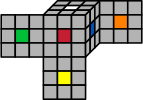
\includegraphics[width=\linewidth]{./images/moving_cubies.png}
\end{image}%
\end{investigation}%
\begin{investigation}{}{x:investigation:invest-edge-cubies}%
In this investigation we'll consider the edge cubies. Hold your Cube with the white center cubie facing up and the red center cubie facing you.%
\begin{enumerate}
\item{}How many edge cubies are there?%
\item{}How many stickers does an edge cubie have?%
\item{}Can you move an edge cubie to a position other than an edge? Explain your reasoning.%
\item{}Identify all the positions on the Cube to which an edge cubie can be moved while keeping the white center cubie on top and red in front.%
\end{enumerate}
As always, make sure you can explain your answers.%
\begin{image}{0.25}{0.5}{0.25}%
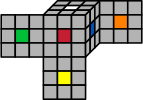
\includegraphics[width=\linewidth]{./images/moving_cubies.png}
\end{image}%
\end{investigation}%
\begin{investigation}{}{x:investigation:invest-center-cubies}%
In this investigation we'll consider the center cubies. Hold your Cube with the white center cubie facing up and the red center cubie facing you.%
\begin{enumerate}
\item{}How many center cubies are there?%
\item{}How many stickers does an center cubie have?%
\item{}Can you move a center cubie to a position other than a center? Explain your reasoning.%
\item{}Identify all the positions on the Cube to which a center cubie can be moved while keeping the white center cubie on top and red in front.%
\end{enumerate}
As always, make sure you can explain your answers.%
\begin{image}{0.25}{0.5}{0.25}%
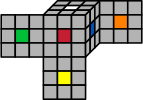
\includegraphics[width=\linewidth]{./images/moving_cubies.png}
\end{image}%
\end{investigation}%
\begin{assemblage}{Question.}{g:assemblage:idp105544717921168}%
How can you tell when a cubie is in the correct \emph{location}? How can you tell when it is \emph{oriented} correctly? Is there a difference?\footnotemark{}%
\end{assemblage}
\footnotetext[1]{Does it depend on the cubie?\label{g:fn:idp105544717922832}}%
\end{subsectionptx}
\end{sectionptx}
%
%
\typeout{************************************************}
\typeout{Section 1.2 Exploring and Describing the Cube}
\typeout{************************************************}
%
\begin{sectionptx}{Exploring and Describing the Cube}{}{Exploring and Describing the Cube}{}{}{x:section:sec-play-exploring-the-cube}
\begin{assemblage}{Motivating Questions.}{g:assemblage:idp105544717924368}%
In this section, we will explore the following questions. %
\begin{enumerate}
\item{}What are faces and layers, and what methods exist for solving them?%
\item{}How can we describe a complex series of Cube moves?%
\item{}What is the order of a Cube move?%
\end{enumerate}
%
\end{assemblage}
\begin{introduction}{}%
In this section, we'll define a few terms and work on an initial exploration of the Cube's white layer. Then, we'll discuss the need for a precise method communicating about our Cubes, and introduce some standard notation.%
\end{introduction}%
%
%
\typeout{************************************************}
\typeout{Subsection 1.2.1 Faces and Layers}
\typeout{************************************************}
%
\begin{subsectionptx}{Faces and Layers}{}{Faces and Layers}{}{}{g:subsection:idp105544717926672}
We begin with a definition.%
\begin{definition}{}{x:definition:def-cube-face}%
\index{Cube facesolved}%
A \terminology{face} of the Cube refers to one of its sides. We say a face is \terminology{solved} if all the stickers on that side are the same color.%
\end{definition}
There are many ways to solve the Cube, and we'll explore one approach later in this chapter. A crucial step in learning to solve the Cube is learning to solve one face.%
\begin{assemblage}{Challenge.}{g:assemblage:idp105544717930000}%
Scramble your Cube. Then solve the white face. If you have not done this before (or even if you have), this may take hours or days, not minutes! Avoid relying on any outside resources (including websites, friends, etc.). When you solve it, congratulations! Then scramble the face and solve it again. Repeat this process until you can reliably do it in just a few minutes. Once you can reliably solve the white face, describe, in writing, your methods as clearly and precisely as you can. What challenges did you have to overcome? How did you overcome them?%
\end{assemblage}
Congratulations on solving a face of your Cube! But a question comes to mind. When your white face is in its solved state, are all the cubies on the white face in the correct location?%
\begin{definition}{}{x:definition:def-cube-layer}%
\index{Cube layersolved}%
A \terminology{layer} of the Cube consists of a face and all of the stickers on Cubies which compose the face. A layer is \terminology{solved} if all of the Cubies in the layer are in the correct location with the correct orientation.%
\end{definition}
\begin{assemblage}{Challenge.}{g:assemblage:idp105544717704848}%
Scramble your Cube and then solve the white layer. As before, this may take hours or days. When you solve it, congratulations! Scramble it and do it again. Once you can reliably solve the white layer, describe, in writing, your methods as clearly and precisely as you can.%
\end{assemblage}
\end{subsectionptx}
%
%
\typeout{************************************************}
\typeout{Subsection 1.2.2 The Need for Notation}
\typeout{************************************************}
%
\begin{subsectionptx}{The Need for Notation}{}{The Need for Notation}{}{}{g:subsection:idp105544717705872}
\begin{principle}{}{}{x:principle:discussion-verbal-cubie-moves}%
Find a partner. Take turns describing verbally and without pointing to your Cube your method for moving a corner cubie to its proper position. Similarly, verbally describe your method for moving an edge cubie to its proper position.%
\end{principle}
\begin{principle}{}{}{x:principle:discussion-written-cubie-moves}%
As you probably noticed, it is challenging to orally describe complex\slash{}technical ideas in much detail without becoming lost. Is it easier to describe your cubie movements in writing? Why or why not?%
\end{principle}
Every area of inquiry has an associated collection of terminology and shorthand notation. At its best, this terminology enables efficient and clear communication. However, terminology can often be a barrier. Thus, we want to avoid introducing unnecessary or confusing jargon whenever possible. However, as I hope \hyperref[x:principle:discussion-verbal-cubie-moves]{Discussion~{\xreffont\ref{x:principle:discussion-verbal-cubie-moves}}} and \hyperref[x:principle:discussion-written-cubie-moves]{Discussion~{\xreffont\ref{x:principle:discussion-written-cubie-moves}}} underscore, a lack of terminology or shorthand notation severely impairs our ability to communicate deep technical ideas. It is with this background that we introduce the following notation, which has become standard in the Cubing community.\begin{aside}{}{g:aside:idp105544717709328}%
\end{aside}
%
\begin{definition}{}{x:definition:def-face-names}%
Hold the Cube in such a way that you are looking at one of the faces.%
\begin{itemize}[label=\textbullet]
\item{}The face you are looking at is referred to as the \terminology{front} (F) face.%
\item{}The face on the side opposite the front is referred to as the \terminology{back} (B) face.%
\item{}The face on the right side is referred to as the \terminology{right} (R) face.%
\item{}The face opposite the right is the \terminology{left} (L) face.%
\item{}The face on the top of the Cube is the \terminology{up} (U) face.%
\item{}The face on the bottom of the Cube is the \terminology{down} (D) face.%
\end{itemize}
A graphical version appears in \hyperref[x:figure:fig-cube-faces]{Figure~{\xreffont\ref{x:figure:fig-cube-faces}}}.%
\begin{figureptx}{}{x:figure:fig-cube-faces}{}%
\begin{image}{0.25}{0.5}{0.25}%
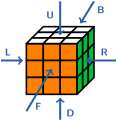
\includegraphics[width=\linewidth]{./images/faces.png}
\end{image}%
\tcblower
\end{figureptx}%
\end{definition}
\begin{activity}{}{g:activity:idp105544717715856}%
List the colors of each of the six faces in \hyperref[x:figure:fig-cube-faces]{Figure~{\xreffont\ref{x:figure:fig-cube-faces}}}.%
\end{activity}%
As we we will see momentarily, the names described in \hyperref[x:definition:def-face-names]{Definition~{\xreffont\ref{x:definition:def-face-names}}} not only help us refer to faces, but also moves of the Cube which help us solve it. In order to understand what a given move does to the Cube, we will need to refer to certain cubies by location. The following definition enables this.%
\begin{definition}{}{x:definition:def-cubie-names}%
A cubie is named by the face(s) on which it sits, using lowercase letters.%
\end{definition}
\begin{activity}{}{x:activity:act-cubie-names}%
Consider the scrambled Cube in \hyperref[x:figure:fig-cubie-names]{Figure~{\xreffont\ref{x:figure:fig-cubie-names}}}.%
%
\begin{enumerate}
\item{}What colors are the \(\ell f u\) cubie?%
\item{}Give the colors of the \(br\) cubie.%
\item{}How can you tell whether the cubie in the named location is a corner or edge cubie?%
\item{}How many letters are required to name a center cubie?%
\item{}Where is the edge cubie that is blue and orange?%
\end{enumerate}
\begin{figureptx}{A scrambled cube.}{x:figure:fig-cubie-names}{}%
\begin{image}{0.25}{0.5}{0.25}%
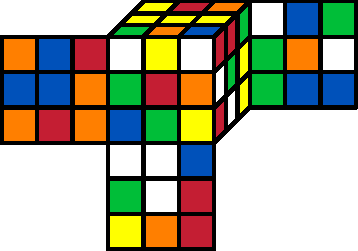
\includegraphics[width=\linewidth]{./images/cubie_names.png}
\end{image}%
\tcblower
\end{figureptx}%
\end{activity}%
We are most interested in using our new notation to describe \emph{moves} of the various faces. We thus make the following definition.%
\begin{definition}{}{x:definition:def-face-moves}%
\index{Cube moveface rotation}%
A given face name, e.g., \(R\), describes a \(90^\circ\) clockwise turn of that face, \emph{as you look at the face}. A given face name with prime symbol, e.g., \(R'\), denotes a \(90^\circ\) counterclockwise turn of that face, \emph{as you look at the face}. A sequence of face moves is written multiplicatively, left to right. We may use parentheses and exponents to write our moves more compactly.%
\end{definition}
\begin{exploration}{}{x:exploration:expl-turning-faces}%
Consider the following questions in the context of a completely solved cube as pictured in \hyperref[x:figure:fig-solved-cube]{Figure~{\xreffont\ref{x:figure:fig-solved-cube}}}.%
%
\begin{enumerate}
\item{}After performing the move \(R\), what color(s) will be on the Up face?%
\item{}Again starting from a solved cube, perform the move \(L\). What color(s) are on the Up face?%
\item{}Explain the difference in your answers to the first two questions.%
\item{}How are \(F^3\) and \(F'\) related?%
\item{}Consider the Cube move \(RF^2 U (LDR)^3\). Which face will you turn first: the left face, or the front face?%
\item{}Again consider the Cube move \(RF^2 U (LDR)^3\). How many times in this move will we turn the right face?%
\item{}What would it mean for two cube moves to be \terminology{equal}? Test your definition by determining whether \(LD = DL\).%
\item{}Suppose \(X\) and \(Y\) are two cube moves. When, if ever, is \(XY = YX\)?%
\end{enumerate}
\begin{figureptx}{A solved cube.}{x:figure:fig-solved-cube}{}%
\begin{image}{0.25}{0.5}{0.25}%
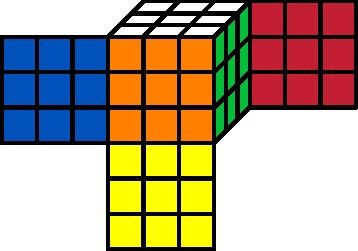
\includegraphics[width=\linewidth]{./images/solved_cube_sf.png}
\end{image}%
\tcblower
\end{figureptx}%
\end{exploration}%
\end{subsectionptx}
%
%
\typeout{************************************************}
\typeout{Subsection 1.2.3 Order}
\typeout{************************************************}
%
\begin{subsectionptx}{Order}{}{Order}{}{}{g:subsection:idp105544717735696}
A useful algebraic concept for describing Cube moves is that of \emph{order}.%
\begin{definition}{}{x:definition:def-order}%
\index{Cube moveorder}%
The \terminology{order} of a cube move \(M\) is the least number of times \(n \gt 1\) that \(M\) can be repeated before a solved Cube is solved again. We write \(|M| = n\).%
\end{definition}
\begin{example}{}{g:example:idp105544717740304}%
The order of \(R\) is 4, since 4 clockwise quarter-turns of the right face of a solved Cube results in a solved Cube, and no fewer number of turns results in a solved Cube.%
\end{example}
\begin{exploration}{}{g:exploration:idp105544717741200}%
%
\begin{enumerate}
\item{}What is \(|U^2|\)?%
\item{}Calculate \(|R^3|\). Why does this make sense?%
\item{}Calculate \(|RUR' U '|\).%
\end{enumerate}
\end{exploration}%
\end{subsectionptx}
\begin{conclusion}{Conclusion.}%
In this section, we began a systematic exploration of the properties of the Cube. First, we described the need for a notational shorthand in solving the white face and layer.%
\par
The standard notation refers to each face \emph{as you look at it}, ignoring color, and describes a \(90^\circ\) clockwise turn of the face. So, \(FR\) means to first turn the front face \(90^\circ\) clockwise, then the right face \(90^\circ\) clockwise. We then noted that we can refer to a cubie by describing the face(s) on which it sits (using lowercase letters to distinguish cubies from faces): three letters refer to a corner, as it sits at the intersection of three faces; two letters refer to an edge, and one to a center.%
\par
We concluded by introducing the idea of order, which will help us analyze and understand more complex sequences of Cube moves in the next section.%
\end{conclusion}%
\end{sectionptx}
%
%
\typeout{************************************************}
\typeout{Section 1.3 Moving Cubies}
\typeout{************************************************}
%
\begin{sectionptx}{Moving Cubies}{}{Moving Cubies}{}{}{x:section:sec-play-moving-cubies}
\begin{assemblage}{Motivating Questions.}{g:assemblage:idp105544717747728}%
In this section, we will explore the following questions. %
\begin{enumerate}
\item{}How can we move the corner cubies so they are in the correct location?%
\item{}How can we describe the movement of the middle ``slice'' of our Cube?%
\item{}How can we move the edge cubies so they are in the correct location?%
\end{enumerate}
%
\end{assemblage}
\begin{introduction}{}%
Our goal in this chapter is to explore, and eventually solve, the Cube. To do this, every cubie must be in the correct \emph{location} with the correct \emph{orientation}. In this section, we focus on two moves which will allow us to put the cubies in the correct location. Once they are in the correct location, we'll see moves in the next section which will help us orient them correctly, enabling us to (finally) solve the Cube.%
\end{introduction}%
We begin by considering \hyperref[x:heuristic:cube-move-cr]{Cube Move~{\xreffont\ref{x:heuristic:cube-move-cr}}}.%
\begin{heuristic}{Moving Corners.}{}{x:heuristic:cube-move-cr}%
Consider the following sequence of Cube moves.%
%
\begin{equation*}
U' R' D' R U R' D R
\end{equation*}
\end{heuristic}
\begin{exploration}{}{x:exploration:expl-cube-move-cr}%
The Cube move described in \hyperref[x:heuristic:cube-move-cr]{Cube Move~{\xreffont\ref{x:heuristic:cube-move-cr}}} moves some of the corners on the front face of the Cube.%
%
\begin{enumerate}
\item{}By performing this move several times, identify on the blank Cube below what is happening to the front face of the Cube.%
\item{}Using the cubie notation described in \hyperref[x:definition:def-cubie-names]{Definition~{\xreffont\ref{x:definition:def-cubie-names}}}, describe what happens to the front face of the Cube after performing this move.%
\item{}Given what happens to the front face, exercise your human creativity and suggest a short name\slash{}abbreviation for this move.%
\item{}What is the order of the move?%
\item{}Practice the move until you can reliably execute it.%
\end{enumerate}
\begin{figureptx}{A blank cube.}{x:figure:fig-cube-move-cr}{}%
\begin{image}{0.25}{0.5}{0.25}%
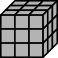
\includegraphics[width=\linewidth]{./images/grey_cube.png}
\end{image}%
\tcblower
\end{figureptx}%
\end{exploration}%
\begin{activity}{}{x:activity:act-cube-move-cr}%
Now that you have identified exactly what \hyperref[x:heuristic:cube-move-cr]{Cube Move~{\xreffont\ref{x:heuristic:cube-move-cr}}} does, use it to solve as much of your Cube it enables.%
\end{activity}%
In order to move the edges, it will be helpful to add one more type of fundamental Cube move to our repertoire.%
\begin{definition}{}{x:definition:def-sr}%
\index{Cube movemiddle slice}%
By \(S_R\) we mean a clockwise rotation of the (vertical) middle slice \emph{as we look at the right face}.%
\begin{sidebyside}{3}{0.0416666666666667}{0.0416666666666667}{0.0833333333333333}%
\begin{sbspanel}{0.3}[center]%
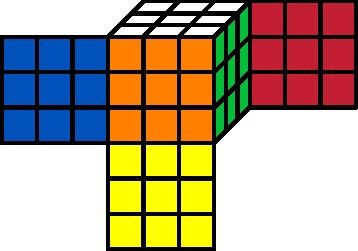
\includegraphics[width=\linewidth]{./images/solved_cube.png}
\end{sbspanel}%
\begin{sbspanel}{0.15}[center]%
%
\begin{equation*}
\underrightarrow{\quad S_R\quad}
\end{equation*}
%
\end{sbspanel}%
\begin{sbspanel}{0.3}[center]%

\includegraphics[width=\linewidth]{./images/middle_slice.png}
\end{sbspanel}%
\end{sidebyside}%
\end{definition}
\begin{heuristic}{Moving Edges.}{}{x:heuristic:cube-move-er}%
\index{Cube movemoving edges}%
Consider the following sequence of Cube moves.%
%
\begin{equation*}
S_R^2 U' S_R' U^2 S_R U' S_R^2
\end{equation*}
\end{heuristic}
\begin{exploration}{}{x:exploration:expl-cube-move-er}%
The Cube move described in \hyperref[x:heuristic:cube-move-er]{Cube Move~{\xreffont\ref{x:heuristic:cube-move-er}}} moves some of the edges on the up face of the Cube.%
%
\begin{enumerate}
\item{}By performing this move several times, identify on the blank Cube below what is happening to the up face of the Cube.%
\item{}Using the cubie notation described in \hyperref[x:definition:def-cubie-names]{Definition~{\xreffont\ref{x:definition:def-cubie-names}}}, describe what is happens to the up face of the Cube after performing this move.%
\item{}Given what happens to the up face, exercise your human creativity and suggest a short name\slash{}abbreviation for this move.%
\item{}What is the order of the move?%
\item{}Practice the move until you can reliably execute it.%
\end{enumerate}
\begin{figureptx}{A blank cube.}{x:figure:fig-cube-move-e}{}%
\begin{image}{0.25}{0.5}{0.25}%
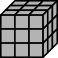
\includegraphics[width=\linewidth]{./images/grey_cube.png}
\end{image}%
\tcblower
\end{figureptx}%
\end{exploration}%
\begin{activity}{}{x:activity:act-cube-move-er}%
Now that you have identified exactly what \hyperref[x:heuristic:cube-move-cr]{Cube Move~{\xreffont\ref{x:heuristic:cube-move-cr}}} and \hyperref[x:heuristic:cube-move-er]{Cube Move~{\xreffont\ref{x:heuristic:cube-move-er}}} do, use them to put every cubie on your Cube in its correct location.%
\end{activity}%
\begin{conclusion}{Conclusion.}%
In this section, we focused on two moves that enable us to put our cubies in the correct location. We first found \hyperref[x:heuristic:cube-move-cr]{Cube Move~{\xreffont\ref{x:heuristic:cube-move-cr}}}, which affects corners on the front face, and no other cubies. Similarly, \hyperref[x:heuristic:cube-move-er]{Cube Move~{\xreffont\ref{x:heuristic:cube-move-er}}} affects edges on the up face, and no other cubies. We were then able to put every cubie on our Cube in the correct location. Hurray!%
\end{conclusion}%
%
%
\typeout{************************************************}
\typeout{Exercises 1.3 Exercises}
\typeout{************************************************}
%
\begin{exercises-subsection-numberless}{Exercises}{}{Exercises}{}{}{g:exercises:idp105544717772560}
\begin{divisionexercise}{1}{}{}{x:exercise:exer-scrambled-edges}%
Consider the state of Lila's Cube in \hyperref[x:figure:fig-scrambled-edges]{Figure~{\xreffont\ref{x:figure:fig-scrambled-edges}}}. She is so close to solving it! Can you help her finish?%
\begin{figureptx}{}{x:figure:fig-scrambled-edges}{}%
\begin{image}{0.25}{0.5}{0.25}%
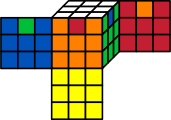
\includegraphics[width=\linewidth]{./images/scrambled_edges.png}
\end{image}%
\tcblower
\end{figureptx}%
\end{divisionexercise}%
\begin{divisionexercise}{2}{}{}{g:exercise:idp105544717774864}%
Sam is nearly done with his Cube; it's pictured in \hyperref[x:figure:fig-edges-corners]{Figure~{\xreffont\ref{x:figure:fig-edges-corners}}}. Can you help him finish?%
\begin{figureptx}{}{x:figure:fig-edges-corners}{}%
\begin{image}{0.25}{0.5}{0.25}%
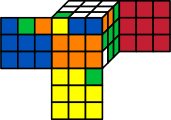
\includegraphics[width=\linewidth]{./images/edges-corners.png}
\end{image}%
\tcblower
\end{figureptx}%
\end{divisionexercise}%
\begin{divisionexercise}{3}{}{}{g:exercise:idp105544717776528}%
Thanks to your help, Lila solved her Cube in \hyperlink{x:exercise:exer-scrambled-edges}{Exercise~{\xreffont 1.3.1}}, but now she needs more help! Can you help her finish the Cube pictured in \hyperref[x:figure:fig-edge-on-bottom]{Figure~{\xreffont\ref{x:figure:fig-edge-on-bottom}}}?%
\begin{figureptx}{}{x:figure:fig-edge-on-bottom}{}%
\begin{image}{0.25}{0.5}{0.25}%
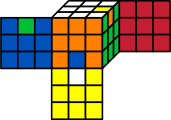
\includegraphics[width=\linewidth]{./images/edge_on_bottom.png}
\end{image}%
\tcblower
\end{figureptx}%
\end{divisionexercise}%
\begin{divisionexercise}{4}{}{}{g:exercise:idp105544717778576}%
Consider the situation in \hyperref[x:figure:fig-scrambled-corners]{Figure~{\xreffont\ref{x:figure:fig-scrambled-corners}}}. Why will \hyperref[x:heuristic:cube-move-cr]{Cube Move~{\xreffont\ref{x:heuristic:cube-move-cr}}} alone be insufficient for putting the corners in their correct locations? Devise a strategy for putting the corners in the correct locations.%
\begin{figureptx}{}{x:figure:fig-scrambled-corners}{}%
\begin{image}{0.25}{0.5}{0.25}%
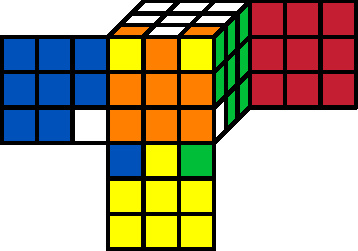
\includegraphics[width=\linewidth]{./images/scrambled_corners.png}
\end{image}%
\tcblower
\end{figureptx}%
\end{divisionexercise}%
\end{exercises-subsection-numberless}
\end{sectionptx}
%
%
\typeout{************************************************}
\typeout{Section 1.4 Reorienting Cubies}
\typeout{************************************************}
%
\begin{sectionptx}{Reorienting Cubies}{}{Reorienting Cubies}{}{}{x:section:sec-play-reorienting-cubies}
\begin{assemblage}{Motivating Questions.}{g:assemblage:idp105544717781520}%
In this section, we will explore the following questions. %
\begin{enumerate}
\item{}How can we change the orientation of the corner cubies?%
\item{}How can we change the orientation of the edge cubies?%
\item{}How can we apply our four Cube moves to solve the Cube?%
\end{enumerate}
%
\end{assemblage}
\begin{introduction}{}%
In \hyperref[x:section:sec-play-moving-cubies]{Section~{\xreffont\ref{x:section:sec-play-moving-cubies}}}, we considered ways of moving certain edge and corner cubies. The key that allows us to use \hyperref[x:heuristic:cube-move-cr]{Cube Move~{\xreffont\ref{x:heuristic:cube-move-cr}}} and \hyperref[x:heuristic:cube-move-er]{Cube Move~{\xreffont\ref{x:heuristic:cube-move-er}}} to put your cubies in the correct location is that each move affects precisely three cubies. All others are left unmoved. By using just \hyperref[x:heuristic:cube-move-cr]{Cube Move~{\xreffont\ref{x:heuristic:cube-move-cr}}} and \hyperref[x:heuristic:cube-move-er]{Cube Move~{\xreffont\ref{x:heuristic:cube-move-er}}}, we can thus put each cubie in the correct location. However, even if a cubie is in the correct location, it may be that its stickers are on the wrong faces\textemdash{}in this case, it needs to be \emph{reoriented}.%
\par
In this section, we will see how to reorient cubies once they are in the correct location. To do so, we'll learn two moves: one that reorients corners, and one that reorients edges. Once we are able to put each cubie in the correct location, and then orient it correctly, each scrambled Cube becomes a puzzle, solvable by clever application of these moves.%
\end{introduction}%
We begin by exploring a move that reorients two corners.%
\begin{heuristic}{}{}{x:heuristic:cube-move-co}%
\index{Cube movereorienting corners}%
Consider the following sequence of Cube moves.%
%
\begin{equation*}
(R' D^2 R B' U^2 B)^2
\end{equation*}
\end{heuristic}
\begin{exploration}{Reorienting Corners.}{x:exploration:expl-cube-move-co}%
The Cube move described in \hyperref[x:heuristic:cube-move-co]{Cube Move~{\xreffont\ref{x:heuristic:cube-move-co}}} reorients two corners: one on the Up face, and one on the Down face.%
%
\begin{enumerate}
\item{}By performing this move several times, identify on the blank Cube below what is happening to the Up face of the Cube. Describe what is happening to the Down face as well.%
\item{}Using the cubie notation described in \hyperref[x:definition:def-cubie-names]{Definition~{\xreffont\ref{x:definition:def-cubie-names}}}, describe what is happens to the Up and Down faces of the Cube after performing this move.%
\item{}Given what this move does, exercise your human creativity and suggest a short name\slash{}abbreviation for this move.%
\item{}What is the order of the move?%
\item{}Practice the move until you can reliably execute it.%
\end{enumerate}
\begin{figureptx}{A blank cube.}{x:figure:fig-cube-move-e}{}%
\begin{image}{0.25}{0.5}{0.25}%
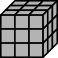
\includegraphics[width=\linewidth]{./images/grey_cube.png}
\end{image}%
\tcblower
\end{figureptx}%
\end{exploration}%
Our last Cube move will reorient two edge cubies. Recall \hyperref[x:definition:def-sr]{Definition~{\xreffont\ref{x:definition:def-sr}}}.%
\begin{heuristic}{}{}{x:heuristic:cube-move-eo}%
\index{Cube movereorienting edges}%
Consider the following sequence of Cube moves.%
%
\begin{equation*}
(S_R U)^3 U (S_R ' U)^3 U
\end{equation*}
\end{heuristic}
\begin{exploration}{Reorienting Edges.}{x:exploration:expl-cube-move-co}%
The Cube move described in \hyperref[x:heuristic:cube-move-co]{Cube Move~{\xreffont\ref{x:heuristic:cube-move-co}}} reorients two edges on the Up face.%
%
\begin{enumerate}
\item{}By performing this move several times, identify on the blank Cube below what is happening to the Up face of the Cube.%
\item{}Using the cubie notation described in \hyperref[x:definition:def-cubie-names]{Definition~{\xreffont\ref{x:definition:def-cubie-names}}}, describe what is happens to the Up face of the Cube after performing this move.%
\item{}Given what this move does, exercise your human creativity and suggest a short name\slash{}abbreviation for this move.%
\item{}What is the order of the move?%
\item{}Practice the move until you can reliably execute it.%
\end{enumerate}
\begin{figureptx}{A blank cube.}{x:figure:fig-cube-move-e}{}%
\begin{image}{0.25}{0.5}{0.25}%
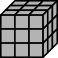
\includegraphics[width=\linewidth]{./images/grey_cube.png}
\end{image}%
\tcblower
\end{figureptx}%
\end{exploration}%
\begin{assemblage}{Solving the Cube.}{g:assemblage:idp105544717766672}%
When you can consistently perform \hyperref[x:heuristic:cube-move-cr]{Cube Move~{\xreffont\ref{x:heuristic:cube-move-cr}}}, \hyperref[x:heuristic:cube-move-co]{Cube Move~{\xreffont\ref{x:heuristic:cube-move-co}}}, \hyperref[x:heuristic:cube-move-er]{Cube Move~{\xreffont\ref{x:heuristic:cube-move-er}}}, and \hyperref[x:heuristic:cube-move-eo]{Cube Move~{\xreffont\ref{x:heuristic:cube-move-eo}}}, you can use them to solve the Cube. You can use any strategy you want, but here is one to consider.%
\begin{enumerate}
\item{}Put the corners in the correct \emph{location}.%
\item{}Put the edges in the correct \emph{location}.%
\item{}\emph{Reorient} any corners that need reorienting.%
\item{}\emph{Reorient} any edges that need reorienting.%
\item{}\emph{Celebrate!}%
\item{}Scramble the Cube and do it again.%
\end{enumerate}
%
\end{assemblage}
\begin{conclusion}{Conclusion.}%
In this section, we explored the last moves we need to solve the Cube. We also described a strategy for solving the Cube. Our method of solving the Cube is based on the \emph{corners-first} (CF) method, which is distinct from the layer-by-layer (LL) method which is often the first solving method people learn. The first solution to the Cube, by Erno Rubik himself, was corners-first, and the first world speed-cubing record (22.95 seconds) was done corners-first.%
\par
There are advantages and disadvantages to all solution methods. Advantages to corners-first are:%
\begin{itemize}[label=\textbullet]
\item{}The move sequences are generally shorter in CF%
\item{}There are just a few important move sequences to memorize%
\item{}You generally don't "break" your existing work and so can recover from mistakes more easily%
\item{}The solution can scale from a leisurely solve of a few minutes or more to quite fast solves%
\end{itemize}
%
\end{conclusion}%
%
%
\typeout{************************************************}
\typeout{Exercises 1.4 Exercises}
\typeout{************************************************}
%
\begin{exercises-subsection-numberless}{Exercises}{}{Exercises}{}{}{g:exercises:idp105544717807632}
\begin{divisionexercise}{1}{}{}{g:exercise:idp105544717808144}%
Sam is nearly done with his Cube! Which of the Cube moves from this section does he need? How many times will he have to perform it?%
\begin{figureptx}{}{x:figure:fig-exercise-co}{}%
\begin{image}{0.25}{0.5}{0.25}%
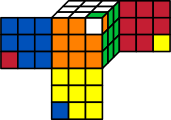
\includegraphics[width=\linewidth]{./images/co.png}
\end{image}%
\tcblower
\end{figureptx}%
\end{divisionexercise}%
\begin{divisionexercise}{2}{}{}{g:exercise:idp105544717809424}%
Lila is nearly done with her Cube! Which move from this section will be helpful? How should she use it?%
\begin{figureptx}{}{x:figure:fig-exercise-eo}{}%
\begin{image}{0.25}{0.5}{0.25}%
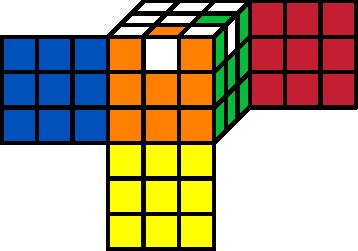
\includegraphics[width=\linewidth]{./images/eo-exer.png}
\end{image}%
\tcblower
\end{figureptx}%
\end{divisionexercise}%
\begin{divisionexercise}{3}{}{}{g:exercise:idp105544717810832}%
Sam has gotten himself into a bit of a pickle. How can he apply our moves to solve his Cube?%
\begin{figureptx}{}{x:figure:fig-exercise-co-move}{}%
\begin{image}{0.25}{0.5}{0.25}%
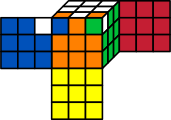
\includegraphics[width=\linewidth]{./images/co02.png}
\end{image}%
\tcblower
\end{figureptx}%
\end{divisionexercise}%
\begin{divisionexercise}{4}{}{}{g:exercise:idp105544717812112}%
This configuration is known as the \terminology{superflip}. Describe what you see. Can you achieve this on your Cube?%
\begin{figureptx}{}{x:figure:fig-exer-superflip}{}%
\begin{image}{0.25}{0.5}{0.25}%
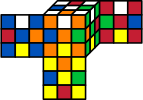
\includegraphics[width=\linewidth]{./images/superflip.png}
\end{image}%
\tcblower
\end{figureptx}%
\end{divisionexercise}%
\end{exercises-subsection-numberless}
\end{sectionptx}
\end{chapterptx}
\end{partptx}
%
%
\typeout{************************************************}
\typeout{Part II Truth}
\typeout{************************************************}
%
\begin{partptx}{Truth}{}{Truth}{}{}{x:part:part-truth}
 As Su identifies in \hyperlink{x:biblio:Su2020}{[{\xreffont 1}]}, humans have an innate desire for truth. Defining just what we mean by \terminology{truth} is tricky, so we'll follow Su's lead and just say that ``true statements are ones that align with reality''. In an age of rampant disinformation, we seek to know what is actually true.%
\par
Mathematics is often thought of as one of the last bastions of objective truth. One widely accepted cultural norm is that if a statement is quantitative, or can be arrived at via a sequence of logical deductions, it is often considered "true", whereas statements that cannot be presented in such a way live in the realm of opinion. Yet, mathematics is a human endeavor; and what do mathematicians mean when they talk of a statement being ``true'', anyway? The answer might surprise you.%
\par
In this unit, we'll explore inductive and deductive reasoning, as well as formal logic. We'll explore the shortcomings of mathematical thinking in addition to its strengths.%
\par
This chapter is heavily influenced by \emph{\href{https://www.artofmathematics.org/books/truth-reasoning-certainty-and-proof}{Discovering the Art of Mathematics: Truth, Reasoning, Certainty, and Proof}\footnote{\nolinkurl{https://www.artofmathematics.org/books/truth-reasoning-certainty-and-proof}\label{g:fn:idp105544717785488}}} by Fleron, Hotchkiss, Ecke, and von Renesse.%
 %
%
\typeout{************************************************}
\typeout{Chapter 2 Inductive and Deductive Reasoning}
\typeout{************************************************}
%
\begin{chapterptx}{Inductive and Deductive Reasoning}{}{Inductive and Deductive Reasoning}{}{}{x:chapter:chap-reasoning}
\begin{introduction}{}%
In order to  more fully explore the deductive reasoning employed in mathematical explorations, we'll first contrast it with the inductive reasoning common in other areas of inquiry.%
\par
WRITE MORE HERE%
\end{introduction}%
%
%
\typeout{************************************************}
\typeout{Section 2.1 Inductive Reasoning}
\typeout{************************************************}
%
\begin{sectionptx}{Inductive Reasoning}{}{Inductive Reasoning}{}{}{g:section:idp105544717787536}
\begin{assemblage}{Motivating Questions.}{g:assemblage:idp105544717788304}%
In this section, we will explore the following questions. %
\begin{enumerate}
\item{}What is truth? What is fact? Is there a difference?%
\item{}What is inductive reasoning? When is it helpful? What are its shortcomings?%
\end{enumerate}
%
\end{assemblage}
We'll begin by attempting to define \emph{truth} and \emph{fact}, and compare them. We'll then explore \emph{inductive reasoning} in depth, considering its benefits shortcomings.%
\begin{principle}{}{}{g:principle:idp105544717791376}%
What is truth? What is fact? How are the two concepts related? How are they different? Under which category does the sentence \(1+1=2\) fall?%
\end{principle}
\begin{activity}{What's my world?}{x:activity:act-whats-my-world}%
In the game \emph{What's my World?}, one person thinks of a single law that defines a hypothetical world (e.g., ``My world does not contain things that start with the letter 'C'.''). The other players attempt to guess this governing law by taking turns asking questions of the creator, such as ``Does your world contain dogs? Does it contain cats?'' and so on. When one of the guessers believe they can identify the governing law, they ask the creator.%
\par
Play a few rounds of this game, taking turns in the role of creator. \emph{Other than asking the creator directly}, how could you be \emph{certain} that you had determined the law of the world?%
\end{activity}%
\begin{definition}{}{g:definition:idp105544717796624}%
\index{inductive reasoning}%
\terminology{Inductive reasoning} is the process of drawing general conclusions from particular instances, generally known as \terminology{data}.%
\end{definition}
The work of the guesser in \hyperref[x:activity:act-whats-my-world]{Activity~{\xreffont\ref{x:activity:act-whats-my-world}}} is to employ inductive reasoning to determine the general law put in place by the creator. This is the scientific process at its best: looking at the world in its orderliness and using our curiosity and creativity to infer larger governing principles. If you have taken a statistics course, this is the type of reasoning employed there.%
\par
But how does this work in mathematics?%
\begin{exploration}{}{x:exploration:expl-dot-game}%
Let's play a game with dots and lines. We'll start with at least two dots (though you'll probably want to increase this number pretty quickly). The rules are:%
%
\begin{itemize}[label=\textbullet]
\item{}Split your dots into two groups, group \(A\) and group \(B\), and draw each group on its own line.%
\item{}Connect (some of) the dots from \(A\) to (some of) the dots in \(B\) with lines. The lines don't have to be straight\textemdash{}they can curve in any way you want!\textemdash{}but each line should connect precisely two dots: one from \(A\) and one from \(B\).%
\item{}Each dot should be connected to at least one other dot\textemdash{}no lonely dots!%
\end{itemize}
So, if I label four dots as \(X, Y, Z, W\), \emph{one possible} drawing is given in \hyperref[x:figure:fig-dot-game-example]{Figure~{\xreffont\ref{x:figure:fig-dot-game-example}}}.%
\begin{figureptx}{}{x:figure:fig-dot-game-example}{}%
\begin{image}{0.325}{0.35}{0.325}%
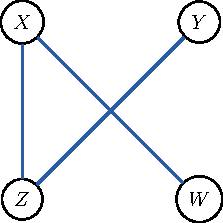
\includegraphics[width=\linewidth]{./images/dot-game-example.png}
\end{image}%
\tcblower
\end{figureptx}%
However, there is a problem with this drawing: the lines cross! I know, this wasn't one of the rules above, but let's add it.%
%
\begin{itemize}[label=\textbullet]
\item{}The lines can be drawn so that none of them cross.%
\end{itemize}
Now consider the following questions.%
%
\begin{enumerate}
\item{}Redraw the picture in \hyperref[x:figure:fig-dot-game-example]{Figure~{\xreffont\ref{x:figure:fig-dot-game-example}}} so that none of the lines cross.%
\item{}Give a name to drawings of figures like \hyperref[x:figure:fig-dot-game-example]{Figure~{\xreffont\ref{x:figure:fig-dot-game-example}}} which \emph{can} be drawn so that none of the lines cross.%
\item{}Which drawings are possible with two or three dots? Can they be drawn to have the property that none of the lines cross?%
\item{}What other drawings are possible with four dots? Five?%
\item{}Based on your work here, do you think it will always be possible to draw these pictures so that none of the lines cross? Explain your thinking.%
\end{enumerate}
\end{exploration}%
\begin{principle}{}{}{g:principle:idp105544718104336}%
Based on our work in this section, what are some strengths of inductive reasoning? What are some possible pitfalls? How can we minimize these potential downsides?%
\end{principle}
%
%
\typeout{************************************************}
\typeout{Exercises 2.1 Exercises}
\typeout{************************************************}
%
\begin{exercises-subsection-numberless}{Exercises}{}{Exercises}{}{}{g:exercises:idp105544718104848}
\begin{divisionexercise}{1}{}{}{g:exercise:idp105544718105360}%
Do some internet research on the \terminology{Twin Prime Conjecture}. What is it? When was it first formulated? Is it true? Likely true?%
\end{divisionexercise}%
\end{exercises-subsection-numberless}
\end{sectionptx}
%
%
\typeout{************************************************}
\typeout{Section 2.2 Deductive Reasoning}
\typeout{************************************************}
%
\begin{sectionptx}{Deductive Reasoning}{}{Deductive Reasoning}{}{}{g:section:idp105544718106384}
\begin{assemblage}{Motivating Questions.}{g:assemblage:idp105544718107152}%
In this section, we will explore the following questions. %
\begin{enumerate}
\item{}What is deductive reasoning? How does it differ from inductive reasoning?%
\item{}How is deductive reasoning employed in mathematics?%
\item{}What are some strengths and weaknesses of deductive reasoning?%
\end{enumerate}
%
\end{assemblage}
Formal mathematical reasoning is deductive (defined momentarily), and begins with \terminology{axioms}, which are statements that should be self-evident and taken to be true. Note that while axioms are not always explicitly stated, they \emph{can} be when necessary.%
\begin{investigation}{}{g:investigation:idp105544718110096}%
The most famous set of axioms are Euclid's postulates for geometry, defined in \emph{\href{https://en.wikipedia.org/wiki/Euclid's_Elements}{The Elements}\footnotemark{}}, which not only shaped thousands of years of geometry, but solidified the deductive approach to doing and explaining mathematics that we will explore in this unit. At the beginning of Book I of \emph{The Elements}, Euclid identified five postulates and five axioms.%
\par
Euclid's \emph{postulates} are:%
%
\begin{enumerate}
\item{}A straight line segment can be drawn joining any two points.%
\item{}Any straight line segment can be extended indefinitely in a straight line.%
\item{}Any circle can be described given a center and (radial) distance.%
\item{}All right angles are equal to one another.%
\item{}If a straight line intersecting two straight lines make the interior angles on the same side less than two right angles, the two straight lines, if produced indefinitely, meet on the side on which the angles are less than two right angles.%
\end{enumerate}
Euclid's \emph{axioms} (or \emph{common notions}) are:%
%
\begin{enumerate}
\item{}Things which are equal to the same thing are also equal to one another.%
\item{}If equals are added to equals, the wholes are equal.%
\item{}If equals are subtracted from equals, the remainders are equal.%
\item{}Things which coincide with one another are equal to one another.%
\item{}The whole is greater than the part.%
\end{enumerate}
The desired qualities of a system of axioms are:%
%
\begin{enumerate}
\item{}\terminology{consistency}: we cannot deduce contradictory propositions, such as "God exists" and "God does not exist" from the same set of axioms%
\item{}\terminology{simplicity}: we have as few axioms as possible, and they are no more complicated than they need to be%
\item{}\terminology{completeness}: the system can answer every question we can think to ask%
\end{enumerate}
In your groups, discuss Euclid's postulates and common notions, perhaps in view of the desired qualities of an axiomatic system. What strikes you as being interesting or noteworthy? Make a list of at least 2-3 observations. Then consider: on what axioms or assumptions do you make decisions (e.g., about how to spend your time, resources, etc)?%
\end{investigation}%
\footnotetext[1]{\nolinkurl{https://en.wikipedia.org/wiki/Euclid's_Elements}\label{g:fn:idp105544718111376}}%
The process of \terminology{deductive reasoning} in mathematics begins from a set of generally agreed-upon axioms of \href{https://en.wikipedia.org/wiki/Zermelo–Fraenkel_set_theory}{set theory}\footnote{\nolinkurl{https://en.wikipedia.org/wiki/Zermelo–Fraenkel_set_theory}\label{g:fn:idp105544718088592}}\footnote{It should be noted that there is disagreement about the Axiom of Choice, mostly due to some of its surprising consequences.\label{g:fn:idp105544718088848}} and uses logic to make inevitable conclusions from those axioms. These conclusions are generally called \terminology{theorems}. They are usually given as conditional statements of the form ``If \(P\), then \(Q\),'' where \(P\) and \(Q\) are sensible\begin{aside}{}{g:aside:idp105544718091664}%
\end{aside}
 statements. Moreover, since most deductive statements are presented in conditional form, their scope is generally limited. That is, the statement ``if it is Monday, then we have math class'' is only making a claim about what happens on Mondays; it says nothing whatsoever about any other day of the week. We will explore the consequences of this more in \hyperref[x:chapter:chap-logic]{Chapter~{\xreffont\ref{x:chapter:chap-logic}}}.%
\par
The author Lewis Carroll loved logic puzzles (he was actually a mathematics professor!), and wrote many of them. Here is one, axiomatized for easy reference.%
\begin{axiom}{(Carroll).}{}{x:axiom:axiom-kittens}%
Consider the axioms:%
%
\begin{enumerate}
\item{}If a kitten loves fish, then it is teachable.%
\item{}Every kitten without a tail will play with a gorilla.%
\item{}All kittens with whiskers love fish.%
\item{}If a kitten has green eyes, then it is not teachable.%
\item{}All kittens have whiskers or do not have tails.%
\end{enumerate}
\end{axiom}
Once you have a deductive argument that (generally) begins from your premises and reasons, step-by-step, to your conclusion, you can write out the argument in a short essay known as a \emph{proof}. For our purposes, a proof is just a \emph{convicing argument}. It should be written at a level appropriate to the reader and clearly lay out the steps necessary for a reader who accepts your hypotheses to believe the conclusion. As an example, consider the following.%
\begin{example}{}{x:example:example-kitten-deduction}%
All kittens with whiskers are teachable.%
\par
\terminology{Proof}. Suppose we have a kitten with whiskers. Let's call him Arthur. By \hyperref[x:axiom:axiom-kittens]{Axiom~{\xreffont\ref{x:axiom:axiom-kittens}}} \#3, Arthur loves fish. Since Arthur loves fish, \hyperref[x:axiom:axiom-kittens]{Axiom~{\xreffont\ref{x:axiom:axiom-kittens}}} \#1 implies that Arthur is teachable.%
\par
Since Arthur was an arbitrary kitten, we conclude that all kittens with whiskers are teachable.%
\end{example}
There are several observations which are worth a moment of our time in the proof in \hyperref[x:example:example-kitten-deduction]{Example~{\xreffont\ref{x:example:example-kitten-deduction}}}.%
%
\begin{itemize}[label=\textbullet]
\item{}We first note that the proof is written using standard conventions of academic writing, including complete sentences, proper punctuation and capitalization, etc. This is important! In order to convince someone that your argument is valid, they need to be able to read it.%
\item{}While the statement to be proved is not written as ``if \(P\), then \(Q\)'', it \emph{can} be stated that way: ``If \(A\) is a kitten with whiskers, then \(A\) is teachable''. Thus, our proof begins by considering an arbitrary kitten with whiskers, who we name Arthur. We observe, however, that there is nothing special about Arthur that figures into our proof in a meaningful way, so the argument will apply just as well to any kitten with whiskers we may find.%
\item{}In each step we take throughout the proof, we refer to the specific axiom from \hyperref[x:axiom:axiom-kittens]{Axiom~{\xreffont\ref{x:axiom:axiom-kittens}}} that allow us to take that step. It is valuable to be able to do this, but generally we do not specifically refer to the axioms by number. This is to improve the readability of the proof.%
\item{}Finally, note that our proof concludes with a conclusion: all kittens with whiskers are teachable. This is good practice and sends an unmistakable signal to the reader that you are done.%
\end{itemize}
Now, prove the theorems that follow using \hyperref[x:axiom:axiom-kittens]{Axiom~{\xreffont\ref{x:axiom:axiom-kittens}}}.%
\begin{theorem}{}{}{g:theorem:idp105544718137360}%
If a kitten has green eyes, then it does not love fish.%
\end{theorem}
\begin{theorem}{}{}{g:theorem:idp105544718137872}%
If a kitten has a tail, then it does not have green eyes.%
\end{theorem}
\begin{theorem}{}{}{g:theorem:idp105544718139152}%
Every kitten with green eyes will play with a gorilla.%
\end{theorem}
\begin{activity}{}{g:activity:idp105544718139664}%
Compare and contrast the structures of the proofs of the preceding theorems. Can you clarify the general reasoning patterns you used to prove them?%
\end{activity}%
\begin{principle}{}{}{g:principle:idp105544718140432}%
We have now explored both inductive and deductive reasoning. How are they similar? How are they different? How might you decide which type of reasoning to employ in a given situation? What are their strengths and weaknesses?%
\end{principle}
\begin{conclusion}{Conclusion.}%
In this section, we explored deductive reasoning, which begins from accepted axioms and premises and then reasons, step by logical step, toward a conclusion. This is the primary form of reasoning used in mathematics. We saw that while conclusions reached via deductive reasoning are generally tighter and more certain, there are still some drawbacks.%
\par
The main drawback of deductive reasoning involves scope. We must begin with axioms, so the axioms must be well-chosen and sensible. However, if one disagrees with the choice of a set of axioms, then one must be willing to set aside any results deduced from them (or, at least, deduced from the particular axioms with which one disagrees).%
\par
A second drawback having to do with scope concerns the premises of a conditional statement. In particular, if the premises of a statement are not satisfied, the statement makes no assertion whatsoever (though, as we will see in \hyperref[x:chapter:chap-logic]{Chapter~{\xreffont\ref{x:chapter:chap-logic}}}, there is still a \emph{consistent} way to assign truth values to statements whose premises are not satisfied).%
\end{conclusion}%
%
%
\typeout{************************************************}
\typeout{Exercises 2.2 Exercises}
\typeout{************************************************}
%
\begin{exercises-subsection-numberless}{Exercises}{}{Exercises}{}{}{g:exercises:idp105544718142864}
\begin{divisionexercise}{1}{}{}{g:exercise:idp105544718143376}%
Invent one or two additional theorems that can be deduced from \hyperref[x:axiom:axiom-kittens]{Axiom~{\xreffont\ref{x:axiom:axiom-kittens}}}. Prove them.%
\end{divisionexercise}%
\end{exercises-subsection-numberless}
\end{sectionptx}
\end{chapterptx}
 %
%
\typeout{************************************************}
\typeout{Chapter 3 Modern Mathematical Logic}
\typeout{************************************************}
%
\begin{chapterptx}{Modern Mathematical Logic}{}{Modern Mathematical Logic}{}{}{x:chapter:chap-logic}
\begin{introduction}{}%
In \hyperref[x:chapter:chap-reasoning]{Chapter~{\xreffont\ref{x:chapter:chap-reasoning}}}, we explored two types of reasoning: inductive reasoning, and deductive reasoning. The type of reasoning used most often in mathematics is deductive reasoning. In the late 19th\slash{}early 20th century, logic itself was mathematized by the likes of George Boole and Augustus De Morgan into a \emph{propositional calculus}. This gave mathematicians a means of determining the truth value of a statement purely based on its inherent logical structure.%
\par
It is this method of calculating that we explore in this chapter.%
\end{introduction}%
%
%
\typeout{************************************************}
\typeout{Section 3.1 Logical Connectives and Rules of Inference}
\typeout{************************************************}
%
\begin{sectionptx}{Logical Connectives and Rules of Inference}{}{Logical Connectives and Rules of Inference}{}{}{x:section:sec-connectives}
\begin{assemblage}{Motivating Questions.}{g:assemblage:idp105544718115088}%
In this section, we will explore the following questions. %
\begin{enumerate}
\item{}What is a proposition?%
\item{}What are logical connectives? How can they be used to build new propositions?%
\item{}What does it mean for two propositions to be logically equivalent?%
\end{enumerate}
%
\end{assemblage}
In the late 19th and early 20th centuries, mathematicians began mathematize and formalize logic itself. Today we begin to explore these foundational issues. We'll start with some definitions.%
\begin{definition}{}{g:definition:idp105544718117264}%
\index{proposition}%
\index{propositionelementary}%
\index{logical connectives}%
A \terminology{proposition} is a declarative sentence which is either true or false, but not both. An \terminology{elementary proposition} is a sentence with a subject and a verb, but no connectives (such as \emph{and, or, not, if-then,} or \emph{if-and-only-if}).%
\end{definition}
\begin{activity}{}{x:activity:act-propositions}%
Determine which of the following are propositions (elementary or otherwise). If a given sentence is a proposition, determine its truth value. If it isn't, explain why not.%
%
\begin{enumerate}
\item{}Erik Hoekstra is the president of Dordt University.%
\item{}The square root of a whole number is always a whole number.%
\item{}The Green Bay Packers are the worst football team.%
\item{}Why is this class so much fun?%
\item{}This sentence is false.%
\item{}A group of crows is called a murder.%
\item{}Everyone likes cats.%
\end{enumerate}
\end{activity}%
Now that we have a sense for what a proposition is, we'll take old propositions and make new ones using \emph{logical connectives}. In order to describe how the connectives work, mathematicians define the truth values of the new propositions \emph{formally}\textemdash{}that is, without regard to the content of the propositions themselves\textemdash{}in terms of the possible combinations of truth values from the constituent propositions. This gives us an abstract way of considering the truth values of propositions.%
\begin{definition}{}{g:definition:idp105544718127120}%
\index{negation}%
\index{logical connectivesnegation}%
Suppose \(P\) and \(Q\) are statements (e.g., like those in \hyperref[x:activity:act-propositions]{Activity~{\xreffont\ref{x:activity:act-propositions}}}). The \terminology{negation} of \(P\), denoted \(\neg P\) and read "not \(P\)", has the opposite truth value of \(P\) and is defined by \hyperref[x:table:table-negation]{Table~{\xreffont\ref{x:table:table-negation}}}.%
\begin{tableptx}{\textbf{The negation of \(P\).}}{x:table:table-negation}{}%
\centering%
{\tabularfont%
\begin{tabular}{cc}
\multicolumn{1}{lB}{\(​P\)}&\multicolumn{1}{l}{\(​\neg P\)}\tabularnewline\hrulemedium
\multicolumn{1}{cB}{T}&F\tabularnewline[0pt]
\multicolumn{1}{cB}{F}&T
\end{tabular}
}%
\end{tableptx}%
\end{definition}
\begin{definition}{}{g:definition:idp105544718169360}%
\index{and}%
\index{logical connectivesand}%
The \terminology{conjunction} of \(P\) and \(Q\), denoted \(P \land Q\) and read ``\(P\) and \(Q\)'', is true when both \(P\) and \(Q\) are true, and false otherwise. See \hyperref[x:table:table-and]{Table~{\xreffont\ref{x:table:table-and}}}.%
\begin{tableptx}{\textbf{The conjunction of \(P\) and \(Q\).}}{x:table:table-and}{}%
\centering%
{\tabularfont%
\begin{tabular}{ccc}
\multicolumn{1}{lB}{\(​P\)}&\multicolumn{1}{lB}{\(​Q\)}&\multicolumn{1}{l}{\(P \land Q​\)}\tabularnewline\hrulemedium
\multicolumn{1}{cB}{T}&\multicolumn{1}{cB}{T}&T\tabularnewline[0pt]
\multicolumn{1}{cB}{T}&\multicolumn{1}{cB}{F}&F\tabularnewline[0pt]
\multicolumn{1}{cB}{F}&\multicolumn{1}{cB}{T}&F\tabularnewline[0pt]
\multicolumn{1}{cB}{F}&\multicolumn{1}{cB}{F}&F
\end{tabular}
}%
\end{tableptx}%
\end{definition}
\begin{definition}{}{g:definition:idp105544718150544}%
\index{or}%
\index{logical connectivesor}%
The \terminology{disjunction} of \(P\) and \(Q\), denoted \(P \lor Q\) and read ``\(P\) or \(Q\)'', is true when \(P\) is true, \(Q\) is true, or both are true, and false otherwise. See \hyperref[x:table:table-or]{Table~{\xreffont\ref{x:table:table-or}}}.%
\begin{tableptx}{\textbf{The disjunction of \(P\) and \(Q\).}}{x:table:table-or}{}%
\centering%
{\tabularfont%
\begin{tabular}{ccc}
\multicolumn{1}{lB}{\(​P\)}&\multicolumn{1}{lB}{\(​Q\)}&\multicolumn{1}{l}{\(P \lor Q​\)}\tabularnewline\hrulemedium
\multicolumn{1}{cB}{T}&\multicolumn{1}{cB}{T}&T\tabularnewline[0pt]
\multicolumn{1}{cB}{T}&\multicolumn{1}{cB}{F}&T\tabularnewline[0pt]
\multicolumn{1}{cB}{F}&\multicolumn{1}{cB}{T}&T\tabularnewline[0pt]
\multicolumn{1}{cB}{F}&\multicolumn{1}{cB}{F}&F
\end{tabular}
}%
\end{tableptx}%
\end{definition}
\begin{activity}{}{g:activity:idp105544718197264}%
Meaningfully negate the following propositions (without just saying "It is not the case that...").%
%
\begin{enumerate}
\item{}\(e\) is a negative real number.%
\item{}Iowa is the tenth largest state.%
\item{}17 is a prime number.%
\end{enumerate}
\par\smallskip%
\noindent%
\begin{enumerate}
\item{}\(e\) is a nonnegative real number.%
\item{}Iowa is not the tenth largest state.%
\item{}17 is a composite number.%
\end{enumerate}
\end{activity}%
\begin{exploration}{}{g:exploration:idp105544718200592}%
Determine the truth values of the following propositions.%
%
\begin{enumerate}
\item{}Math 149 meets on Mondays and the capital of Iowa is Des Moines.%
\item{}Math 149 meets on Mondays and the capital of Minnesota is Minneapolis.%
\item{}Math 149 meets on Mondays or the capital of Minnesota is Minneapolis.%
\end{enumerate}
\end{exploration}%
The last connective we'll consider (for now) is \emph{implication}.%
\begin{definition}{}{x:definition:def-implications}%
\index{implication}%
\index{if-then}%
\index{conditional statements}%
\index{logical connectivesimplies}%
Let \(P\) and \(Q\) be statements. The \terminology{implication}, "\(P\) implies \(Q\)" (or "if \(P\), then \(Q\)") is denoted \(P\Rightarrow Q\), and is false only when \(P\) is true but \(Q\) is false. See \hyperref[x:table:table-implication]{Table~{\xreffont\ref{x:table:table-implication}}}.%
\begin{tableptx}{\textbf{The implication \(P\Rightarrow Q\).}}{x:table:table-implication}{}%
\centering%
{\tabularfont%
\begin{tabular}{ccc}
\multicolumn{1}{lB}{\(​P\)}&\multicolumn{1}{lB}{\(​Q\)}&\multicolumn{1}{l}{\(P\Rightarrow Q​\)}\tabularnewline\hrulemedium
\multicolumn{1}{cB}{T}&\multicolumn{1}{cB}{T}&T\tabularnewline[0pt]
\multicolumn{1}{cB}{T}&\multicolumn{1}{cB}{F}&F\tabularnewline[0pt]
\multicolumn{1}{cB}{F}&\multicolumn{1}{cB}{T}&T\tabularnewline[0pt]
\multicolumn{1}{cB}{F}&\multicolumn{1}{cB}{F}&T
\end{tabular}
}%
\end{tableptx}%
\end{definition}
\begin{exploration}{}{g:exploration:idp105544718186640}%
Determine the truth values of the following statements. Identify which row of \hyperref[x:table:table-implication]{Table~{\xreffont\ref{x:table:table-implication}}} you are in.%
%
\begin{enumerate}
\item{}If \(x\) is a negative real number, then \(-5x\) is a positive real number.%
\item{}If we have Math 149 today, then it is Wednesday.%
\item{}If \(9 > 5\), then dogs do not have wings.%
\item{}If \(2=4\), then dogs do have wings.%
\end{enumerate}
\end{exploration}%
The formalization of mathematical logic ramps up a bit when we consider conditional statements. It is important to remember that we define the truth value of the proposition \(P \Rightarrow Q\) \emph{purely formally} based on the structure of the conditional statement and the truth values of the constituents \(P\) and \(Q\). There need not be a causal relationship between \(P\) and \(Q\)!%
\par
The last two rows of \hyperref[x:table:table-implication]{Table~{\xreffont\ref{x:table:table-implication}}} are also worth a moment of our time. They state that if the statement \(P\)\footnote{Often called the \emph{antecedent.}\label{g:fn:idp105544718194064}} is false, then the \emph{implication} \(P\Rightarrow Q\) is \emph{true}. Note that this is different than saying that \(Q\)\footnote{Often called the \emph{consequent.}\label{g:fn:idp105544717966736}} is true. When the implication \(P\Rightarrow Q\) is true because \(P\) is false, we usually say that \(P\Rightarrow Q\) is \terminology{vacuously true}.%
\begin{activity}{}{g:activity:idp105544717968912}%
Suppose Dr. Janssen promises that, if everyone has solved their Rubik's Cube by Friday, then he will bring Defender sandwiches (on pretzel buns, with everything, as God intended) to class\footnotemark{}. Unfortunately, a few students do not solve the Cube by Friday, so Dr. Janssen does not bring Defenders.%
\par
Decide the truth value of the implication "If everyone can solve their Cubes by Friday, Dr. Janssen will bring Defenders to class". How does this help you think about vacuous truth?%
\end{activity}%
\footnotetext[3]{This is purely hypothetical.\label{g:fn:idp105544717969936}}%
An important tool in our logical toolkit is one you likely employed in the theorems you deduced from \hyperref[x:axiom:axiom-kittens]{Axiom~{\xreffont\ref{x:axiom:axiom-kittens}}}.%
\begin{exploration}{}{g:exploration:idp105544717971344}%
Let \(P\) and \(Q\) be statements. The \terminology{contrapositive} of the implication \(P\Rightarrow Q\) is the implication \((\neg Q) \Rightarrow (\neg P)\). Complete \hyperref[x:table:table-contrap]{Table~{\xreffont\ref{x:table:table-contrap}}}. Is the contrapositive equivalent to anything we've looked at thus far?%
\begin{tableptx}{\textbf{The contrapositive of \(P\Rightarrow Q\).}}{x:table:table-contrap}{}%
\centering%
{\tabularfont%
\begin{tabular}{lllll}
\multicolumn{1}{lB}{\(P\)}&\multicolumn{1}{lB}{\(Q\)}&\multicolumn{1}{lB}{\(\neg P​\)}&\multicolumn{1}{lB}{\(\neg Q​\)}&\((\neg Q) \Rightarrow (\neg P)\)\tabularnewline\hrulemedium
\multicolumn{1}{cB}{T}&\multicolumn{1}{cB}{T}&\multicolumn{1}{lB}{}&\multicolumn{1}{lB}{}&\multicolumn{1}{c}{\tablecelllines{c}{m}
{\\
}
}\tabularnewline[0pt]
\multicolumn{1}{cB}{T}&\multicolumn{1}{cB}{F}&\multicolumn{1}{lB}{}&\multicolumn{1}{lB}{}&\multicolumn{1}{c}{\tablecelllines{c}{m}
{\\
}
}\tabularnewline[0pt]
\multicolumn{1}{cB}{F}&\multicolumn{1}{cB}{T}&\multicolumn{1}{lB}{}&\multicolumn{1}{lB}{}&\multicolumn{1}{c}{\tablecelllines{c}{m}
{\\
}
}\tabularnewline[0pt]
\multicolumn{1}{cB}{F}&\multicolumn{1}{cB}{F}&\multicolumn{1}{lB}{}&\multicolumn{1}{lB}{}&\multicolumn{1}{c}{\tablecelllines{c}{m}
{\\
}
}
\end{tabular}
}%
\end{tableptx}%
\end{exploration}%
\begin{activity}{}{g:activity:idp105544717959184}%
Write the contrapositives of the following statements. Be ready to explain why the contrapositives are equivalent to the original implications.%
%
\begin{enumerate}
\item{}If a kitten loves fish, then it is teachable.%
\item{}If a kitten does not have a tail, then it will play with a gorilla.%
\item{}If a kitten has green eyes, then it is not teachable.%
\item{}If today is Wednesday, then we have math class.%
\end{enumerate}
\end{activity}%
We have now explored several ways of combining existing propositions into larger propositions using logical connectives. When we use logic to write proofs, we also employ tools known as \emph{rules of inference}. They clearly describe what steps we are allowed to take. There are many such rules; we will highlight two.%
\par
The way in which reasoning with implications is often done uses a rule of inference known as \terminology{modus ponens} which runs roughly:%
%
\begin{itemize}[label=\textbullet]
\item{}If \(P\), then \(Q\).%
\item{}\(P\),%
\item{}Therefore, \(Q\)%
\end{itemize}
A closely related rule of inference is known as \terminology{modus tollens}, and runs thusly:%
%
\begin{itemize}[label=\textbullet]
\item{}If \(P\), then \(Q\).%
\item{}Not \(Q\),%
\item{}Therefore, not \(P\).%
\end{itemize}
%
%
\typeout{************************************************}
\typeout{Exercises 3.1 Exercises}
\typeout{************************************************}
%
\begin{exercises-subsection-numberless}{Exercises}{}{Exercises}{}{}{g:exercises:idp105544718000400}
\begin{divisionexercise}{1}{}{}{g:exercise:idp105544718000912}%
%
\end{divisionexercise}%
\begin{divisionexercise}{2}{}{}{g:exercise:idp105544718001936}%
%
\end{divisionexercise}%
\end{exercises-subsection-numberless}
\end{sectionptx}
%
%
\typeout{************************************************}
\typeout{Section 3.2 Formal Systems and Incompleteness}
\typeout{************************************************}
%
\begin{sectionptx}{Formal Systems and Incompleteness}{}{Formal Systems and Incompleteness}{}{}{x:section:sec-formal-systems-incompleteness}
\begin{assemblage}{Motivating Questions.}{g:assemblage:idp105544718003856}%
In this section, we will explore the following questions. %
\begin{enumerate}
\item{}What are formal systems?%
\item{}What was Hilbert's goal? How was it resolved?%
\item{}How did Cantor describe infinite sets?%
\end{enumerate}
%
\end{assemblage}
%
%
\typeout{************************************************}
\typeout{Subsection 3.2.1 Formal Systems}
\typeout{************************************************}
%
\begin{subsectionptx}{Formal Systems}{}{Formal Systems}{}{}{x:subsection:subsec-formal-systems}
We have seen thus far a way of formalizing logic so that we can think about the truth of a statement purely syntactically (structurally) without regard for the semantic meaning of the statements under consideration. In the late 19th century, mathematicians developed what became known as \terminology{formal systems}, consisting of axioms, which were strings of symbols, such as%
\begin{equation*}
\exists B \forall C, (C\in B \Leftrightarrow C\subseteq A),
\end{equation*}
along with a \terminology{logical calculus}, which govern the rules of inference that can be used on the axioms to deduce new theorems.%
\par
Further, mathematicians had long assumed there were consistent foundational axioms for their discipline. Newly discovered paradoxes challenged this view.%
\begin{exploration}{Russell's Paradox.}{g:exploration:idp105544718008336}%
In a certain town lives a barber who only cuts the hair of \emph{all} people who do not cut their own hair. Who cuts the barber's hair?%
\end{exploration}%
Two main schools of mathematical philosophy sprung up in the wake of these discoveries. The \terminology{formalists} argued that statements of mathematics and logic are really just about the rules and consequences for manipulating symbols and strings of letters. That is, mathematics does not have a subject matter at all-{}-{}just empty symbols, which may be given an interpretation in particular situations and thus have meaning.%
\par
The response came from the \terminology{intuitionists}. Intuitionism is an approach that considers mathematics to be purely the result of the constructive mental activity of humans rather than the discovery of any principles which we can reasonably claim exist in an objective reality. Thus, in some sense, mathematics is up to whoever is doing the mathematics. To the intuitionists, the formalists were reducing mathematics to a meaningless game with symbols.%
\begin{principle}{}{}{g:principle:idp105544718011024}%
Do you resonate more with a formalist approach to mathematics, or an intuitionist approach? Relatedly: do you believe mathematics is something humans invent, or something we discover in the world around us? Why?%
\end{principle}
In 1900, at the second International Congress of Mathematicians in Paris, the esteemed mathematician David Hilbert posed 23 theretofore unanswered problems in mathematics that he thought were important to guide the development of mathematics in the 20th century. We've already seen one of them (the 8th): the Goldbach conjecture. Most of Hilbert's problems have been solved, but three are unresolved, two are thought to be too vague to ever get consensus on what a solution would look like, and one is the subject of much debate.%
\par
In an attempt to resolve the issues raised by paradoxes like Russell's Paradox, Hilbert posed this problem, the second on the list:%
\begin{quote}%
But above all I wish to designate the following as the most important among the numerous questions which can be asked with regard to the axioms: To prove that they are not contradictory, that is, that a definite number of logical steps based upon them can never lead to contradictory results….\end{quote}
That is, Hilbert wanted mathematicians to prove that the axioms on which mathematics was founded did not lead to a contradiction. The resolution to this problem is surprising, and to begin to explore it, we will turn to the infinite.%
\end{subsectionptx}
%
%
\typeout{************************************************}
\typeout{Subsection 3.2.2 Infinity and Incompleteness}
\typeout{************************************************}
%
\begin{subsectionptx}{Infinity and Incompleteness}{}{Infinity and Incompleteness}{}{}{x:subsection:subsec-infinite-sets}
In \hyperref[x:subsection:subsec-formal-systems]{Subsection~{\xreffont\ref{x:subsection:subsec-formal-systems}}}, we learned about the push from mathematicians in the late 19th\slash{}early 20th century were trying to show that the axioms, the very foundations on which mathematics was built, were both \emph{complete} (the truth of every sensible statement could be decided via deductions from the axioms) and \emph{consistent} (one could never deduce contradictory statements from the axioms).%
\par
For reasons which are hopefully clear, we'll assume that the axioms are consistent, that is, no contradictions will arise from them. (If contradictions \emph{can} arise, we are in trouble indeed.) But if the axioms are consistent, can it be shown that they're complete? To answer this question, we dive into the realm of infinity.%
\begin{definition}{}{g:definition:idp105544717982608}%
Let \(S\) and \(T\) be \terminology{sets}, which we may think of as collections of objects. We say that \(S\) and \(T\) have the same \terminology{cardinality} if there is a one-to-one correspondence between the objects of \(S\) and those of \(T\), i.e., if each element of \(S\) can be paired up with one and only one unique element of \(T\). In this case, we write \(|S| = |T|\).%
\end{definition}
\begin{activity}{}{g:activity:idp105544717987216}%
Let \(S = \{1,2,3,4\}\), \(T=\{\square,\circ,\bigstar,\triangle\}\), and \(U = \{\diamondsuit,\spadesuit,\clubsuit\}\).%
%
\begin{enumerate}
\item{}Can you find a one-to-one correspondence between \(S\) and \(T\)? Describe it, or explain why none exist.%
\item{}Can you find a one-to-one correspondence between \(S\) and \(U\)? Describe it, or explain why none exist.%
\item{}Can you find a one-to-one correspondence between \(T\) and \(U\)? Describe it, or explain why none exist.%
\end{enumerate}
\end{activity}%
In order to explore our undecidable statement, we need to set some notation.%
\begin{definition}{}{x:definition:def-number_sets}%
We define the following sets of numbers.%
%
\begin{enumerate}
\item{}The \terminology{natural numbers} are given by \(\mathbb{N} = \{1, 2, 3, \ldots\}\).%
\item{}The \terminology{whole numbers} are given by \(\mathbb{W} = \{0,1,2,3,\ldots\}\).%
\item{}The \terminology{integers} are given by \(\mathbb{Z} = \{\ldots, -3, -2, -1, 0, 1, 2, 3, \ldots\}\).%
\item{}The \terminology{even integers} are given by \(2\mathbb{Z} = \{\ldots, -6, -4, -2, 0, 2, 4, 6, \ldots\}\).%
\item{}The set of \terminology{rational numbers} is denoted by \(\mathbb{Q}\) and consists of all fractions \(\frac{a}{b}\), where \(a,b\) are integers and \(b\ne 0\).%
\item{}The set of \terminology{real numbers} is denoted by \(\mathbb{R}\) and is given by all positive and negative infinite decimals (alternatively, every point on the number line).%
\end{enumerate}
\end{definition}
\begin{activity}{}{g:activity:idp105544718033296}%
For the numbers that follow, identify all sets described in \hyperref[x:definition:def-number_sets]{Definition~{\xreffont\ref{x:definition:def-number_sets}}} they live in.%
%
\begin{enumerate}
\item{}\(\displaystyle 7\)%
\item{}\(\displaystyle -2\)%
\item{}\(\displaystyle \pi\)%
\item{}\(\displaystyle \frac{4}{3}\)%
\item{}\(\displaystyle 0\)%
\end{enumerate}
\end{activity}%
We now look for some one-to-one correspondences.%
\begin{exploration}{}{x:exploration:expl-countable}%
For the following pairs of sets, determine whether a one-to-one correspondence between the two sets exists. If it does, describe it. If it does not, give a justification.%
%
\begin{enumerate}
\item{}\(\mathbb{N}\) and \(\mathbb{W}\)%
\item{}\(\mathbb{W}\) and \(\mathbb{Z}\)%
\item{}\(\mathbb{Z}\) and \(2\mathbb{Z}\)%
\item{}\(\mathbb{N}\) and \(2\mathbb{Z}\)%
\item{}(Challenge) \(\mathbb{N}\) and \(\mathbb{Q}\)%
\end{enumerate}
\end{exploration}%
\begin{exploration}{}{x:exploration:expl-uncountable}%
Let's explore the relationship between the cardinalities of \(\mathbb{N}\) and \(\mathbb{R}\) by considering the interval \([0,1]\) consisting of all real numbers (points on the number line) \(x\) satisfying \(0 \le x \le 1\). We will use the notation \(0.a_1 a_2 a_3 \ldots\) to denote the infinite decimal with tenths place value \(a_1\), hundredths \(a_2\), and so on.%
%
\begin{enumerate}
\item{}What is the relationship between \(|\mathbb{R}|\) and \(|[0,1]|\)?%
\item{}Suppose we have a one-to-one correspondence between \(\mathbb{N}\) and \([0,1]\). Explain why this means that we can write%
\begin{align*}
1 \amp \leftrightarrow 0.d_{11}d_{12}d_{13}\ldots\\
2 \amp \leftrightarrow 0.d_{21}d_{22}d_{23}\ldots\\
3 \amp \leftrightarrow 0.d_{31}d_{32}d_{33}\ldots\\
\amp \vdots 
\end{align*}
where \(d_{ij}\) is the \(j\)th decimal digit of the \(i\)th number on the list.%
\item{}Define a real number \(M = 0.e_1 e_2 e_3 \ldots\) where \(e_j = 2\) if \(d_{jj} \ge 5\) and \(e_j = 7\) if \(d_{jj} \lt 5\). Suppose the first three numbers on the list above are%
\begin{align*}
\amp 0.4548430426\ldots\\
\amp 0.4607677961\ldots\\
\amp 0.4702962689\ldots
\end{align*}
What is \(M\) in this case?%
\item{}In general, is it true that \(0 \le M \le 1\)?%
\item{}Where is \(M\) on the list in Question 2?%
\item{}What does your answer to the previous question suggest about the one-to-one correspondence we wrote down in Question 2?%
\item{}What does your answer to the previous question suggest about the relationship between \(|\mathbb{N}|\) and \(|[0,1]|\)? Between \(|\mathbb{N}|\) and \(|\mathbb{R}|\)?%
\end{enumerate}
\end{exploration}%
\begin{principle}{}{}{x:principle:disc-ch}%
Given your responses to \hyperref[x:exploration:expl-countable]{Exploration~{\xreffont\ref{x:exploration:expl-countable}}} and \hyperref[x:exploration:expl-uncountable]{Exploration~{\xreffont\ref{x:exploration:expl-uncountable}}}, do you think there is a set \(S\) such that \(|S| \gt |\mathbb{N}|\) and \(|S| \lt |\mathbb{R}|\)? Why or why not?%
\end{principle}
\index{incompleteness theorems} In the early 1930s, the Austrian mathematical logician Kurt Godel revolutionized mathematical logic with his two \terminology{incompleteness theorems}. Informally, first incompleteness theorem states that any sufficiently strong, consistent formal system contains undecidable statements. That is, there are sensible statements, such as the one raised in \hyperref[x:principle:disc-ch]{Discussion~{\xreffont\ref{x:principle:disc-ch}}}, which cannot be proved from within the system. In that case, we may choose to adopt either the statement \emph{or its negation} as an additional axiom, and may do so without creating any contradiction.%
\par
The question in \hyperref[x:principle:disc-ch]{Discussion~{\xreffont\ref{x:principle:disc-ch}}} leads to just such a proposition, namely that no such set \(S\) exists. This has been known as the \terminology{continuum hypothesis}. It was first suggested by Cantor in 1878, and was one of Hilbert's 23 problems. Godel himself proved in 1940 that its negation, i.e., that such a set \(S\) does exist, is independent of the usual axioms of set theory. The mathematician Paul Cohen proved in 1963 that the continuum hypothesis itself is independent of the usual axioms of set theory, thus verifying that the hypothesis is undecidable.%
\end{subsectionptx}
%
%
\typeout{************************************************}
\typeout{Exercises 3.2.3 Exercises}
\typeout{************************************************}
%
\begin{exercises-subsection}{Exercises}{}{Exercises}{}{}{g:exercises:idp105544718063760}
\begin{divisionexercise}{1}{}{}{g:exercise:idp105544718064272}%
How have mathematicians reacted to Godel's incompleteness theorems? What consequences, if any, have there been for the work of discovering new mathematics?%
\end{divisionexercise}%
\begin{divisionexercise}{2}{}{}{g:exercise:idp105544718065040}%
The existence of undecidable statements in mathematics, such as the continuum hypothesis, may seem like an esoteric quirk without any real consequences. However, there have been similar undecidable statements discovered in related disciplines such as computer science and physics. Find such a statement and, as best you can, describe it.%
\end{divisionexercise}%
\end{exercises-subsection}
\end{sectionptx}
\end{chapterptx}
\end{partptx}
%
%
\typeout{************************************************}
\typeout{Part III Power}
\typeout{************************************************}
%
\begin{partptx}{Power}{}{Power}{}{}{x:part:part-power}
 In the \hyperref[x:preface:Sec-Introduction]{Introduction~} to this book, we cited Francis Su's retiring MAA presidential address, \emph{Mathematics for Human Flourishing}. In his address, Su argues that the practice of mathematics can cultivate virtues that help humans live lives of fullness and flourishing. We've explored the ways in which mathematics enables us to play and discern truth. We will next explore the ways in which the \emph{power} of mathematics can be brought to bear to help us understand phenomena such as the current (as of this writing) coronavirus pandemic.%
\par
As Su writes in his follow-up book \hyperlink{x:biblio:Su2020}{[{\xreffont 1}]}, \emph{power} "often sounds like a bad word," especially when applied to humans. Yet Su means power in the sense in which Andy Crouch defines it in his book, \href{https://www.ivpress.com/playing-god}{\emph{Playing God: Redeeming the Gift of Power}}\footnote{\nolinkurl{https://www.ivpress.com/playing-god}\label{g:fn:idp105544718070288}}:%
\begin{quote}%
Power is the ability to make something of the world...the ability to participate in that stuff-making, sense-making process that is the most distinctive thing that human beings do.\end{quote}
In this unit, we will focus particularly on the \emph{sense-making} component of power and ask: how do mathematical explorers make sense of the physical world via mathematics? We will explore some increasingly advanced discrete mathematical models, with the ultimate goal of understanding a basic model of how infectious disease spreads through a population. Let's get started.%
 %
%
\typeout{************************************************}
\typeout{Chapter 4 Discrete Dynamical Systems}
\typeout{************************************************}
%
\begin{chapterptx}{Discrete Dynamical Systems}{}{Discrete Dynamical Systems}{}{}{x:chapter:chap-dynamical-systems}
%
%
\typeout{************************************************}
\typeout{Section 4.1 Sequences}
\typeout{************************************************}
%
\begin{sectionptx}{Sequences}{}{Sequences}{}{}{x:section:sec-intro-to-dds}
\begin{assemblage}{Motivating Questions.}{g:assemblage:idp105544718073488}%
In this section, we will explore the following questions. %
\begin{enumerate}
\item{}What is a sequence?%
\item{}How can we use discrete sequences to describe real-world phenomena?%
\item{}What is the difference between a recursive definition and an explicit formula for a discrete sequence?%
\end{enumerate}
%
\end{assemblage}
We begin our study with an exploration of \emph{sequences}.%
\begin{definition}{}{x:definition:def-sequence}%
\index{sequence}%
\index{sequenceterms of}%
A \terminology{sequence} is an ordered list of numbers, called \terminology{terms}.%
\end{definition}
That's it! Typically, we explore sequences which continue forever; these are generally called \terminology{infinite sequences}. Such sequences are typically described using a mathematical rule of some sort. Let's look at an example.%
\begin{example}{}{x:example:example-recursive}%
Joris is a collector of board games. His collection currently has 37 games, and each year he budgets enough to acquire 8 new games. We'll use the notation \(G_t\) to describe how many games Joris has in year \(t\), where we consider \(G_0\) (that is, in year \(t=0\)) to be the number of games he currently has. Thus, \(G_0 = 37\). We would also expect \(G_1 = 37 + 8 = 45\), and \(G_2 = 45 + 8 = 53\). We say that \(37, 45, 53\ldots\) are the first three \terminology{terms} of the sequence.%
\par
This way of describing the number of games Joris has is known as a \terminology{recursive} description, where each term depends on previous terms. That is, the recursive description is given by the formula%
\begin{equation}
G_0 = 37, \ G_{t+1} = G_t + 8, t \ge 1.\label{x:men:eq-recursive-games}
\end{equation}
%
\end{example}
Since the sequence above only allows for whole number inputs, it cannot estimate the number of board games Joris will have in 1.3 years, or \(\pi/4\) years; the system's prediction changes by 8 as the elapsed time changes from 1 to 2, 5 to 6, and so on. This makes the sequence \terminology{discrete}.%
\par
We also note the recursive nature of the definition of the sequence in \hyperref[x:example:example-recursive]{Example~{\xreffont\ref{x:example:example-recursive}}}. But there are other ways to describe sequences, and we turn to those now.%
\begin{activity}{}{x:activity:act-games}%
A recursive definition is nice because it is reasonably intuitive and fits with our usual understanding of how things change over time: they start from where they are now, and then change a little every so often. But perhaps we'd like to know how long it will take Joris to accumulate 500 games. %
%
\begin{enumerate}
\item{}Clearly describe in 2-3 sentences \emph{a process} for using the recursive definition in \hyperref[x:example:example-recursive]{Example~{\xreffont\ref{x:example:example-recursive}}} that would allow you to determine how many years it would take Joris to accumulate 500 board games. Please do not use this process to answer the question!%
\item{}In 2-3 sentences, describe the disadvantage in the process you used in Question 1 for finding how long it would take Joris to accumulate 500 games.%
\item{}What we want is a \terminology{explicit formula} for \(G_t\). That is, we want a formula that allows us to plug in a value for \(t\) that will give us the number of games \(G_t\) that Joris has in year \(t\) without having to know any of the previous terms in the sequence. Find such a formula, and compute the first three terms to convince your group that your formula produces the same sequence as \hyperref[x:men:eq-recursive-games]{({\xreffont\ref{x:men:eq-recursive-games}})}.%
\end{enumerate}
\end{activity}%
The sequence described in \hyperref[x:activity:act-games]{Activity~{\xreffont\ref{x:activity:act-games}}} is known as a \terminology{linear} sequence. This is because, like a line, it grows at a constant rate. Linear growth is extremely useful because it is straightforward to understand and apply. However, it has its shortcomings as well.%
\begin{activity}{}{x:activity:act-linear-growth}%
Lila is 6 years old, and is 43.5 inches tall. Her parents are told to expect her to grow at approximately 2.25 inches\slash{}year. Let \(H_t, t\ge 0\) denote Lila's height \(t\) years from now.%
%
\begin{enumerate}
\item{}Predict Lila's height when she turns 8.%
\item{}Give a recursive description for Lila's height.%
\item{}Give an explicit formula for Lila's height.%
\item{}How tall will Lila be when she is 50? Give your answer in feet (remember: there are 12 inches in a foot).%
\item{}In 2-3 sentences, clearly articulate at least one shortcoming of extrapolating using linear models.%
\end{enumerate}
\end{activity}%
\begin{conclusion}{Conclusion.}%
In this section, we explored the idea of a (discrete) sequence. A sequence is just a list of numbers, and we considered sequences which are (in theory, at least) infinite. We saw two ways of describing a sequence other than just listing the numbers in order: recursively, and with an explicit formula. The recursive definition fits with our intuition about how quantities change over time, but it can be tedious to calculate terms that appear late in the sequence, as you need to calculate every term leading up to the one in which you're interested. Explicit formulas, on the other hand, give us shortcuts to calculating any term we want, but can often be hard to find and can obscure the actual behavior of the sequence.%
\par
Next time, we'll take a look at the ways in which we can combine multiple sequences to create \emph{systems}. These systems can be used to describe the behavior of real-world interactions. In particular, we'll explore a basic predator-prey model (involving two populations, the predators and the prey), and then a system of three sequences that describes the basic dynamics of the spread of a disease.%
\end{conclusion}%
%
%
\typeout{************************************************}
\typeout{Exercises 4.1 Exercises}
\typeout{************************************************}
%
\begin{exercises-subsection-numberless}{Exercises}{}{Exercises}{}{}{g:exercises:idp105544718367760}
\begin{divisionexercise}{1}{}{}{g:exercise:idp105544718368272}%
Find an explicit formula for each of the following.%
%
\begin{enumerate}[label=(\alph*)]
\item{}\(\displaystyle 2, 5, 8, 11, 14, \ldots\)%
\item{}\(\displaystyle 50, 43, 36, 29, \ldots\)%
\end{enumerate}
\end{divisionexercise}%
\begin{divisionexercise}{2}{}{}{g:exercise:idp105544718369936}%
The first three terms in a sequence are listed below as numbers of dots. Determine a recursive description for the sequence. If possible, determine an explicit formula for the sequence.%
\begin{figureptx}{}{x:figure:fig-x-seq}{}%
\begin{image}{0}{1}{0}%
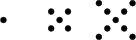
\includegraphics[width=\linewidth]{./images/x.png}
\end{image}%
\tcblower
\end{figureptx}%
\end{divisionexercise}%
\begin{divisionexercise}{3}{}{}{g:exercise:idp105544718371472}%
The first four terms in a sequence are listed below as numbers of dots. Determine a recursive description for the sequence. If possible, determine an explicit formula for the sequence.%
\begin{figureptx}{}{x:figure:fig-triangular-seq}{}%
\begin{image}{0}{1}{0}%

\includegraphics[width=\linewidth]{./images/triangular.png}
\end{image}%
\tcblower
\end{figureptx}%
\end{divisionexercise}%
\end{exercises-subsection-numberless}
\end{sectionptx}
%
%
\typeout{************************************************}
\typeout{Section 4.2 Discrete Dynamical Systems}
\typeout{************************************************}
%
\begin{sectionptx}{Discrete Dynamical Systems}{}{Discrete Dynamical Systems}{}{}{x:section:sec-dds}
\begin{assemblage}{Motivating Questions.}{g:assemblage:idp105544718373904}%
In this section, we will explore the following questions. %
\begin{enumerate}
\item{}What is a discrete dynamical system? How do they relate to sequences?%
\item{}How can we use discrete dynamical systems to describe real-world phenomena like predator-prey interactions, or the spread of a disease in a population?%
\end{enumerate}
%
\end{assemblage}
\begin{introduction}{}%
In \hyperref[x:section:sec-intro-to-dds]{Section~{\xreffont\ref{x:section:sec-intro-to-dds}}}, we introduced the notion of a sequence. In this section, we will focus on situations in which our sequences represent a quantity changing over discrete, consistent periods of time. We will also consider \emph{systems} of sequences: two or more interrelated sequences which describe the behavior of multiple changing quantities all at once. Before we dive into such systems, we consider another type of growth.%
\end{introduction}%
%
%
\typeout{************************************************}
\typeout{Subsection 4.2.1 Exponential Growth}
\typeout{************************************************}
%
\begin{subsectionptx}{Exponential Growth}{}{Exponential Growth}{}{}{x:subsection:subsec-exponential-growth}
Populations of people and animals do not grow linearly. Instead, they usually grow by a percentage of the whatever the current population is. So, if that percentage is, say, 10\%, and the current population of a group of fish in a pond is 1000, this model predicts a population of \(1000 + 10\%\cdot 1000 = 1000 + 100 = 1100\) fish for next year.%
\par
In symbols, if \(P_t\) represents the number of fish \(t\) years from now, then \(P_0 = 1000\), \(P_1 = P_0 + 0.1\cdot P_0 = (1+0.1)P_0 = 1.1 P_0\). The number 0.1 is called the \terminology{growth rate}, \(r\), and the number 1.1 is the \terminology{growth multiplier}.%
\par
In what follows, I will occasionally provide Sage cells in which you can do basic computations (and in which I may help get you started). To see how this works, click "Evaluate" in the Sage cell below to see what happens.%
\begin{sageinput}
P_0 = 1000
P_1 = 1.1*P_0
P_1
\end{sageinput}
\begin{exploration}{}{x:exploration:expl-exponential-growth}%
Consider a population of 1000 fish growing at 10\% per year.%
%
\begin{enumerate}
\item{}Give a formula for \(P_2\) in terms of \(P_1\), and then a formula for \(P_3\) in terms of \(P_2\).%
\item{}Using your answer to the previous part as a guide, give a formula for \(P_t\) in terms of \(P_{t-1}\).%
\item{}Again, using your answer to Question 1 and the work in the paragraph preceding this activity, give a formula for \(P_2\) in terms of \(P_0\). Use this formula to find \(P_3\) in terms of \(P_0\). Why might these formulas be more useful than the ones you found in Question 1?%
\item{}State your best guess for a formula for \(P_t\) in terms of \(P_0\). Use your formula to estimate the number of fish in the pond after 10, 20, and 50 years. What is this model missing?%
\item{}Press 'Evaluate' below to confirm your response to Question 4. What happens if you increase or decrease the growth rate, \(r\)? Try it, and reevaluate.%
\end{enumerate}
\begin{sageinput}
P_0 = 1000
r = 0.1
P(t) = (1+r)^t*P_0
tt = range(50)
PP = [P(t) for t in tt]
tP = list(zip(tt, PP))
P_dots = points(tP, color='red')
P_dots
\end{sageinput}
\end{exploration}%
The type of growth explored in \hyperref[x:exploration:expl-exponential-growth]{Exploration~{\xreffont\ref{x:exploration:expl-exponential-growth}}} called \terminology{exponential}, as the growth comes from taking the growth multiplier to larger and larger powers (exponents). We saw the danger of extrapolation with linear models in \hyperref[x:activity:act-linear-growth]{Activity~{\xreffont\ref{x:activity:act-linear-growth}}}, and we note a similar danger in extrapolating with exponential models. If nothing else, it's likely that the pond cannot \emph{hold} 100,000 fish. Thankfully, we can modify our exponential growth model by introducing an upper limit for what the habitat can hold.%
\begin{exploration}{}{x:exploration:expl-carrying-capacity}%
Suppose our pond can hold 5000 fish. This is known as the \emph{carrying capacity}, and we'll denote it with the letter \(K\)\begin{aside}{}{g:aside:idp105544718398480}%
\end{aside}
. We'll now let \(r = 0.1\) be our \emph{maximum} growth rate, but we'll let it slowly reduce as the population grows.%
%
\begin{enumerate}
\item{}As \(P_t\) increases and gets closer and closer to \(K\) over time, what happens to the ratio \(P_t/K\)? What number does it get close to?%
\item{}Thus, what happens to the expression \(1-\frac{P_t}{K}\) as \(P_t\) increases and gets closer and closer to \(K\)?%
\item{}Ecologically speaking, what does it mean for \(P_t\) to get closer and closer to \(K\)?%
\item{}As the phenomena described in Question 3 occurs, what do we expect the graph of \(P_t\) over time to look like?%
\item{}Test your suspicion by evaluating the Sage code below.%
\end{enumerate}
\begin{sageinput}
P_0=1000
r = 0.1
K = 5000
maxterm = 100
P(t)= K/(1+(K-P_0)/P_0*e^(-r*t))
tt = range(maxterm)
PP = [P(t) for t in tt]
tP = list(zip(tt, PP))
P_dots = points(tP, color='red')
P_dots
\end{sageinput}
\end{exploration}%
\end{subsectionptx}
%
%
\typeout{************************************************}
\typeout{Subsection 4.2.2 A discrete predator-prey model}
\typeout{************************************************}
%
\begin{subsectionptx}{A discrete predator-prey model}{}{A discrete predator-prey model}{}{}{g:subsection:idp105544718377232}
We now consider systems of discrete sequences, called \terminology{discrete dynamical systems}.%
\begin{definition}{}{x:definition:def-dynamical-system}%
A \terminology{dynamical system} refers to any fixed mathematical rule which describes how a system changes over time. A \terminology{discrete} dynamical system changes at fixed intervals in time (e.g., each hour), and does not change between the fixed points in time (e.g., a system that changes each hour will view the changing quantity as static between the hours of 1:00pm and 2:00pm).%
\end{definition}
There are two main types of dynamical systems: discrete and continuous. The study of continuous dynamical systems is the domain of calculus and its related disciplines (e.g., differential equations). Continuous dynamical systems treat time as infinitely divisible; discrete dynamical systems do not. Typically, a dynamical \emph{system} involves multiple related quantities that change over time.%
\par
We begin with a classic predator-prey model adapted from the \href{https://www.cds.caltech.edu/\~murray/amwiki/index.php/Predator_prey}{Feedback Systems Wiki}\footnote{\nolinkurl{https://www.cds.caltech.edu/\~murray/amwiki/index.php/Predator_prey}\label{g:fn:idp105544718381200}} at Caltech. For historical reasons, we let \(L_t\) be the size of a population of Canadian lynxes in year \(t\) and \(H_t\) be the size of a population of snowshoe hares, the lynx's primary prey. \begin{aside}{}{g:aside:idp105544718382736}%
\end{aside}
%
\begin{definition}{}{x:definition:def-lotkavolterra}%
Let \(H_0\) be the initial population of hares, and \(L_0\) the initial population of lynxes. For \(t\ge 1\), the \terminology{discrete Lotka-Volterra model} for the lynx\slash{}hare population is given by:%
%
\begin{align*}
H_{t+1} \amp = H_t + b(u) H_t - a L_t H_t\\
L_{t+1} \amp = L_t + c L_t H_t - d L_t,
\end{align*}
where \(b\) is the hare birth rate per unit time as a function of the food supply \(u\), \(d\) is the lynx mortality rate, and \(a\) and \(c\) are interaction coefficients.%
\end{definition}
Note the interrelationship between the two equations: the formula for calculating \(H_{t+1}\) requires knowing not only \(H_t\), but also \(L_t\). This makes sense! These populations interact, so the presence (or absence) of lynx should reasonably affect the hare population. Let's further analyze this model.%
\begin{exploration}{}{g:exploration:idp105544718389392}%
Consider the predator\slash{}prey model introduced in \hyperref[x:definition:def-lotkavolterra]{Definition~{\xreffont\ref{x:definition:def-lotkavolterra}}}.%
%
\begin{enumerate}
\item{}What do the terms \(L_t\) and \(H_t\) represent?%
\item{}Which term in the model represents an increase in the hare population? Which term represents a decrease in the hare population? Explain how you know.%
\item{}Which term in the model represents an increase in the lynx population? Which term represents a decrease in the lynx population? Explain how you know.%
\item{}What does the product \(L_t H_t\) represent? (The \href{https://en.wikipedia.org/wiki/Rule_of_product}{multiplication principle}\footnotemark{} may be helpful here; also consider what \(a\) is described to be.)%
\item{}What simplifying assumptions does this model make about how the populations increase and decrease?%
\end{enumerate}
\end{exploration}%
\footnotetext[2]{\nolinkurl{https://en.wikipedia.org/wiki/Rule_of_product}\label{g:fn:idp105544718426000}}%
\begin{activity}{}{g:activity:idp105544718427024}%
Let's start by assuming that \(H_0 = 20\) and \(L_0 = 35\). That is, we begin with 20 hares and 35 lynxes. Let's further assume that \(a = c = 0.001167\), \(b = 0.05\), and \(d = 0.0583\) (parameters scaled by 12 months).%
%
\begin{enumerate}
\item{}Compute \(H_1, H_2, L_1,\) and \(L_2\). What seems to be happening to the two populations? Confirm using the Sage cell below, which will display the first ten months' worth of predictions, or explore \href{https://docs.google.com/spreadsheets/d/1sFOHJ-LNA39Ydj_GDg69XhtNwWVtpWNweBT5IBzjJGo/edit?usp=sharing}{this spreadsheet}\footnotemark{}. Note that the hare population is given by the blue dots and the lynx population by the red. \begin{sageinput}
H_0 = 10 # This is the initial hare population
L_0 = 10 # This is the initial lynx population
a = 0.014 # This represents the predation rate
b=0.6 # Growth rate of hares
c=a # This represents the predation rate
d=0.7 # death rate of lynx
nperiod = 12 # number of time periods in a year
def H(n):
	if n==0:
		return H_0
	else:
		return H(n-1) + (b*H(n-1)-a*L(n-1)*H(n-1))/nperiod

def L(n):
	if n==0:
		return L_0
	else:
		return L(n-1) + c*L(n-1)*H(n-1)-(d*L(n-1))/nperiod
time=10
nn=range(time)
HH = [H(n) for n in nn]
LL = [L(n) for n in nn]
nH = list(zip(nn, HH))
nL = list(zip(nn, LL))
H_dots = points(nH, color='blue')
L_dots = points(nL, color='red')
p = H_dots + L_dots
p
\end{sageinput}
%
\item{}The interaction coefficients translate to a decrease in the lynx population and an increase in the hare population. What do you expect to happen if we increase it from 0.014 to 0.05?%
\item{}Test your suspicion using the Sage cell below, or \href{https://docs.google.com/spreadsheets/d/1sFOHJ-LNA39Ydj_GDg69XhtNwWVtpWNweBT5IBzjJGo/edit?usp=sharing}{this spreadsheet}\footnotemark{}. \begin{sageinput}
H_0 = 10 # This is the initial hare population
L_0 = 10 # This is the initial lynx population
a = 0.05 # This represents the predation rate
b=0.6 # Growth rate of hares
c=a # This represents the predation rate
d=0.7 # death rate of lynx
nperiod=12
def H(n):
	if n==0:
		return H_0
	else:
		return H(n-1) + (b*H(n-1)-a*L(n-1)*H(n-1))/nperiod

def L(n):
	if n==0:
		return L_0
	else:
		return L(n-1) + (c*L(n-1)*H(n-1)-d*L(n-1))/nperiod
time=10
nn=range(time)
HH = [H(n) for n in nn]
LL = [L(n) for n in nn]
nH = list(zip(nn, HH))
nL = list(zip(nn, LL))
H_dots = points(nH, color='blue')
L_dots = points(nL, color='red')
p = H_dots + L_dots
p
\end{sageinput}
%
\item{}Qualitatively describe the dynamics displayed in the Sage output in the previous question.%
\end{enumerate}
\end{activity}%
\footnotetext[3]{\nolinkurl{https://docs.google.com/spreadsheets/d/1sFOHJ-LNA39Ydj_GDg69XhtNwWVtpWNweBT5IBzjJGo/edit?usp=sharing}\label{g:fn:idp105544718431248}}%
\footnotetext[4]{\nolinkurl{https://docs.google.com/spreadsheets/d/1sFOHJ-LNA39Ydj_GDg69XhtNwWVtpWNweBT5IBzjJGo/edit?usp=sharing}\label{g:fn:idp105544718433040}}%
One might reasonably wonder how such a simple model does in making predictions about the long-term dynamics of these populations. The answer is: surprisingly well! In \hyperref[x:figure:fig-harelynxdata]{Figure~{\xreffont\ref{x:figure:fig-harelynxdata}}}, observe the actual collected data on hare and lynx populations over 90 years, from 1845 to 1935. In \hyperref[x:figure:fig-harelynxmodel]{Figure~{\xreffont\ref{x:figure:fig-harelynxmodel}}}, we see dynamics predicted by the model. Note the same cyclical patterns of an increase in the hare population followed by an increase in the lynx population, which in turn causes a decrease in the hare population, etc.%
\begin{figureptx}{Data on hare and lynx populations over time. (\href{https://www.cds.caltech.edu/\~murray/amwiki/index.php/Predator_prey}{Source}\protect\footnotemark{})}{x:figure:fig-harelynxdata}{}%
\begin{image}{0.25}{0.5}{0.25}%
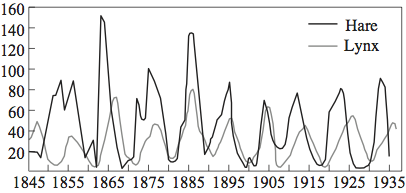
\includegraphics[width=\linewidth]{https://www.cds.caltech.edu/~murray/amwiki/images/0/08/Predprey-graph.png}
\end{image}%
\tcblower
\end{figureptx}%
\footnotetext[5]{\nolinkurl{https://www.cds.caltech.edu/\~murray/amwiki/index.php/Predator_prey}\label{g:fn:idp105544718436368}}%
\begin{figureptx}{The predicted dynamics of hare and lynx populations over time. (\href{https://www.cds.caltech.edu/\~murray/amwiki/index.php/Predator_prey}{Source}\protect\footnotemark{})}{x:figure:fig-harelynxmodel}{}%
\begin{image}{0.25}{0.5}{0.25}%
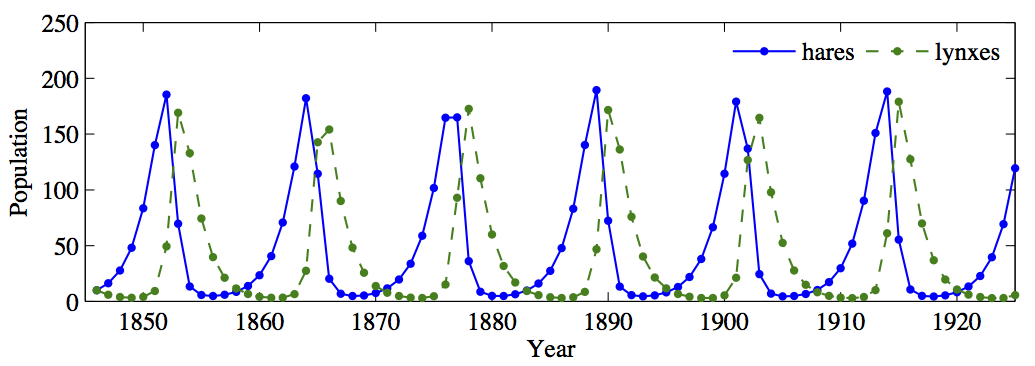
\includegraphics[width=\linewidth]{https://www.cds.caltech.edu/~murray/amwiki/images/9/9a/Predprey-discrete.png}
\end{image}%
\tcblower
\end{figureptx}%
\footnotetext[6]{\nolinkurl{https://www.cds.caltech.edu/\~murray/amwiki/index.php/Predator_prey}\label{g:fn:idp105544718438160}}%
To be clear, the purpose of the model is not to make absolutely certain predictions about the precise numbers of hares and lynxes present in the Canadian wilderness. Instead, we want to understand the broad dynamics of how the populations change relative to one another. Mathematical ecologists can then use these models to understand how small changes in the parameters (say, an increase in the rate of predation) affect the broader dynamics of the ecological system.%
\end{subsectionptx}
%
%
\typeout{************************************************}
\typeout{Subsection 4.2.3 The discrete SIR epidemiological model}
\typeout{************************************************}
%
\begin{subsectionptx}{The discrete SIR epidemiological model}{}{The discrete SIR epidemiological model}{}{}{g:subsection:idp105544718439312}
We now arrive at the main focus of this two-week unit: a basic mathematical model for the spread of an infectious disease. We'll first present the model itself and examine its features and assumptions. As was the case with the predator-prey model, we'll see that while it does make simplifying assumptions, it still allows us to analyze the broader dynamics of the disease transmission. We'll then look at ways of reducing the rate of infection, including the so-called "flattening the curve" method.%
\par
We begin with the model. It is known as a \emph{compartmental model}, as it divides the population into compartments and assumes that every individual in the same compartment has the same characteristics (at least as far as the transmission of the disease is concerned). We'll look at the simplest such model, the discrete SIR model. Many more complex models are built on the SIR model.%
\begin{definition}{}{g:definition:idp105544718408208}%
Consider a population of \(N\) people through which a disease is spreading. For some discrete time \(t \ge 0\), let \(S_t\) denote the number of individuals \emph{susceptible} to the disease, \(I_t\) the number of individuals \emph{infected} with the disease, and \(R_t\) the number of individuals who have \emph{recovered} from the disease. We assume that that people move through the compartments as follows:%
%
\begin{equation}
S \to I \to R.\label{x:men:eq-compartments}
\end{equation}
For \(t\ge 1\), the model is given by the following equations.%
%
\begin{align*}
N \amp = S_t + I_t + R_t\\
S_{t+1} \amp = S_t -b S_t I_t\\
I_{t+1} \amp = I_t + b S_t I_t - a I_t\\
R_{t+1} \amp = R_t + a I_t.
\end{align*}
The constant \(a\) is known as the \emph{recovery rate} parameter, which roughly describes how fast someone moves from the infected compartment to the recovered compartment. The constant \(b\) is known as the \emph{infection rate}, and roughly describes how fast someone moves from the susceptible compartment to the infected compartment.%
\end{definition}
Let's explore the equations.%
\begin{exploration}{}{g:exploration:idp105544718416016}%
%
\begin{enumerate}
\item{}What does \hyperref[x:men:eq-compartments]{({\xreffont\ref{x:men:eq-compartments}})} mean? What assumptions does this make? How does it simplify our analysis?%
\item{}What does the first equation in the set of four mean? What assumptions does it make about the population?%
\item{}The second equation describes how the susceptible population changes over time. It contains the term \(-b S_t I_t\). Based on our work above with a predator-prey model and the definition of \(b\), what epidemiological event is this term describing?%
\item{}Explain why it makes sense that we add \(b S_t I_t\) in the equation defining \(I_{t+1}\).%
\item{}What does the term \(-a I_t\) mean in the equation for \(I_{t+1}\)? Why does it make sense to \emph{add} \(a I_t\) in the equation for \(R_{t+1}\)?%
\item{}Note that there are no terms being subtracted in the equation for \(R_{t+1}\). What assumption does this tell us that the model is making?%
\end{enumerate}
\end{exploration}%
\begin{activity}{}{x:activity:act-sirnumbers}%
Let's see what happens when we plug in some numbers. Assume that \(N = 10,000\), \(R_0 = 0\), and \(I_0 = 50\).%
%
\begin{enumerate}
\item{}Why does it make sense that we have \(R_0 = 0\) (assuming we have a new disease entering a population).%
\item{}What is \(S_0\)?%
\item{}Let's assume that \(a = 0.1\) and \(b = 0.0001\). Compute \(S_1, I_1\), and \(R_1\).%
\item{}Use your answer to the previous part to compute \(S_2, I_2\), and \(R_2\).%
\item{}Now check your work using \href{https://docs.google.com/spreadsheets/d/153LO2O21_TwEYyODq2Km90oRrilLEpfYmgb8w3AJSQo/edit?usp=sharing}{this spreadsheet}\footnotemark{} (download a copy to your device and edit it there).%
\end{enumerate}
\end{activity}%
\footnotetext[7]{\nolinkurl{https://docs.google.com/spreadsheets/d/153LO2O21_TwEYyODq2Km90oRrilLEpfYmgb8w3AJSQo/edit?usp=sharing}\label{g:fn:idp105544718462096}}%
\begin{investigation}{}{g:investigation:idp105544718462480}%
In this and the following activity, we'll use the spreadsheet \href{https://docs.google.com/spreadsheets/d/153LO2O21_TwEYyODq2Km90oRrilLEpfYmgb8w3AJSQo/edit?usp=sharing}{found here}\footnotemark{}. Download the file and play around with the numbers at the top of the sheet to change some of the features; e.g., how does increasing\slash{}decreasing the number of initial infected individuals change the shape of the curves? What do you notice? What do you wonder? Give at least 2-3 observations or questions.%
\end{investigation}%
\footnotetext[8]{\nolinkurl{https://docs.google.com/spreadsheets/d/153LO2O21_TwEYyODq2Km90oRrilLEpfYmgb8w3AJSQo/edit?usp=sharing}\label{g:fn:idp105544718463632}}%
The COVID-19 pandemic introduced many people to a quantity called \(r_0\). \begin{aside}{}{g:aside:idp105544718464656}%
\end{aside}
 This is known as the \terminology{basic reproduction number}, and is the expected number of new infections \emph{directly generated} by a single case. So, if I were to get COVID-19, \(r_0\) would be the expected number of people I would \emph{directly} infect. We would then expect each of \emph{them} to infect another \(r_0\) people, and so on.%
\par
Generally, if \(r_0 \gt 1\), we expect the disease to spread. If \(r_0 \lt 1\), we expect it to die out.%
\par
The next activity explores the ways in which varying \(r_0\) impacts new cases of the disease caused both directly and indirectly by a single person.%
\begin{activity}{}{x:activity:act-r0}%
In this activity, we assume different values for \(r_0\). However, we will make two assumptions that don't change.%
\par
First, assume that all direct infections are done within a 5-day period. Second, assume that that those infected don't infect others until the next five day period.%
\par
Let \(C_t\) be the number of cases I've caused after \(t\) five-day periods. Assume \(C_0 = 1\) (me).%
%
\begin{enumerate}
\item{}Explain why \(C_1 = r_0 C_0 = r_0\).%
\item{}Explain why \(C_2 = C_1 + r_0 C_1 = r_0 + r_0^2\).%
\item{}After 30 days, six five-day periods will have passed. Explain why%
\begin{equation*}
C_6 = r_0 + r_0^2 + r_0^3 + \cdots + r_0^6.
\end{equation*}
%
\item{}Our SIR model approximates \(r_0\) by the formula%
\begin{equation}
r_0 \approx \frac{bN}{a}.\label{x:men:eq-r0}
\end{equation}
Using that formula, what is the approximate \(r_0\) for the situation described in \hyperref[x:activity:act-sirnumbers]{Activity~{\xreffont\ref{x:activity:act-sirnumbers}}}?%
\item{}Given that value of \(r_0\), use the Sage cell below (replacing the ? with the value you found) to estimate how many cases I am responsible for over a 30-day period.%
\item{}The practice of \href{https://en.wikipedia.org/wiki/Social_distancing}{social distancing}\footnotemark{} is intended to reduce \(r_0\). Assume that strict social distancing is observed, and this reduces \(r_0\) to approximately 1.25 (one direct infection fewer). Now how many cases are you responsible for over the course of a 30-day period?%
\item{}As the COVID-19 situation is ongoing, estimates for \(r_0\) vary significantly. \href{https://academic.oup.com/jtm/article/27/2/taaa021/5735319}{One study from February 2020}\footnotemark{} found an average \(r_0\) of 3.28. If that is the true number, approximately how many cases will a typical infected person be responsible for over the course of a month? Use the Sage cell to determine your answer.%
\item{}Other studies suggest that, in the absence of any social interventions, the COVID-19 has \(r_0 \approx 2.38\). In that case, how many cases would an infected person be responsible for over the course of a month?%
\item{}The Delta variant of COVID-19 has a \(r_0 \approx 5.1\). If I am infected with the Delta variant, approximately how many new cases will I cause within a month?%
\item{}The Omicron variant of COVID-19 has an estimated \(r_0 \approx 10\)\footnotemark{}. If I am infected with the Omicron variant, approximately how many new cases will I cause within a month?%
\end{enumerate}
\begin{sageinput}
r_0 = ?
r_0 + r_0^2 + r_0^3 + r_0^4 + r_0^5 + r_0^6
\end{sageinput}
\end{activity}%
\footnotetext[9]{\nolinkurl{https://en.wikipedia.org/wiki/Social_distancing}\label{g:fn:idp105544718444304}}%
\footnotetext[10]{\nolinkurl{https://academic.oup.com/jtm/article/27/2/taaa021/5735319}\label{g:fn:idp105544718446480}}%
\footnotetext[11]{This is being written in February 2022, just as the first major Omicron wave is subsiding; it should therefore be treated as preliminary.\label{g:fn:idp105544718449040}}%
For our last activity, we'll explore how reducing \(r_0\) "flattens" the curve of infected people at time \(t\), \(I_t\). There are two main advantages of a flattened infected curve. First, this often corresponds to fewer infected people overall. Second, the lack of a spike in infected persons makes it easier for the healthcare system to effectively treat those who \emph{are} infected (not to mention anyone with other medical concerns).%
\begin{exploration}{}{g:exploration:idp105544718451600}%
One last time, consider the values for the variables we used in \hyperref[x:activity:act-sirnumbers]{Activity~{\xreffont\ref{x:activity:act-sirnumbers}}}; for reference, this was \(S_0 = 10000\), \(I_0 = 50\), \(R_0 = 0\), \(a = 0.1\), and \(b = 0.0001\). We'll again use the \href{https://drive.google.com/file/d/1xSJ6KM8x9HVdo9-P4QoUOoSmmfpKmmIQ/view?usp=sharing}{Google sheet}\footnotemark{} to answer these questions.%
%
\begin{enumerate}
\item{}What is \(r_0\)? (Recall \hyperref[x:men:eq-r0]{({\xreffont\ref{x:men:eq-r0}})} from Question 4 of \hyperref[x:activity:act-r0]{Activity~{\xreffont\ref{x:activity:act-r0}}}.)%
\item{}This value is pretty high (though it is approximately the \(r_0\) of diseases like measles and chicken pox!), but is convenient for our purposes. Nonetheless, we can still explore the ways in which changes in \(r_0\) affect the shape of the curves; our qualitative observations will still apply to real-world situations like the current coronavirus pandemic.%
\par
Recall that \(r_0 \approx \frac{bN}{a}\) and assume our population size \(N = 10000\) and recovery rate \(a = 0.1\) are constant. Compute the three values of \(r_0\) that result from infection rates of \(b = 0.00005, 0.0001\), and \(0.0002\). In turn, plug these values into the \href{https://drive.google.com/file/d/1xSJ6KM8x9HVdo9-P4QoUOoSmmfpKmmIQ/view?usp=sharing}{Google sheet}\footnotemark{} and comment on the shape of the infection curve: how tall is the spike of infected individuals, and at what time \(t\) is it at its highest point?%
\item{}Similarly, assuming \(N = 10000\) and \(b = 0.0001\) are constant, compute the values of \(r_0\) that result from \(a = 0.05, 0.1\), and \(0.2\). In turn, plug these values into the \href{https://drive.google.com/file/d/1xSJ6KM8x9HVdo9-P4QoUOoSmmfpKmmIQ/view?usp=sharing}{Google sheet}\footnotemark{} and comment on the shape of the (green) infection curve: how tall is the spike of infected individuals, and at what time \(t\) is it at its highest point?%
\end{enumerate}
\end{exploration}%
\footnotetext[12]{\nolinkurl{https://drive.google.com/file/d/1xSJ6KM8x9HVdo9-P4QoUOoSmmfpKmmIQ/view?usp=sharing}\label{g:fn:idp105544718455056}}%
\footnotetext[13]{\nolinkurl{https://drive.google.com/file/d/1xSJ6KM8x9HVdo9-P4QoUOoSmmfpKmmIQ/view?usp=sharing}\label{g:fn:idp105544718231824}}%
\footnotetext[14]{\nolinkurl{https://drive.google.com/file/d/1xSJ6KM8x9HVdo9-P4QoUOoSmmfpKmmIQ/view?usp=sharing}\label{g:fn:idp105544718235280}}%
\end{subsectionptx}
\end{sectionptx}
\end{chapterptx}
 %
%
\typeout{************************************************}
\typeout{Chapter 5 Graphs}
\typeout{************************************************}
%
\begin{chapterptx}{Graphs}{}{Graphs}{}{}{x:chapter:chap-graphs}
%
%
\typeout{************************************************}
\typeout{Section 5.1 Intro to Graph Theory}
\typeout{************************************************}
%
\begin{sectionptx}{Intro to Graph Theory}{}{Intro to Graph Theory}{}{}{x:section:sec-intro-gt}
%
%
\typeout{************************************************}
\typeout{Subsection 5.1.1 The Bridges of Konigsberg}
\typeout{************************************************}
%
\begin{subsectionptx}{The Bridges of Konigsberg}{}{The Bridges of Konigsberg}{}{}{g:subsection:idp105544718238096}
\begin{investigation}{}{p:investigation:dGT}%
\index{Seven Bridges of Königsberg}%
\index{Königsberg, Seven Bridges of}%
\index{puzzle!seven bridges}%
\index{Seven Bridges of Königsberg}%
\index{Königsberg, Seven Bridges of}%
\index{puzzle!seven bridges}%
In the town of Königsberg in Prussia, there was a river containing two islands. The islands were connected to the banks of the river by seven bridges (as seen below). On their days off, townspeople would play a little game with themselves as they walked over the bridges: was it possible to plan a walk so that you cross each bridge once and only once?%
\begin{sidebyside}{1}{0.1}{0.1}{0}%
\begin{sbspanel}{0.8}%
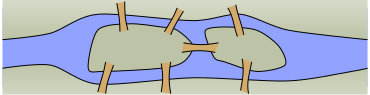
\includegraphics[width=\linewidth]{./images/gt-bridges-art.png}
\end{sbspanel}%
\end{sidebyside}%
\end{investigation}%
\end{subsectionptx}
%
%
\typeout{************************************************}
\typeout{Subsection 5.1.2 Background and terminology}
\typeout{************************************************}
%
\begin{subsectionptx}{Background and terminology}{}{Background and terminology}{}{}{g:subsection:idp105544718242064}
You've almost certainly encountered the word \emph{graph} in a math class.%
\begin{principle}{}{}{g:principle:idp105544718243472}%
What is meant by the word \emph{graph} in a mathematical context? Give as many answers as you can, and be as clear and precise as possible.%
\end{principle}
A relatively new (by mathematical standards) use of the word \emph{graph} in mathematics involves the notion of connection. It is this notion that we will be exploring in this unit. We present a formal definition below.%
\begin{definition}{}{g:definition:idp105544718212240}%
A \terminology{graph}, \(G\), is a collection of \terminology{vertices} (or \terminology{nodes}), \(V\), and a collection of edges, \(E\), which are pairs of vertices. We denote the graph as \(G(V,E)\).%
\end{definition}
This relatively simple, short definition nonetheless has deep consequences. We'll see an example below, but note that the primary defining features of a graph \(G\) are some objects (vertices) and the connections between (some of) the objects (the edges). If a vertex \(v\) is connected to another vertex \(u\) by an edge \(vu\), we say \(uv\) is \terminology{incident} to \(v\), and we say \(u\) is \terminology{adjacent} to \(v\) and is in the \terminology{neighborhood} of \(v\).%
\begin{example}{}{g:example:idp105544718220304}%
As a straightforward initial example, consider the graph \(G(V, E)\) where \(V = \{a,b,c,d\}\) and \(E = \{ab,ac,bd\}\). This graph has four vertices, and three edges. One \terminology{representation} (drawing) of it is given in \hyperref[x:figure:fig-graphexample1]{Figure~{\xreffont\ref{x:figure:fig-graphexample1}}}. \begin{figureptx}{One (bad) drawing of \(G\).}{x:figure:fig-graphexample1}{}%
\begin{image}{0.25}{0.5}{0.25}%
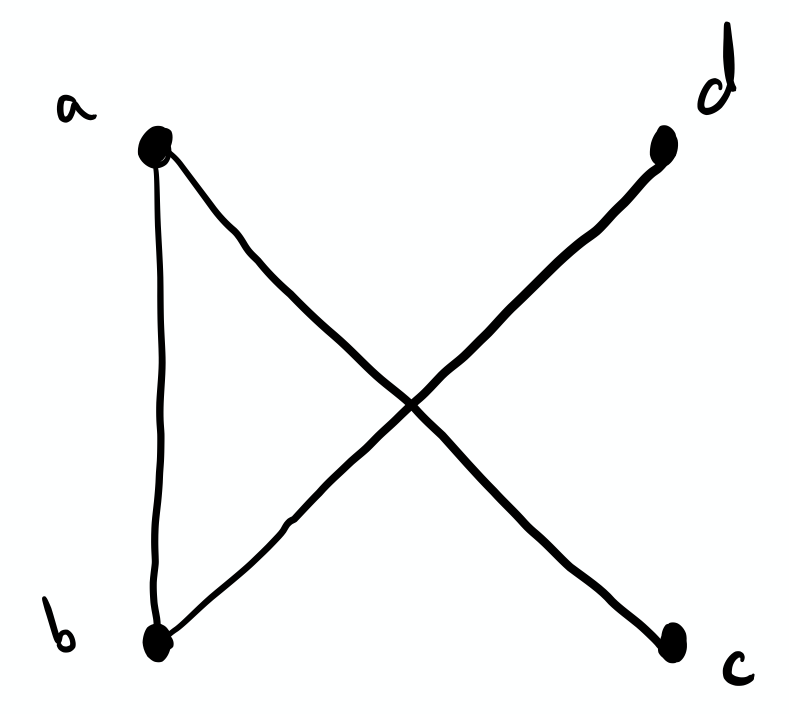
\includegraphics[width=\linewidth]{images/graph01.png}
\end{image}%
\tcblower
\end{figureptx}%
 As stated above, the most important feature of a graph is the connections it describes. Thus, we would say the graph in \hyperref[x:figure:fig-graphexample2]{Figure~{\xreffont\ref{x:figure:fig-graphexample2}}} \emph{also} represents the graph \(G\) from \hyperref[x:figure:fig-graphexample1]{Figure~{\xreffont\ref{x:figure:fig-graphexample1}}}. \begin{figureptx}{Another (bad) drawing of \(G\).}{x:figure:fig-graphexample2}{}%
\begin{image}{0.25}{0.5}{0.25}%
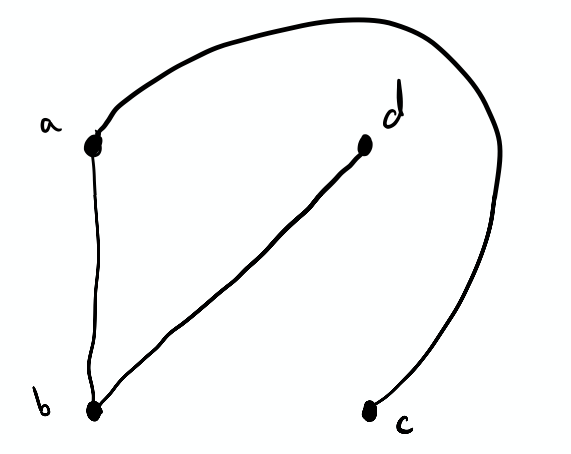
\includegraphics[width=\linewidth]{images/graph02.png}
\end{image}%
\tcblower
\end{figureptx}%
%
\end{example}
\begin{activity}{}{g:activity:idp105544718259984}%
In this activity, your job is to invent a graph \(G\) with the following properties. Draw it and be ready to share it. Then explain why your example meets the given criteria (e.g., for Question 4, which vertex has at least three neighbors?).%
%
\begin{enumerate}
\item{}Your graph should have six vertices%
\item{}Your graph should have ten edges%
\item{}There should be at least one pair of vertices between which you cannot trace a path of edges%
\item{}One vertex should should have at least three others in its neighborhood%
\end{enumerate}
\end{activity}%
\begin{exploration}{}{g:exploration:idp105544718262288}%
We saw in the last unit that we could model changing quantities over time using discrete dynamical systems. Graphs, on the other hand, describe connections between objects. Brainstorm or research at least two or three complex, real-world situations which graphs might be helpful to model. That is, can you think of at least two or three situations in which one of the fundamental properties is \emph{connection}? Briefly describe each situation in 3-4 sentences, and make clear how graphs can be used to describe these situations. If you find examples of such graphs, be ready to share.%
\end{exploration}%
In order to discuss the nuances of the connections modeled by a graph, we need a bit more terminology.%
\begin{definition}{}{x:definition:def-deg}%
Let \(G(V,E)\) be a graph. A vertex \(v\) in \(V\) is \terminology{isolated} if it has no neighbors. The number of edges incident to a vertex \(v\) is known as the \terminology{degree} of \(v\), denoted \(\deg(v)\). If between every pair of vertices in \(V\) there is a path of edges, we say \(G\) is \terminology{connected}. Otherwise, we say \(G\) is not connected. Each of the largest possible connected pieces of \(G\) is known as a \terminology{component} of \(G\).%
\end{definition}
\begin{exploration}{}{g:exploration:idp105544718270096}%
For this exploration, we will consider the graph \(G(V,E)\) in \hyperref[x:figure:fig-graphexample3]{Figure~{\xreffont\ref{x:figure:fig-graphexample3}}}.%
\begin{figureptx}{A graph \(G\).}{x:figure:fig-graphexample3}{}%
\begin{image}{0.25}{0.5}{0.25}%
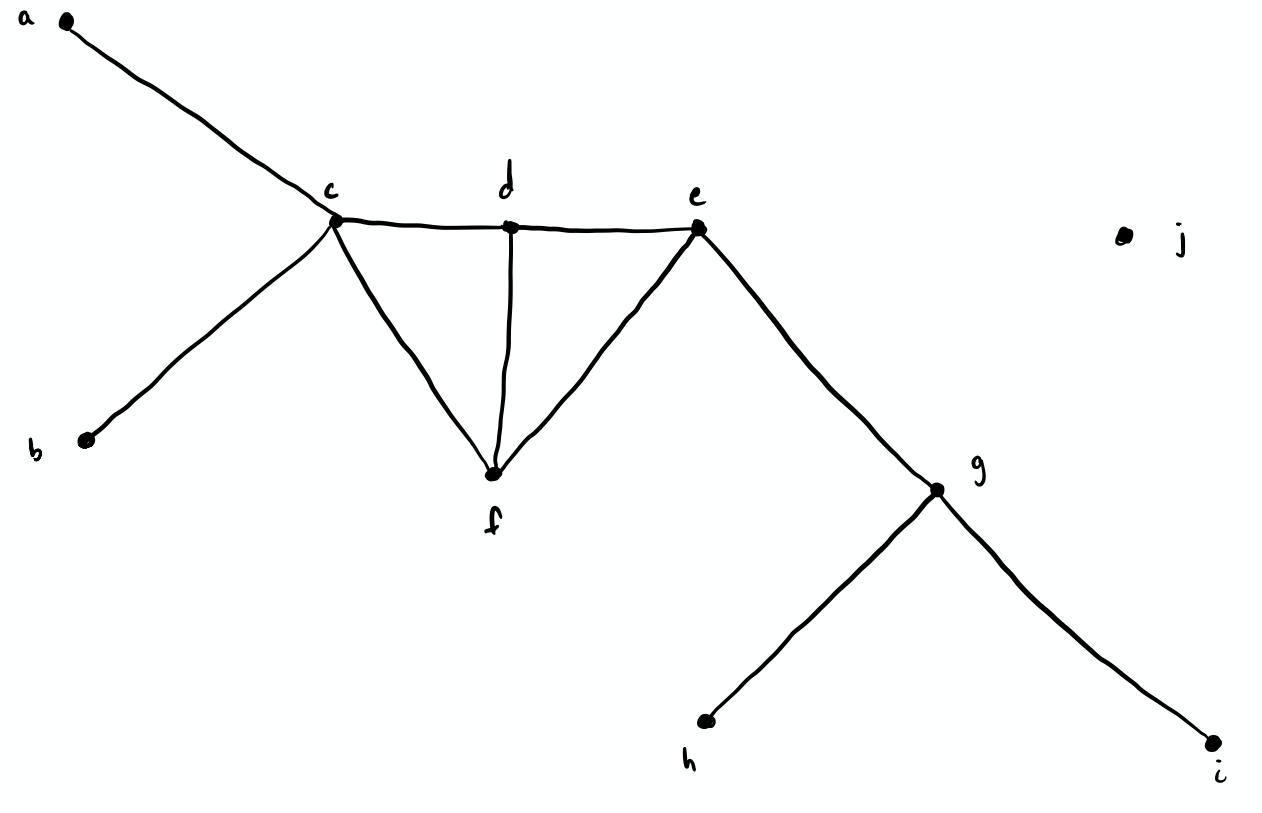
\includegraphics[width=\linewidth]{images/graph03.png}
\end{image}%
\tcblower
\end{figureptx}%
%
\begin{enumerate}
\item{}Is \(G\) connected? How many components does it have?%
\item{}Does \(G\) have any isolated vertices? If so, what are their degrees?%
\item{}What is the largest degree of a vertex in \(G\)? Which vertex\slash{}vertices have that degree?%
\item{}Suppose that \(G\) represents a social network; that is, the vertices represent people, and the edges represent friendship. Who are \(e\)'s friends?%
\item{}Still viewing \(G\) as the model of a network of friends, which pair of people do you think are more likely to become friends next: \(a\) and \(b\), or \(c\) and \(e\)? Why?%
\item{}Still viewing \(G\) as the model of a network of friends, which pair of people do you think are more likely to become friends next: \(a\) and \(b\), or \(c\) and \(h\)? Why?%
\end{enumerate}
\end{exploration}%
Next time, we'll explore the underlying structure of connectedness in graphs in more depth. In particular, we'll search for minimal (in terms of numbers of edges) subgraphs called \emph{trees} to help us see which edges are most important.%
\end{subsectionptx}
\end{sectionptx}
%
%
\typeout{************************************************}
\typeout{Section 5.2 April 9: Planar Graphs}
\typeout{************************************************}
%
\begin{sectionptx}{April 9: Planar Graphs}{}{April 9: Planar Graphs}{}{}{x:section:sec-planar-graphs}
\begin{exploration}{}{g:exploration:idp105544718249616}%
Let's look at the utilities problem and the model train problem.%
\end{exploration}%
The two graphs you drew above are famous and have special names: the first is the \terminology{complete bipartite graph \(K_{3,3}\)}, because you can group the vertices into two parts (``bi-partite'') such that every vertex from one group is connected to every vertex in the other. The second is called the \terminology{complete graph on five vertices, \(K_5\)}, because it contains all possible edges connecting the vertices.%
\begin{activity}{}{g:activity:idp105544718252304}%
Find at least two different drawings each of the graphs \(K_{3,3}\) and \(K_5\). If possible, try to find drawings of the graphs which solve the original problems. Note that your different drawings still describe the same connections.%
\end{activity}%
\begin{definition}{}{g:definition:idp105544718253840}%
A graph is called \terminology{planar} if it is \emph{possible} to draw the graph in such a way that none of the edges cross.%
\end{definition}
\begin{exploration}{}{g:exploration:idp105544718255120}%
Consider the graphs below. For each graph, determine whether it is planar. If so, draw it so none of the edges cross. If not, explain why not.%
\begin{figureptx}{}{x:figure:fig-planarity}{}%
\begin{image}{0.175}{0.65}{0.175}%
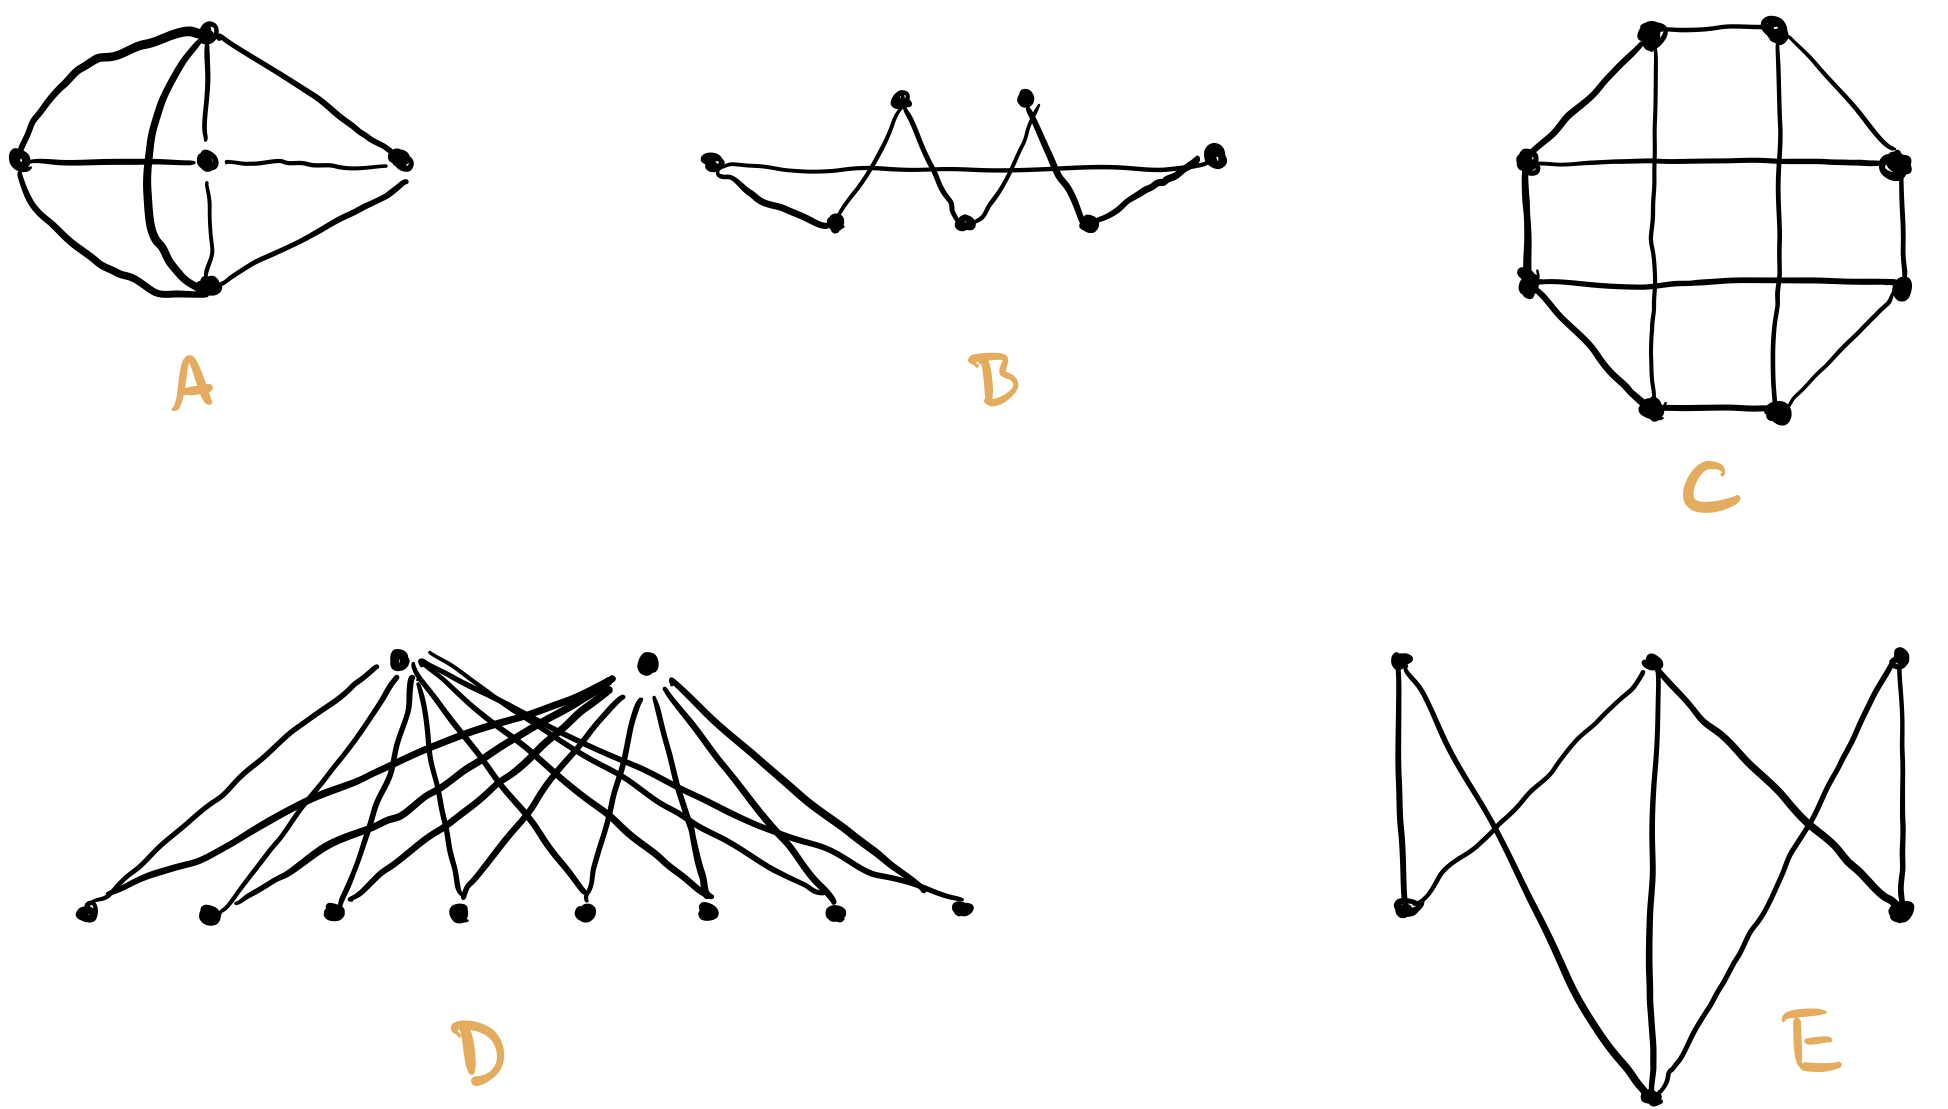
\includegraphics[width=\linewidth]{./images/planarity.png}
\end{image}%
\tcblower
\end{figureptx}%
\end{exploration}%
Thus, the utilities and model train problems can be stated as follows: Are \(K_{3,3}\) or \(K_5\) planar?%
\begin{theorem}{}{}{g:theorem:idp105544718257552}%
A graph is planar if and only if it does not contain a copy of \(K_{3,3}\) or \(K_5\), or a \terminology{subdivision} of \(K_{3,3}\) or  \(K_5\).\end{theorem}
\begin{exploration}{}{g:exploration:idp105544718292880}%
To see what we mean by ``subdivision'', is the following graph planar?%
\begin{figureptx}{}{x:figure:fig-subdivision}{}%
\begin{image}{0.25}{0.5}{0.25}%
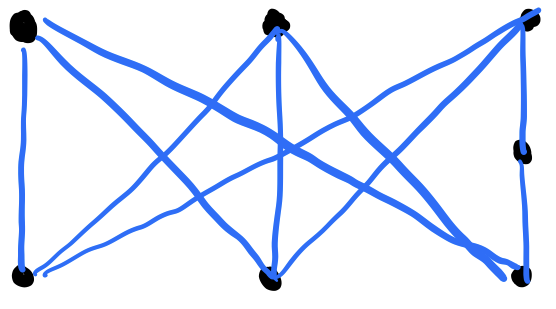
\includegraphics[width=\linewidth]{./images/subdivision.png}
\end{image}%
\tcblower
\end{figureptx}%
\end{exploration}%
\end{sectionptx}
%
%
\typeout{************************************************}
\typeout{Section 5.3 Apr. 12: Graph Coloring}
\typeout{************************************************}
%
\begin{sectionptx}{Apr. 12: Graph Coloring}{}{Apr. 12: Graph Coloring}{}{}{x:section:sec-graph-coloring}
Another application of planar graphs arises when deciding how to color a map. A useful coloring must not color states that share a common border (that is, a part of their boundary) with the same color (otherwise it’s difficult to tell where one starts and another begins!). However, an efficient mapmaker might wonder how many colors are needed to color any world map so that no countries which share a border are given the same color.%
\begin{exploration}{}{g:exploration:idp105544718295824}%
Consider the \href{./usa_map.pdf}{blank map of the USA}\footnotemark{} displayed in \hyperref[x:figure:fig-usa-map]{Figure~{\xreffont\ref{x:figure:fig-usa-map}}}. How many different colors are \emph{needed} in order to color the states so that no states that share a border are given the same color? How could we model this problem with a graph?%
\begin{figureptx}{}{x:figure:fig-usa-map}{}%
\begin{image}{0.175}{0.65}{0.175}%
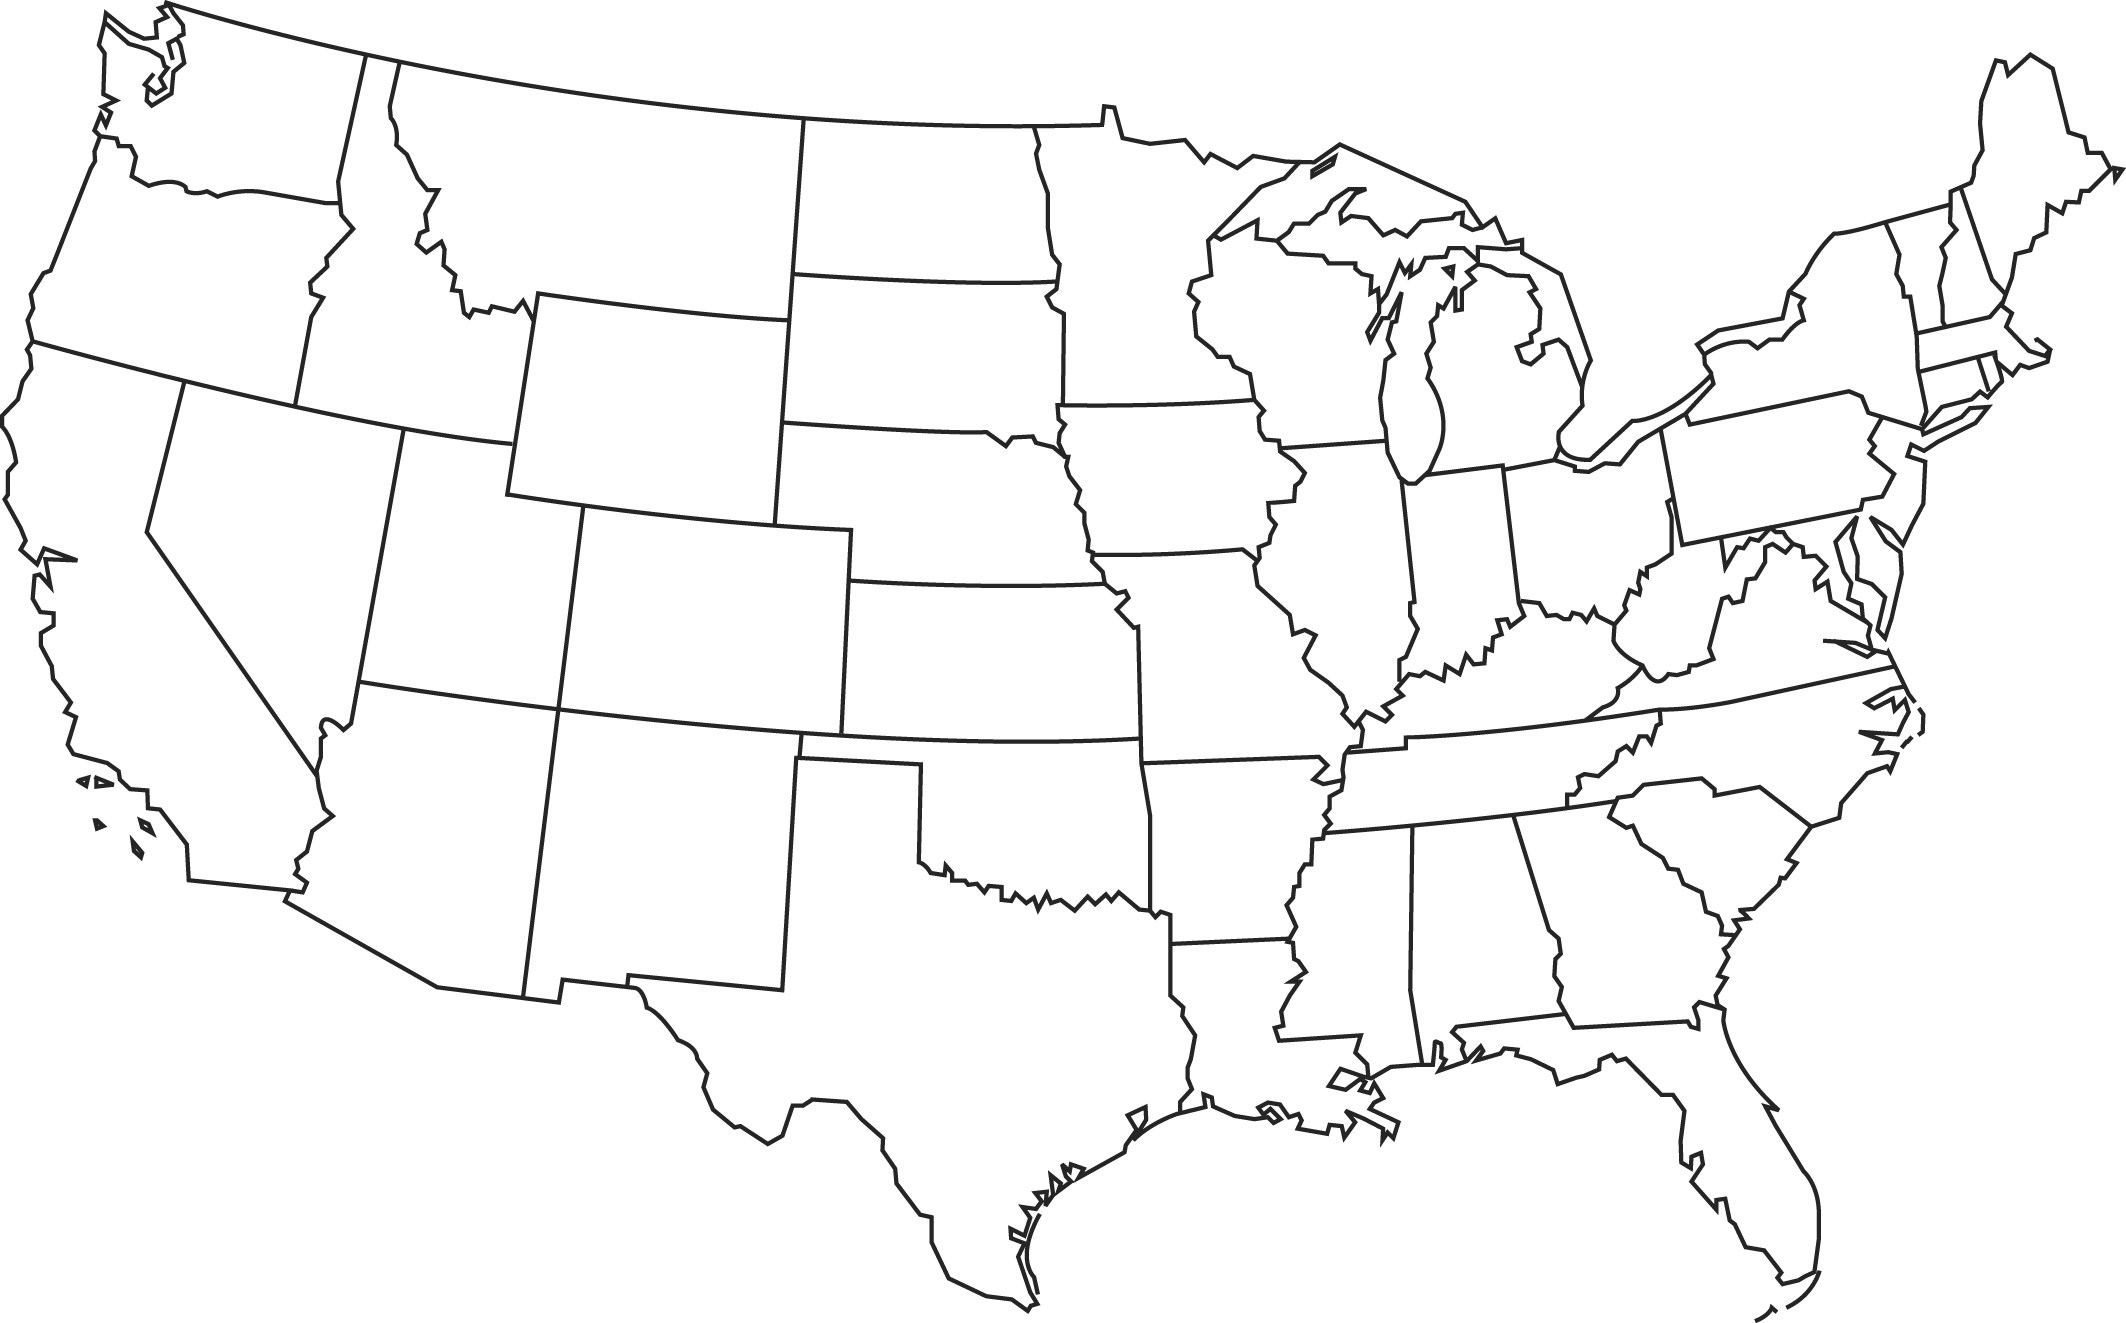
\includegraphics[width=\linewidth]{./images/usa.jpg}
\end{image}%
\tcblower
\end{figureptx}%
\end{exploration}%
\footnotetext[1]{\nolinkurl{./usa_map.pdf}\label{g:fn:idp105544718296976}}%
\begin{theorem}{Four Color Theorem.}{}{g:theorem:idp105544718298768}%
Four colors suffice to color any map such that any two countries which share a part of a border are given different colors.%
\end{theorem}
The proof was very controversial, as it involves the use of computers to check thousands of cases. The proof is generally accepted now, however.%
\par
We can use graphs to model maps. Here is the graph that corresponds to the following map.%
\begin{figureptx}{}{g:figure:idp105544718300048}{}%
\begin{image}{0.25}{0.5}{0.25}%
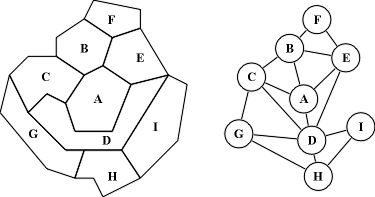
\includegraphics[width=\linewidth]{./images/map1.jpg}
\end{image}%
\tcblower
\end{figureptx}%
\begin{question}{}{g:question:idp105544718300560}%
Why must the graph associated to a map be planar? Why must it have no loops or multiple edges?%
\end{question}
We can't prove the Four Color Theorem, but we can prove that six colors suffice.%
\begin{theorem}{The Six Color Theorem.}{}{g:theorem:idp105544718301456}%
Six colors suffice to color any map such that any two countries which share a part of a border are given different colors.%
\end{theorem}
To do this, we need a definition.%
\begin{definition}{}{g:definition:idp105544718302480}%
Let \(G\) be a graph. The \terminology{degree} of a vertex \(v\) in \(G\) is the number of edges incident to \(v\).%
\end{definition}
\begin{activity}{}{g:activity:idp105544718304912}%
Suppose \(G\) is a graph with \(n\) vertices and that the vertex \(v_i\) has degree \(d_i\). Explain why the following is true:%
\begin{equation*}
d_1 + d_2 + \cdots + d_n = 2\times (\text{the number of edges})
\end{equation*}
(It may help to draw some examples!)%
\end{activity}%
\begin{proposition}{}{}{x:proposition:prop-planar-degree}%
Suppose \(G\) is a planar graph with \(n\) vertices, \(e\) edges, and has no loops or multiple edges between the same pair of vertices. Then%
\begin{equation*}
e \le 3n - 6.
\end{equation*}
%
\end{proposition}
We'll avoid proving this for now, but take it as true. (And it is!)%
\par
As a step on the way to proving the Six Color Theorem, consider the following exploration.%
\begin{exploration}{}{g:exploration:idp105544718277520}%
In this activity, we'll seek to understand the following claim: \begin{quote}%
Every planar graph \(G\) with no loops or multiple edges must contain at least one vertex of degree less than or equal to 5.\end{quote}
 We'll approach this by assuming the conclusion is false and reaching a contradiction.%
%
\begin{itemize}[label=\textbullet]
\item{}To assume the conclusion is false, we should assume that each vertex of \(G\) has degree at least what?%
\item{}Let \(v\) denote the number of vertices in the graph. Since every edge has two ends, the number of edges \(e\) in the graph is \(e =6v/2 = 3v\). Why is this a problem?%
\item{}What if there are vertices of degree larger than 6?%
\item{}Why can we conclude that every planar graph with no loops or multiple edges must have a vertex of degree 5 or less?%
\end{itemize}
\end{exploration}%
We now explore the idea behind the proof of the Six Color Theorem.%
\begin{exploration}{}{g:exploration:idp105544718282256}%
Let \(G\) be a planar graph with \(v\) vertices and \(e\) edges, and no loops or multiple edges.%
%
\begin{enumerate}
\item{}If \(v \le 6\), why are we done?%
\item{}Now consider a graph with \(v = 7\). Why must we have a vertex \(v_0\) of degree 5 or less?%
\item{}Temporarily remove \(v_0\) and any associated edges. How many colors are required for what remains? How many of those colors were used on the neighbors of \(v_0\)?%
\item{}Explain why there is a 6-coloring of \(G\) with \(v_0\) added back in.%
\item{}What if our graph has 8 vertices?%
\item{}What if our graph has 9? Or \(n\), for any \(n\ge 1\)?%
\end{enumerate}
\end{exploration}%
Lest you think graph coloring is just a fun game, consider the following version of a very real situation.%
\begin{activity}{}{g:activity:idp105544718289680}%
Suppose your friendly local university is looking to schedule its final exams. Obviously, it can't schedule them so that someone in two different classes is scheduled for an exam at the same time. But how many times are actually required?%
%
\begin{enumerate}
\item{}First, make up a list of at least 5 courses, and 10 students who are in some of these courses. Ensure that each course shares at least one student in common with at least two other courses (this is just to make the problem sufficiently interesting).%
\item{}Create a graph whose vertices are the courses. Draw an edge between any pair of courses for which a student is enrolled in both courses.%
\item{}How many colors are required to color the vertices so that no pair of adjacent vertices gets the same color? \emph{Can} the answer be more than 4? Why or why not?%
\item{}How many final exam timeslots are required?%
\end{enumerate}
\end{activity}%
\end{sectionptx}
%
%
\typeout{************************************************}
\typeout{Section 5.4 Intro to Trees}
\typeout{************************************************}
%
\begin{sectionptx}{Intro to Trees}{}{Intro to Trees}{}{}{x:section:sec-trees}
Two fundamental questions in the analysis of graphs are: given two vertices, is there a path between them? And if so, how can we find the shortest possible path? Let's consider the second question first.%
\par
Notice in the graph in \hyperref[x:figure:fig-graphexample3]{Figure~{\xreffont\ref{x:figure:fig-graphexample3}}} that there are several paths between, say, \(a\) and \(f\). There is a path spanning two edges: \(a \to c \to f\). There is also a path spanning four edges: \(a\to c \to d \to e \to f\). In general, by the \terminology{distance} between two vertices, we mean a path consisting of the fewest edges possible, so the distance between \(a\) and \(f\) is 1.%
\begin{activity}{}{g:activity:idp105544718329232}%
Consider the graph in \hyperref[x:figure:fig-distance]{Figure~{\xreffont\ref{x:figure:fig-distance}}}.%
\begin{figureptx}{A graph.}{x:figure:fig-distance}{}%
\begin{image}{0.25}{0.5}{0.25}%
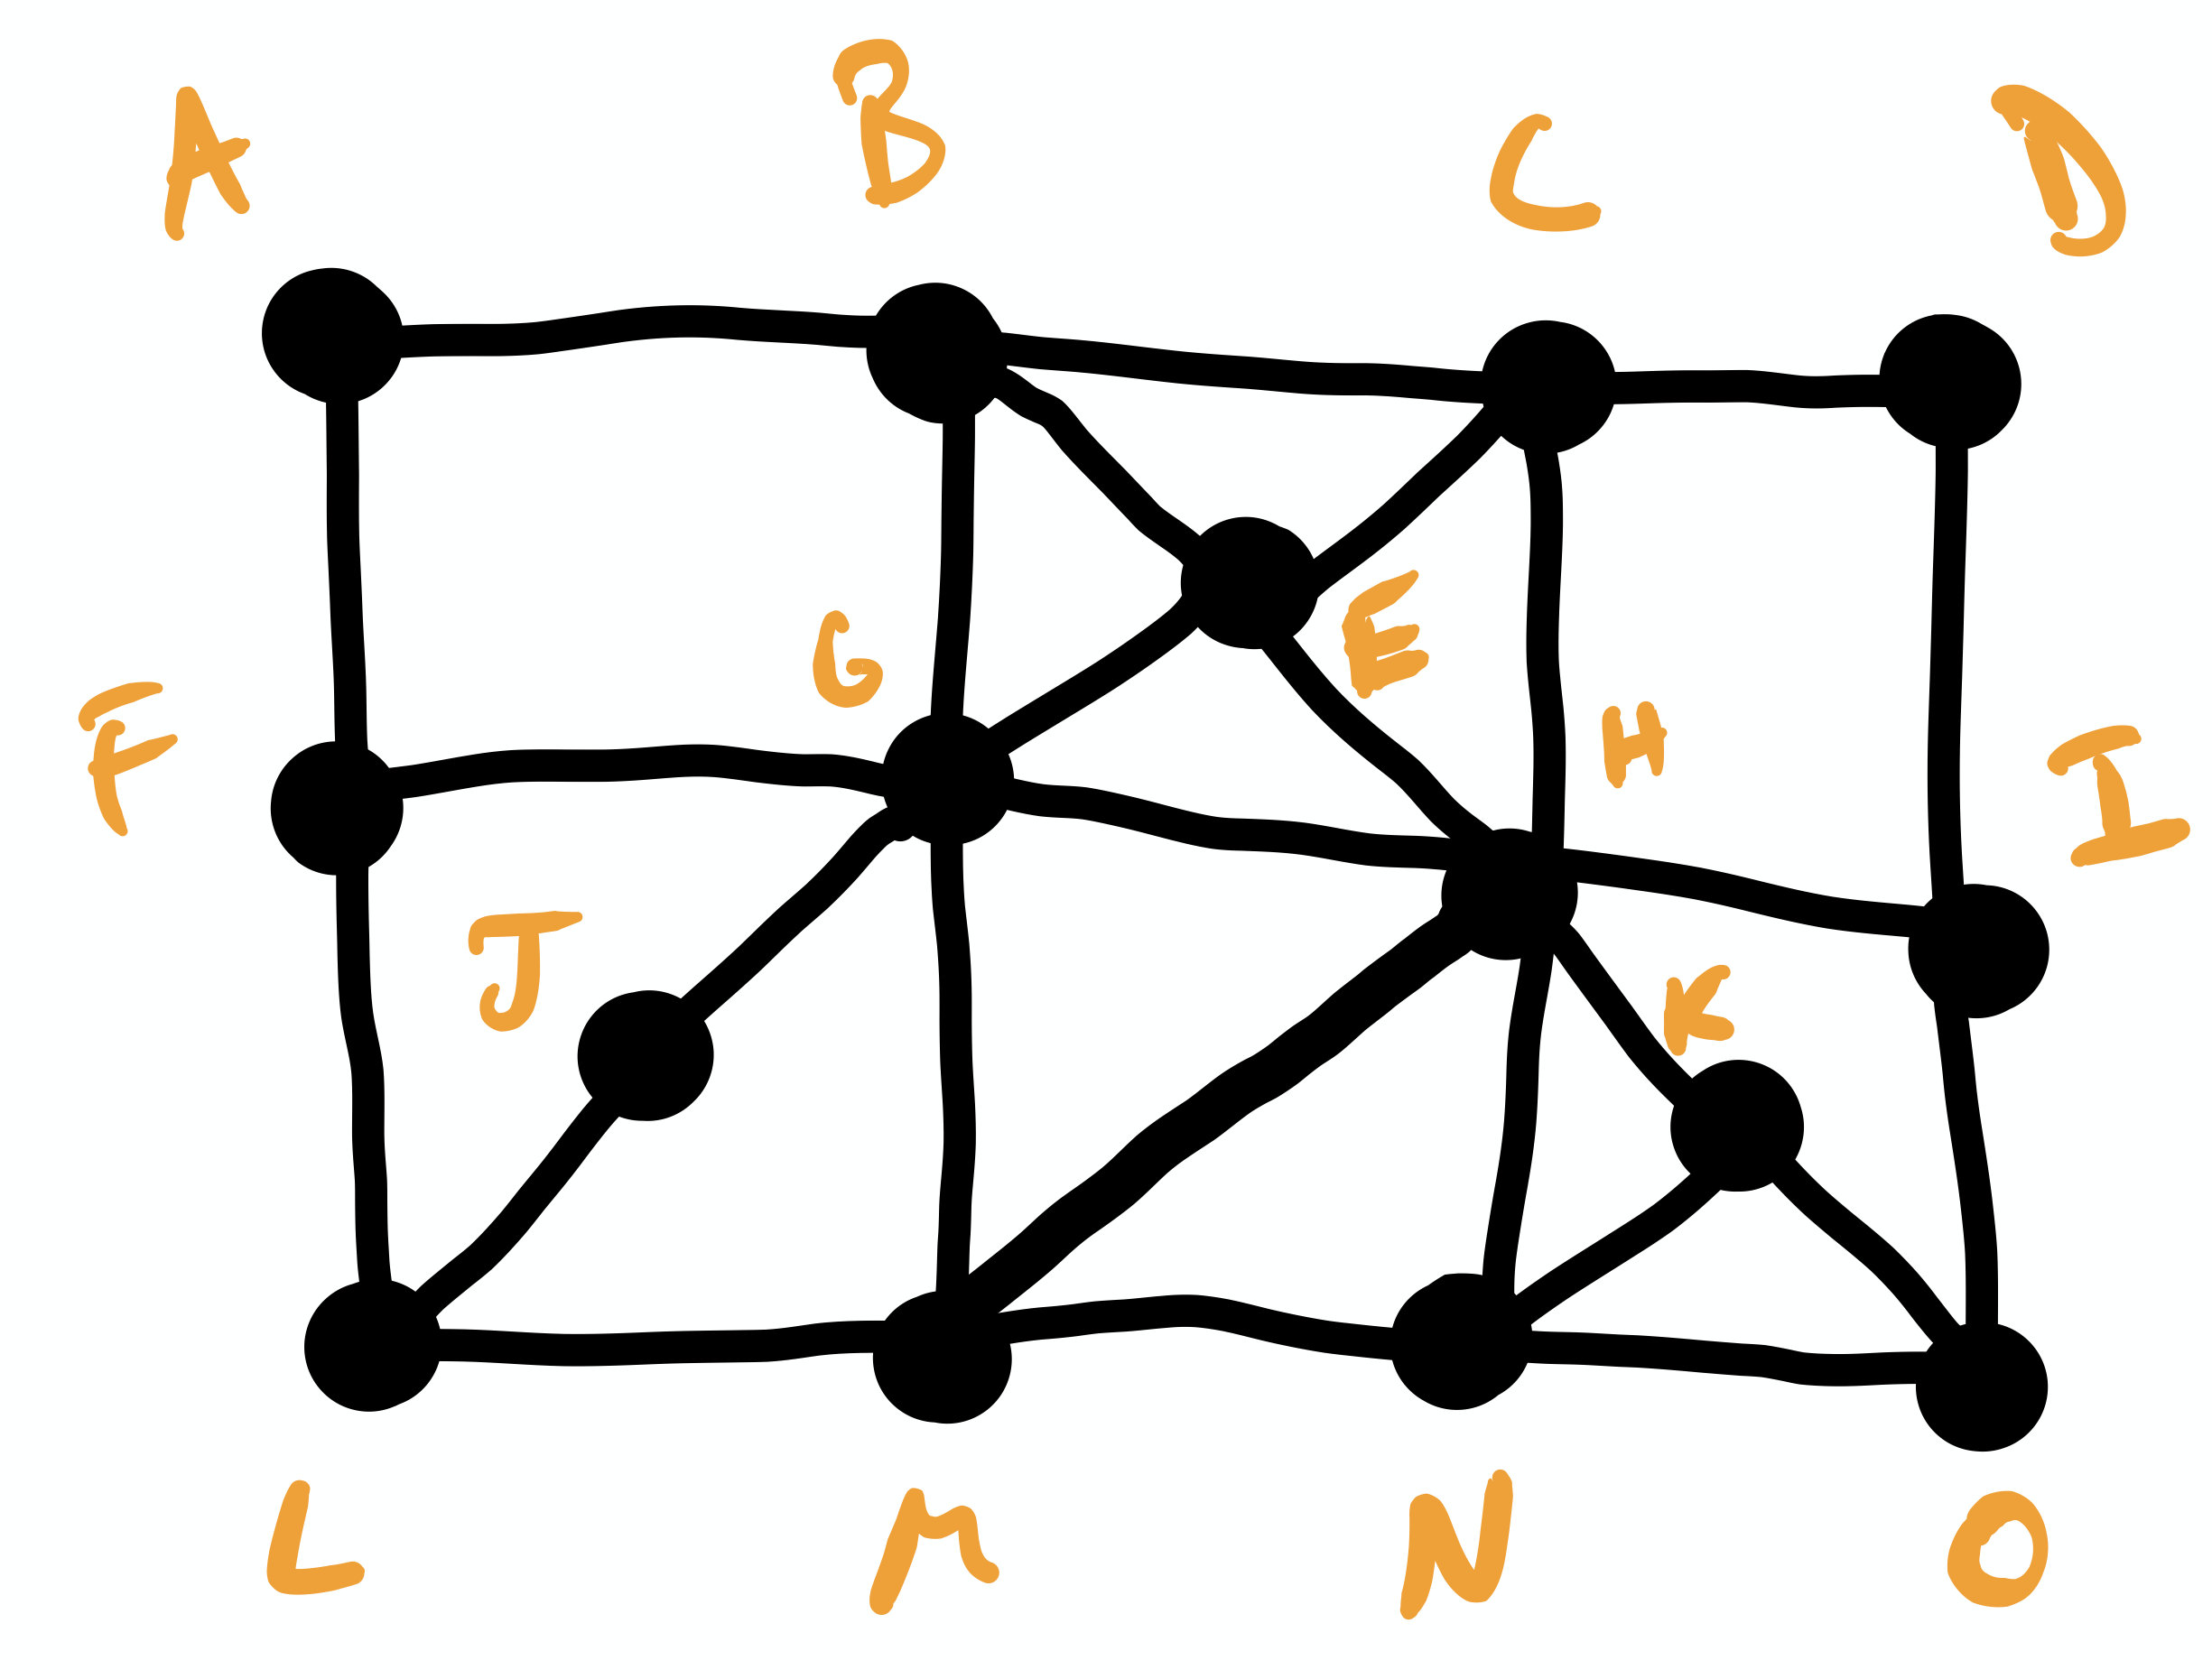
\includegraphics[width=\linewidth]{images/graph04.png}
\end{image}%
\tcblower
\end{figureptx}%
%
\begin{enumerate}
\item{}Find three paths from vertex \(L\) to vertex \(E\).%
\item{}Determine the distance from vertex \(B\) to vertex \(N\). How many paths of this distance can you find?%
\end{enumerate}
\end{activity}%
Returning to the first question above, if the graph is connected, the answer is obviously \emph{yes}. So, given a graph \(G(V,E)\), we are often interested in removing superfluous edges in a systematic way to arrive at a smallest (which will be made precise shortly) connected \terminology{subgraph} \(T(V,E')\).%
\begin{definition}{}{g:definition:idp105544718335376}%
A \terminology{cycle} on \(n\) vertices \(v_1, v_2, \ldots, v_n\) is the graph with \(n+1\) edges \(v_1 v_2, v_2 v_3, \ldots, v_{n-1} v_n, v_n v_1\). We denote such a cycle by \(C_n\). That is, a cycle consists of a path \(v_1 \to v_2 \to v_3 \to \ldots \to v_n \to v_1\), where the only repeated vertex is the first\slash{}last one.%
\end{definition}
\begin{example}{}{g:example:idp105544718338448}%
\setlength{\qrsize}{9em}
\setlength{\previewwidth}{\linewidth}
\addtolength{\previewwidth}{-\qrsize}
\begin{tcbraster}[raster columns=2, raster column skip=1pt, raster halign=center, raster force size=false, raster left skip=0pt, raster right skip=0pt]%
\begin{tcolorbox}[previewstyle, width=\previewwidth]%
\includegraphics[width=0.80\linewidth,height=\qrsize,keepaspectratio]{images/video-1.jpg}%
\end{tcolorbox}%
\begin{tcolorbox}[qrstyle]%
{\hypersetup{urlcolor=black}\qrcode[height=\qrsize]{https://www.youtube.com/watch?v=iu-Zm4xBYw4}}%
\end{tcolorbox}%
\begin{tcolorbox}[captionstyle]%
\small YouTube: \mono{https://www.youtube.com/watch?v=iu-Zm4xBYw4}\end{tcolorbox}%
\end{tcbraster}%
\end{example}
One of the major questions in theoretical graph theory is: given a graph \(G\), is there an algorithm that determines whether \(G\) contains any cycles? There are several such algorithms, and they are relatively efficient. A related question is: given a graph \(G\), is there an efficient algorithm which can produce a cycle that visits each vertex exactly once? The answer to this question is currently unknown (as of April 2020), but an active area of research. \begin{aside}{}{g:aside:idp105544718340240}%
\end{aside}
%
\par
Our focus for the rest of this section is graphs that do \emph{not} contain any cycles.%
\begin{definition}{}{x:definition:def-tree}%
\index{tree}%
A connected graph \(T(V,E)\) that does not contain any cycles is known as a \terminology{tree}. \begin{aside}{}{g:aside:idp105544718310416}%
\end{aside}
%
\end{definition}
\begin{example}{}{g:example:idp105544718311568}%
\setlength{\qrsize}{9em}
\setlength{\previewwidth}{\linewidth}
\addtolength{\previewwidth}{-\qrsize}
\begin{tcbraster}[raster columns=2, raster column skip=1pt, raster halign=center, raster force size=false, raster left skip=0pt, raster right skip=0pt]%
\begin{tcolorbox}[previewstyle, width=\previewwidth]%
\includegraphics[width=0.80\linewidth,height=\qrsize,keepaspectratio]{images/video-2.jpg}%
\end{tcolorbox}%
\begin{tcolorbox}[qrstyle]%
{\hypersetup{urlcolor=black}\qrcode[height=\qrsize]{https://www.youtube.com/watch?v=2Qy8fugua80}}%
\end{tcolorbox}%
\begin{tcolorbox}[captionstyle]%
\small YouTube: \mono{https://www.youtube.com/watch?v=2Qy8fugua80}\end{tcolorbox}%
\end{tcbraster}%
\end{example}
The description given in \hyperref[x:definition:def-tree]{Definition~{\xreffont\ref{x:definition:def-tree}}} is pretty close to what we want. Given a graph \(G(V,E)\), we want a tree \(T(V,E')\) such that every vertex of \(G\) is also a vertex of \(T\), and every edge of \(T\) to be an edge of \(G\). Such a tree is known as a \terminology{spanning tree} for \(G\).%
\begin{exploration}{}{g:exploration:idp105544718315664}%
Determine whether the given graph is a tree. Justify your answer by making explicit reference to \hyperref[x:definition:def-tree]{Definition~{\xreffont\ref{x:definition:def-tree}}}.%
%
\begin{enumerate}
\item{}\begin{figureptx}{The graph for Question 1. Is it a tree, or no?}{x:figure:fig-treeq01}{}%
\begin{image}{0.25}{0.5}{0.25}%
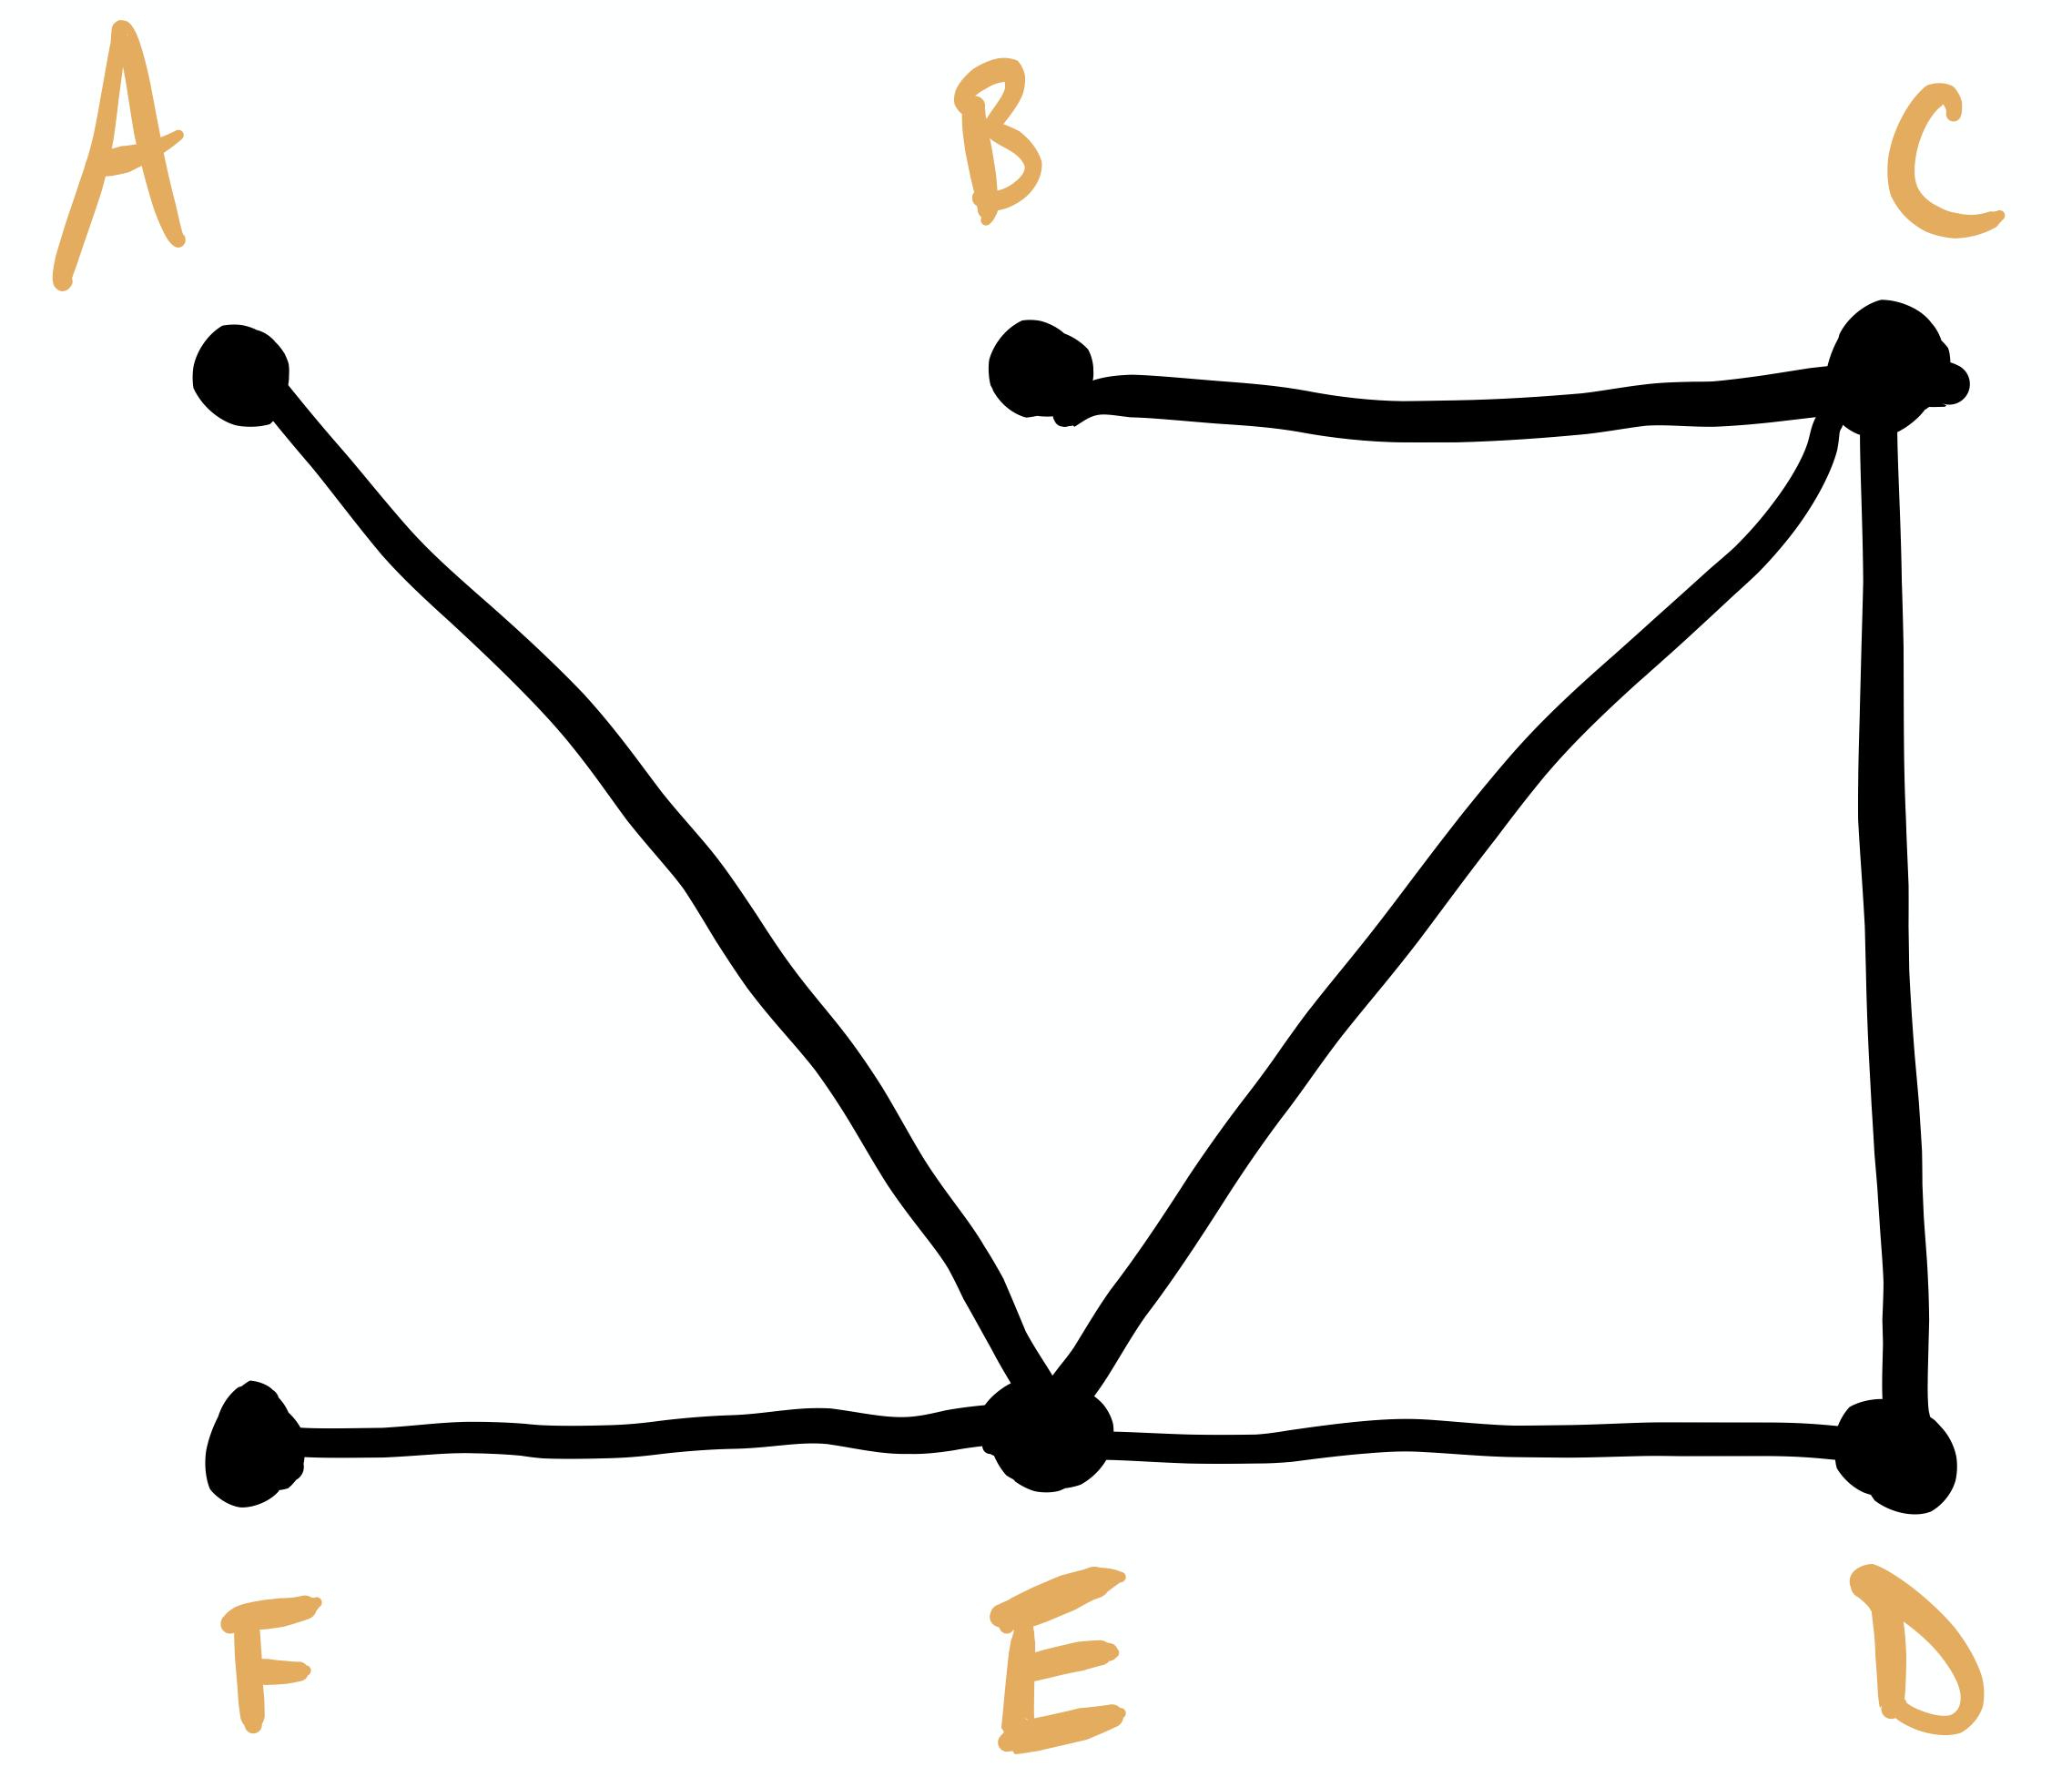
\includegraphics[width=\linewidth]{images/tree01.png}
\end{image}%
\tcblower
\end{figureptx}%
%
\item{}\begin{figureptx}{The graph for Question 2. Is it a tree, or no?}{x:figure:fig-treeq02}{}%
\begin{image}{0.25}{0.5}{0.25}%
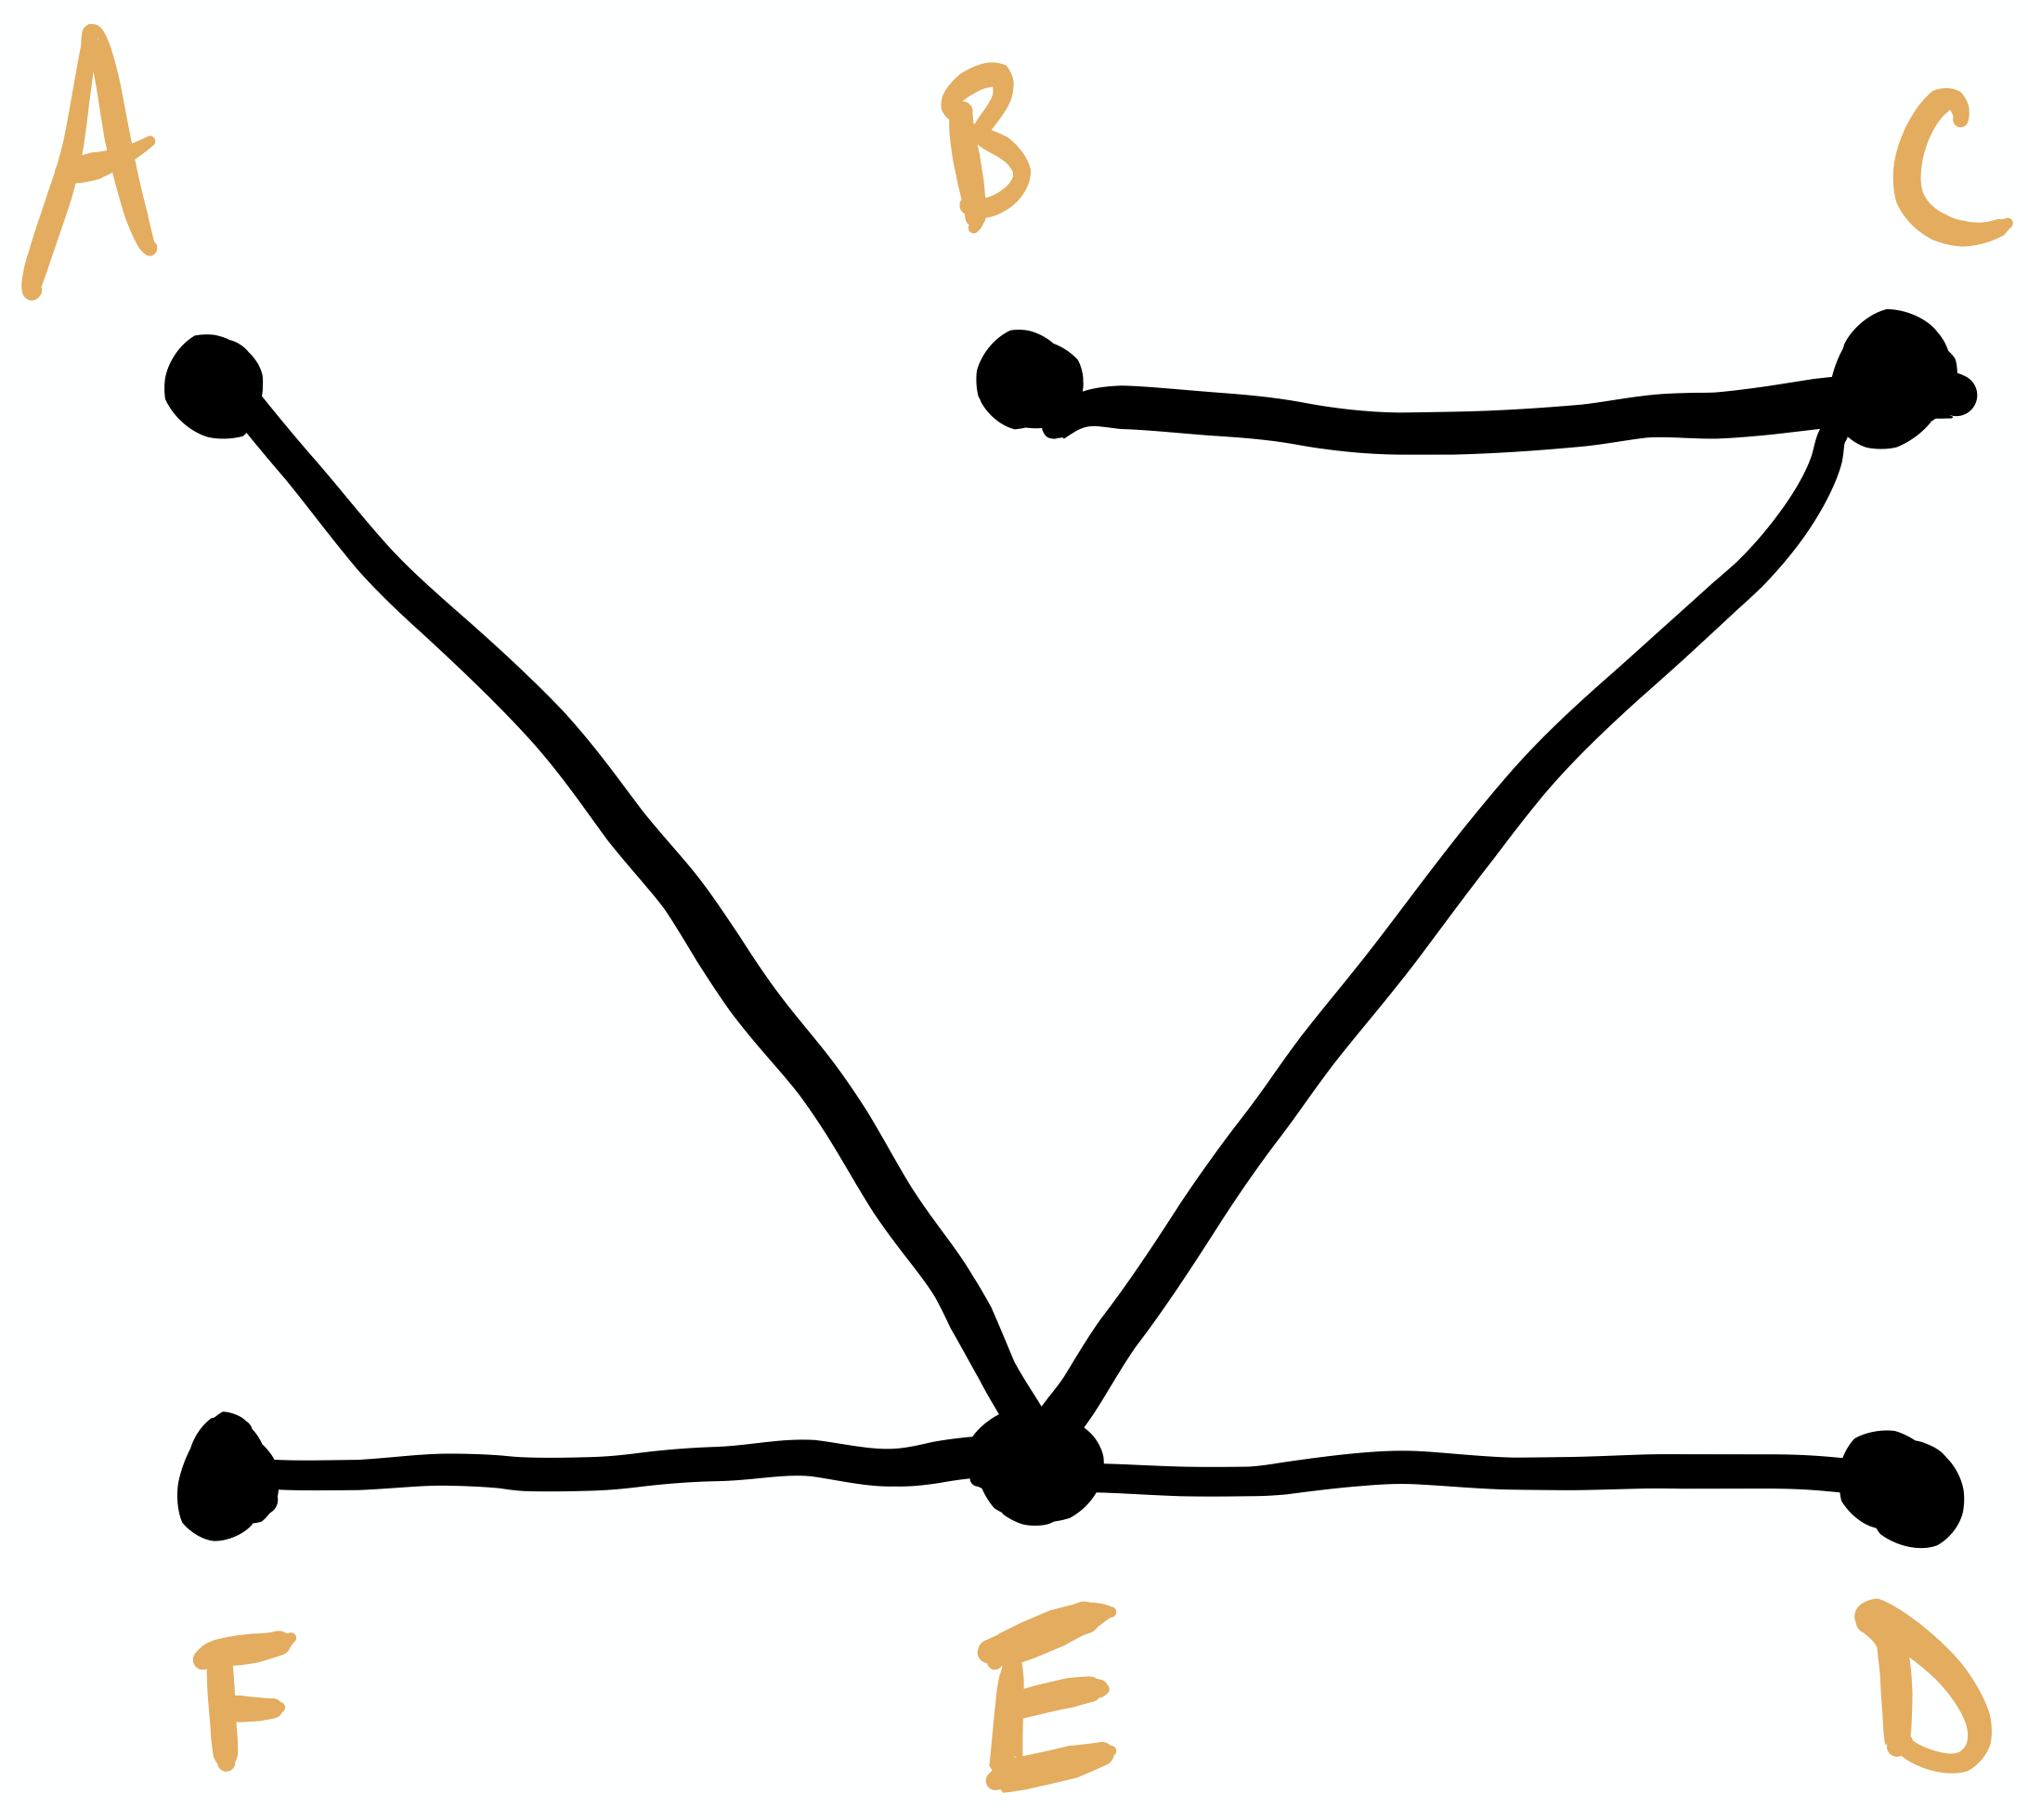
\includegraphics[width=\linewidth]{images/tree02.png}
\end{image}%
\tcblower
\end{figureptx}%
%
\item{}\begin{figureptx}{The graph for Question 3. Is it a tree, or no?}{x:figure:fig-treeq03}{}%
\begin{image}{0.25}{0.5}{0.25}%
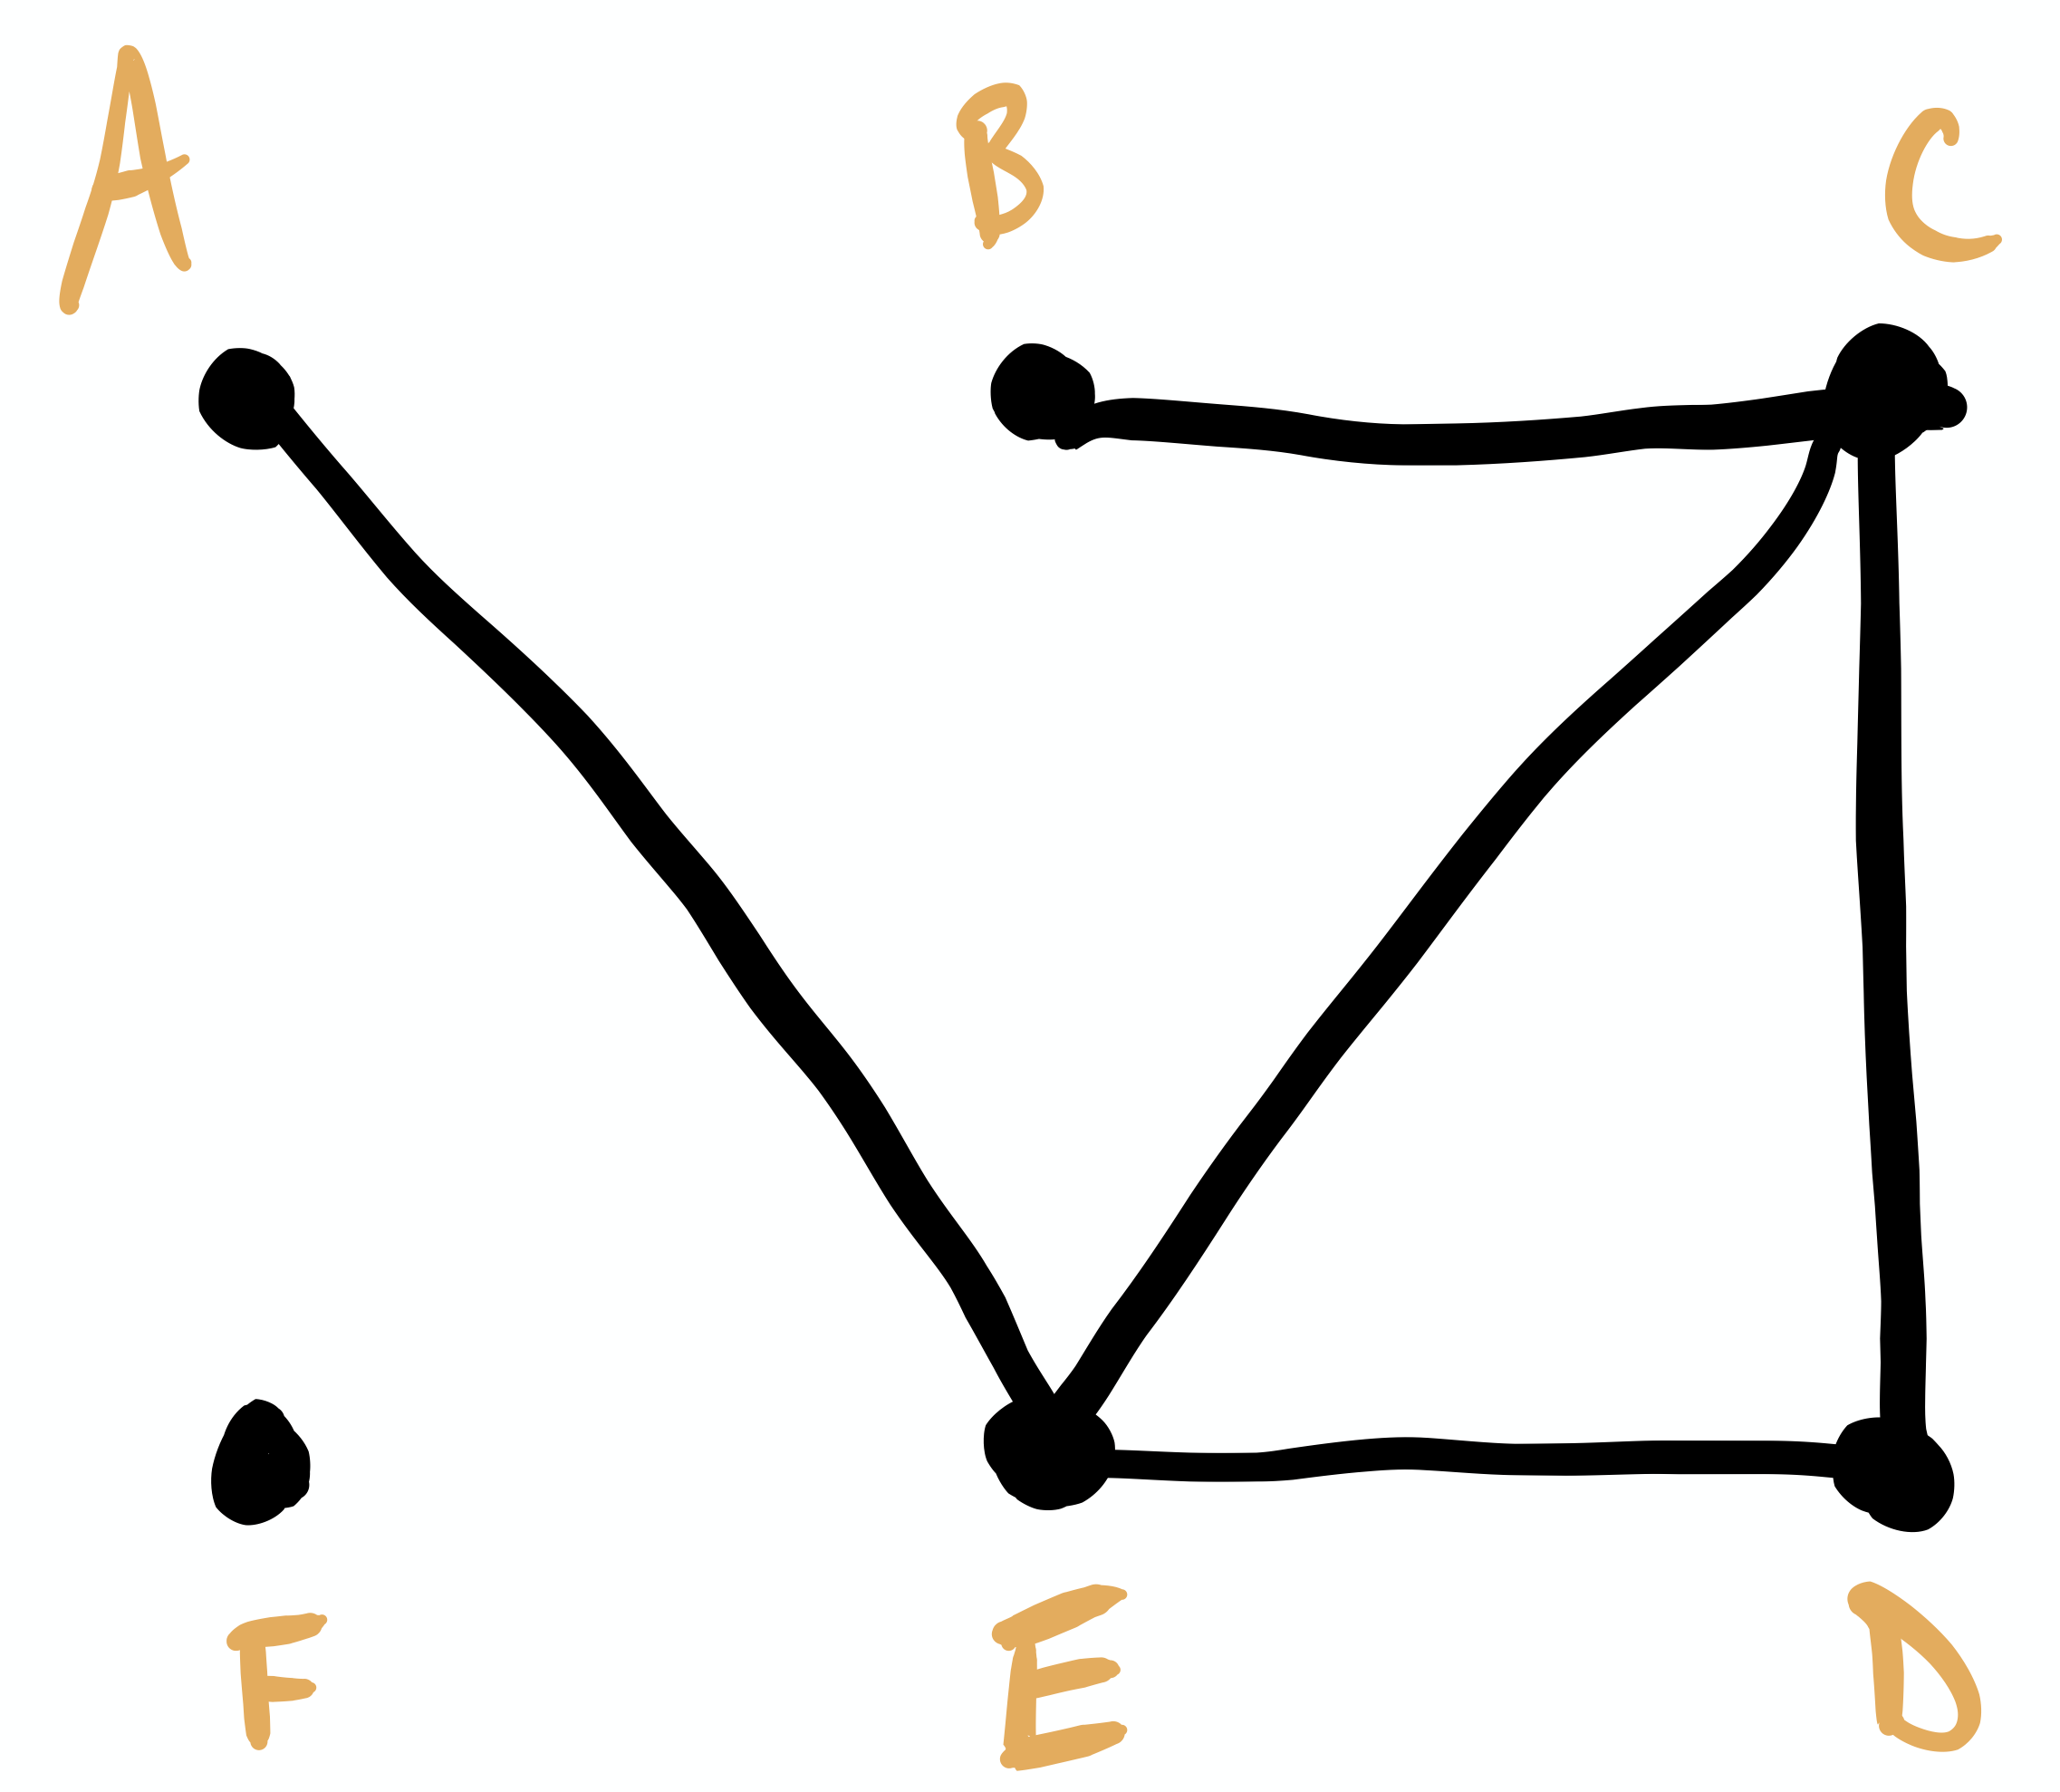
\includegraphics[width=\linewidth]{images/tree03.png}
\end{image}%
\tcblower
\end{figureptx}%
%
\end{enumerate}
\end{exploration}%
The last big idea that we'll explore is the notion of a \(weighted\) graph, which we introduce with an example.%
\begin{example}{}{g:example:idp105544718321808}%
Consider the graph in \hyperref[x:figure:fig-conveyorbelt]{Figure~{\xreffont\ref{x:figure:fig-conveyorbelt}}}. Suppose the vertices represent stations in a factory, and the edges represent conveyor belts between the stations.%
\begin{figureptx}{A graph representing the arrangements of conveyor belts between four stations in a factory.}{x:figure:fig-conveyorbelt}{}%
\begin{image}{0.25}{0.5}{0.25}%
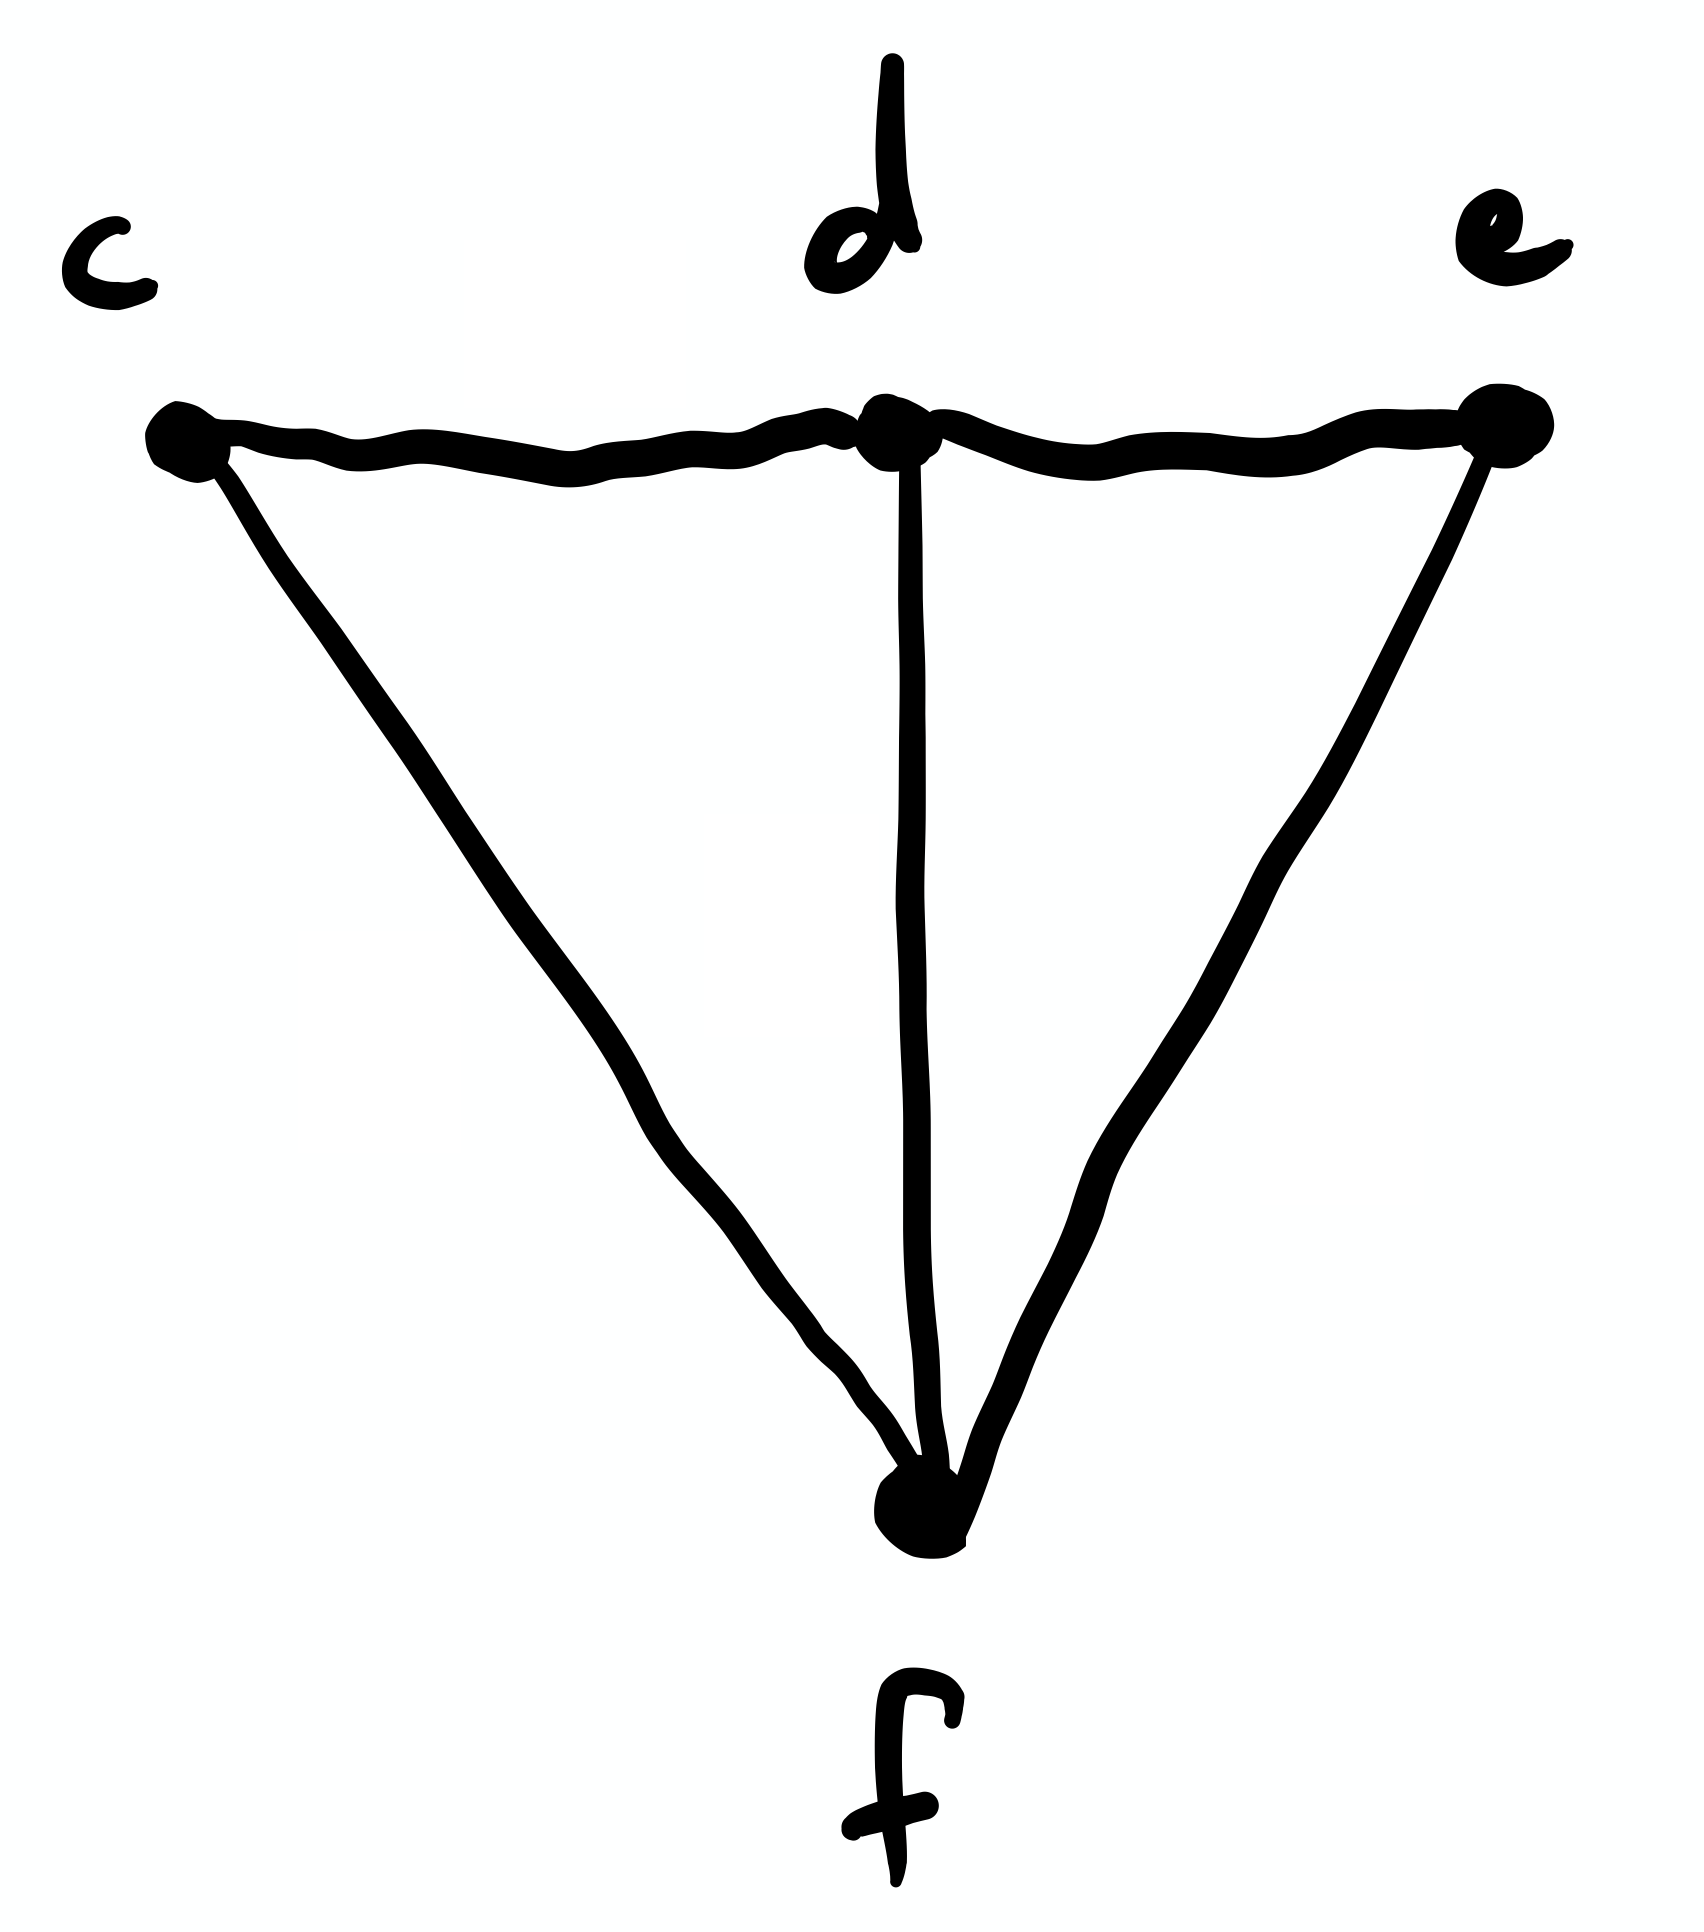
\includegraphics[width=\linewidth]{images/graph06.png}
\end{image}%
\tcblower
\end{figureptx}%
A manager in the factory may be interested in how efficiently the conveyor belts can be run. Suppose that belt \(cd\) costs \textdollar{}11\slash{}day to run, belt \(de\) costs \textdollar{}8\slash{}day to run, belt \(cf\) costs \textdollar{}9\slash{}day to run, belt \(df\) costs \textdollar{}12\slash{}day to run, and belt \(ef\) costs \textdollar{}11\slash{}day to run. We can represent this by labeling each edge with its cost, as seen in \hyperref[x:figure:fig-weightedbelt]{Figure~{\xreffont\ref{x:figure:fig-weightedbelt}}}.%
\begin{figureptx}{A \emph{weighted} graph representing the arrangements of conveyor belts between four stations in a factory.}{x:figure:fig-weightedbelt}{}%
\begin{image}{0.25}{0.5}{0.25}%
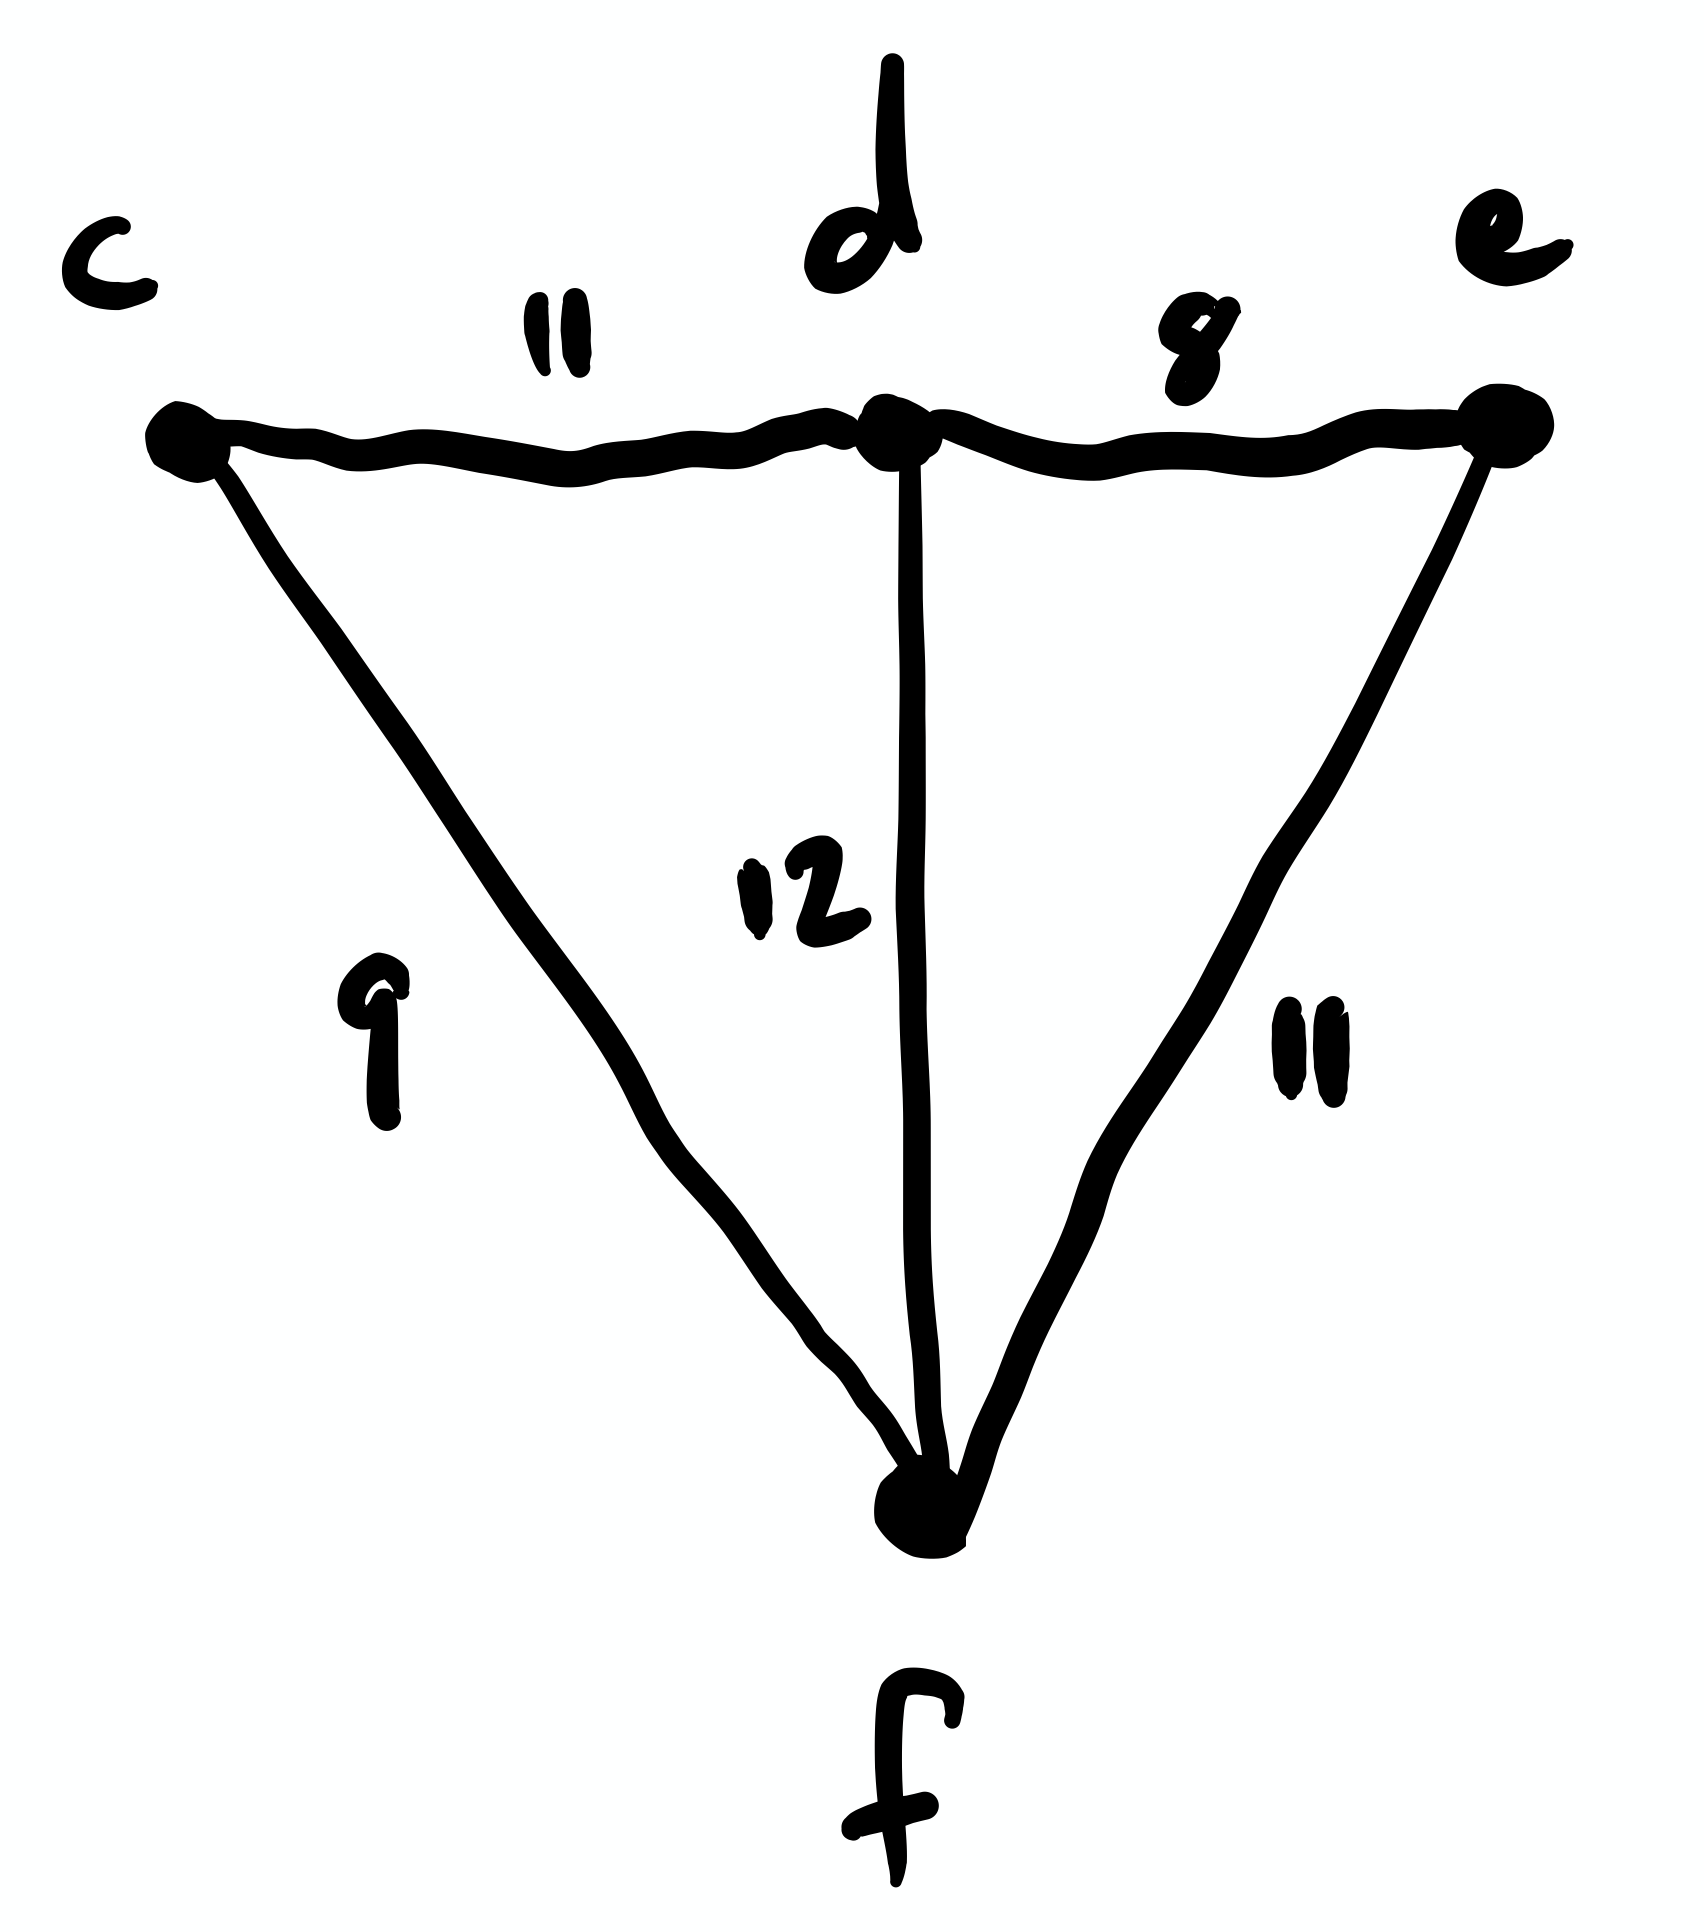
\includegraphics[width=\linewidth]{images/graph05.png}
\end{image}%
\tcblower
\end{figureptx}%
This is an example of a \terminology{weighted graph}, which is just a graph with the edges labeled. The labels usually represent something meaningful about the situation the graph represents. For example, we could have weighted the edges in \hyperref[x:figure:fig-weightedbelt]{Figure~{\xreffont\ref{x:figure:fig-weightedbelt}}} with the time it takes to move an object from one station to another, or the distance between stations (as one might find on a map), etc.%
\end{example}
We tie this all together with the concept of a \terminology{minimal spanning tree}, which is a spanning tree with the smallest total weight.%
\begin{example}{}{x:example:ex-mwst-elimination}%
Again, consider the weighted graph representing our conveyor belt in \hyperref[x:figure:fig-weightedbelt]{Figure~{\xreffont\ref{x:figure:fig-weightedbelt}}}. The total cost to run the belts for one day is \textdollar{}51. Assume that eliminating a belt does not substantially increase the cost of running the others. How could we find a lower-cost arrangement?%
\setlength{\qrsize}{9em}
\setlength{\previewwidth}{\linewidth}
\addtolength{\previewwidth}{-\qrsize}
\begin{tcbraster}[raster columns=2, raster column skip=1pt, raster halign=center, raster force size=false, raster left skip=0pt, raster right skip=0pt]%
\begin{tcolorbox}[previewstyle, width=\previewwidth]%
\includegraphics[width=0.80\linewidth,height=\qrsize,keepaspectratio]{images/video-3.jpg}%
\end{tcolorbox}%
\begin{tcolorbox}[qrstyle]%
{\hypersetup{urlcolor=black}\qrcode[height=\qrsize]{https://www.youtube.com/watch?v=fXfsHOVSy2U}}%
\end{tcolorbox}%
\begin{tcolorbox}[captionstyle]%
\small YouTube: \mono{https://www.youtube.com/watch?v=fXfsHOVSy2U}\end{tcolorbox}%
\end{tcbraster}%
\end{example}
There are several algorithms for finding minimum weight spanning trees in addition to the one presented in \hyperref[x:example:ex-mwst-elimination]{Example~{\xreffont\ref{x:example:ex-mwst-elimination}}}. A famous such example is \terminology{Prim's algorithm}.%
\begin{algorithm}{Prim's Algorithm.}{}{x:algorithm:alg-prim}%
\setlength{\qrsize}{9em}
\setlength{\previewwidth}{\linewidth}
\addtolength{\previewwidth}{-\qrsize}
\begin{tcbraster}[raster columns=2, raster column skip=1pt, raster halign=center, raster force size=false, raster left skip=0pt, raster right skip=0pt]%
\begin{tcolorbox}[previewstyle, width=\previewwidth]%
\includegraphics[width=0.80\linewidth,height=\qrsize,keepaspectratio]{images/video-4.jpg}%
\end{tcolorbox}%
\begin{tcolorbox}[qrstyle]%
{\hypersetup{urlcolor=black}\qrcode[height=\qrsize]{https://www.youtube.com/watch?v=QoF1b9t4DGQ}}%
\end{tcolorbox}%
\begin{tcolorbox}[captionstyle]%
\small YouTube: \mono{https://www.youtube.com/watch?v=QoF1b9t4DGQ}\end{tcolorbox}%
\end{tcbraster}%
\end{algorithm}
\end{sectionptx}
\end{chapterptx}
 %
%
\typeout{************************************************}
\typeout{Chapter 6 Modular Arithmetic and Coding Theory}
\typeout{************************************************}
%
\begin{chapterptx}{Modular Arithmetic and Coding Theory}{}{Modular Arithmetic and Coding Theory}{}{}{x:chapter:chap-coding}
%
%
\typeout{************************************************}
\typeout{Section 6.1 Adding in Circles}
\typeout{************************************************}
%
\begin{sectionptx}{Adding in Circles}{}{Adding in Circles}{}{}{x:section:sec-intro-to-mod-arithmetic}
\begin{assemblage}{Motivating Questions.}{g:assemblage:idp105544716531984}%
In this section, we will explore the following questions. %
\begin{enumerate}
\item{}What is congruence modulo \(m\)?%
\item{}What are some real-world examples of congruence?%
\item{}How can we do arithemtic modulo \(m\)?%
\end{enumerate}
%
\end{assemblage}
This topic comes to us from the realm of mathematics known as \emph{number theory}, which is all about the properties of the integers: positive whole numbers, negatives of whole numbers, and zero. Number theory is one of the oldest branches of mathematics; some of its hallmark theorems, still vital and taught today, have been known for thousands of years. And many of the deep structural features of the integers have found modern application in the hiding and transmitting of information. It is toward this last application that we now turn.%
\par
First, however, we need to be reminded of a suprisingly important result from school mathematics. We begin with some warmup questions.%
\begin{hypothesis}{}{}{x:hypothesis:warmup-long-division}%
For each pair of positive integers given below, perform long division to divide the first number by the second.%
%
\begin{enumerate}
\item{}42, 6%
\item{}42, 8%
\item{}71, 9%
\item{}0, 17%
\item{}9, 71%
\item{}8675309, 627%
\end{enumerate}
\end{hypothesis}
\begin{assemblage}{The Division Algorithm.}{x:assemblage:thm-divalg}%
Let \(a\) and \(m\) be integers, with \(m\gt 0\). Then there exist unique integers \(q,r\), \(0\le r \lt m\), such that%
\begin{equation*}
a = m\cdot q + r.
\end{equation*}
We call \(a\) the \terminology{dividend}, \(m\) the \terminology{divisor}, \(q\) the \terminology{quotient}, and \(r\) the \terminology{remainder}.%
\end{assemblage}
\begin{activity}{}{g:activity:idp105544716512912}%
For each long division problem from \hyperref[x:hypothesis:warmup-long-division]{Warmup~{\xreffont\ref{x:hypothesis:warmup-long-division}}}, identify the dividend, divisor, quotient, and remainder as described in \hyperref[x:assemblage:thm-divalg]{the Division Algorithm}. What do you notice? What do you wonder?%
\end{activity}%
\begin{principle}{}{}{g:principle:idp105544716514704}%
What is meant by the word ``unique'' in \hyperref[x:assemblage:thm-divalg]{the Division Algorithm}? Or, put slightly differently, when dividing 71 by 9, why do you think we do we not give a quotient of 6 and remainder of 17?%
\end{principle}
Of primary importance for us will be a consideration of the remainders obtained by dividing by a fixed positive integer \(m\gt 1\).%
\begin{activity}{}{x:activity:act-remainders}%
Throughout this activity, we will be dividing by \(m = 5\). However, you should be thinking about how the answers might differ if we divide by a different integer \(m\).%
%
\begin{enumerate}
\item{}What remainders do you obtain when dividing the integers \(12, 16, 20, 24, 33\) by 5?%
\item{}What remainders do you obtain when dividing the integers \(39, 52, 80, 108, 166\) by 5?%
\item{}What remainders are \emph{possible} upon division by 5? How do you know?%
\item{}What remainders do you expect to be possible upon division by 103? How do you know?%
\item{}For each of the five integers from the first question, find the integer from the second question whose remainder upon division by 5 is the same and write the pairs in a list.%
\item{}For each pair in the list you made in the previous question, find the difference between the two integers and divide \emph{that number} by \(m=5\). What do you notice? What do you wonder?%
\end{enumerate}
\end{activity}%
The work you did in \hyperref[x:activity:act-remainders]{Activity~{\xreffont\ref{x:activity:act-remainders}}} provides motivation for the following definition.%
\begin{definition}{}{x:definition:def-congruence}%
\index{congruence modulo \(m\)}%
\index{modulus}%
Let \(a,b\) be integers and \(m \gt 1\) an integer. We say that \(a\) and \(b\) are \terminology{congruent modulo \(m\)} if \(a\) and \(b\) have the same remainder upon division by \(m\). In this case, we write \(a\equiv b\mod m\) and call \(m\) the \terminology{modulus}.%
\par
Equivalently, we say \(a\) and \(b\) are congruent modulo \(m\) if \(m\) evenly divides \(b-a\).%
\end{definition}
Let's explore this definition a bit more.%
\begin{activity}{}{g:activity:idp105544716564240}%
For the given values below, determine whether \(a \equiv b\mod m\).%
%
\begin{enumerate}
\item{}\(a = 71\), \(b = 39\), \(m= 16\)%
\item{}\(a = 17\), \(b = 19\), \(m = 4\)%
\item{}\(a = 832\), \(b = 584\), \(m= 31\)%
\end{enumerate}
\end{activity}%
Congruence modulo \(m\) possesses several important properties. We highlight three of them in the following theorem.%
\begin{theorem}{}{}{x:theorem:thm-congruence-equiv-relation}%
Let \(m\gt 1\) be an integer, and suppose \(a,b,c\) are integers.%
%
\begin{itemize}[label=\textbullet]
\item{}Congruence is \terminology{reflexive}: \(a\equiv a\mod m\)%
\item{}Congruence is \terminology{symmetric}: If \(a\equiv b\mod m\), then \(b\equiv a\mod m\).%
\item{}Congruence is \terminology{transitive}: If \(a\equiv b\mod m\) and \(b\equiv c\mod m\), then \(a\equiv c\mod m\).%
\end{itemize}
\end{theorem}
Now that we are a bit more familiar with the definition, let's test its limits.%
\begin{exploration}{}{x:exploration:expl-arithmetic-mod-m}%
Choose two different values of \(m\), and for each value you choose, find two values of \(a\) and \(b\) so that \(a\equiv b\mod m\).%
%
\begin{enumerate}
\item{}Now choose a third integer \(c\). For the integers you chose, is it true that \(a+c \equiv b+c\mod m\)? Is it true that \(a-c \equiv b-c\mod m\)? What about \(a\cdot c\equiv b\cdot c\mod m\)?%
\item{}For each integer \(c\) you chose, find an integer \(d\) such that \(c\equiv d\mod m\). Is it true that \(a+c \equiv b+d\mod m\)? Is it true that \(a-c \equiv b-d\mod m\)? What about \(a\cdot c \equiv b\cdot d\mod m\)?%
\item{}Finally, note that \(5\cdot 2 \equiv 3\cdot 2\mod 4\). Does it follow that \(5\equiv 3\mod 4\)?%
\end{enumerate}
\end{exploration}%
Our discoveries in \hyperref[x:exploration:expl-arithmetic-mod-m]{Exploration~{\xreffont\ref{x:exploration:expl-arithmetic-mod-m}}} delineate the operations known as \terminology{modular arithmetic}: we may add, subtract, and multipy integers mod \(m\), but we may not divide.%
\begin{activity}{}{g:activity:idp105544716552080}%
Find the smallest nonnegative integer \(x\) satisfying:%
%
\begin{enumerate}
\item{}\(\displaystyle x\equiv 9\cdot 4\mod 5\)%
\item{}\(\displaystyle x\equiv 103+405\mod 10\)%
\item{}\(\displaystyle x \equiv 56 + 6\mod 7\)%
\item{}\(\displaystyle x \equiv 9\cdot 99\mod 5\)%
\end{enumerate}
\end{activity}%
\begin{assemblage}{Questions.}{g:assemblage:idp105544716554896}%
Consider the following questions, and what they have to do with modular arithmetic. %
\begin{enumerate}
\item{}What day of the week will it be 62 days from now?%
\item{}What month will it be 40 months from now?%
\item{}What time will it be 27 hours from now?%
\end{enumerate}
%
\end{assemblage}
\end{sectionptx}
%
%
\typeout{************************************************}
\typeout{Section 6.2 Coding Theory}
\typeout{************************************************}
%
\begin{sectionptx}{Coding Theory}{}{Coding Theory}{}{}{x:section:sec-coding}
\begin{assemblage}{Motivating Questions.}{g:assemblage:idp105544716590480}%
In this section, we will explore the following questions. %
\begin{enumerate}
\item{}How can modular arithmetic be applied to the transmission of information?%
\item{}How does the UPC check digit scheme work? What errors can it detect? What errors can it correct?%
\end{enumerate}
%
\end{assemblage}
In \hyperref[x:section:sec-intro-to-mod-arithmetic]{Section~{\xreffont\ref{x:section:sec-intro-to-mod-arithmetic}}}, we learned about modular arithmetic, which works by considering the remainders obtained upon division by a fixed number \(m\). In this section, we'll consider a relatively recent application of modular arithmetic to \terminology{coding theory}, which is the mathematical study of transmitting information.%
\par
The basic problem of coding theory is as follows: in order to send information from one entity to another, it needs to be encoded in some form by the \emph{sender} (e.g., written, recorded, etc) and transmitted across a \emph{channel} (e.g., mailed, emailed, uploaded\slash{}downloaded, etc) to the \emph{receiver}. However, as in the classic game of telephone, errors can creep into the process\textemdash{}written messages can be smudged, physical defects or packet loss can corrupt digital messages, and so on, resulting in information that either cannot be read at all, or can be misread. How can we be reasonably sure that common errors can be detected, and, perhaps, corrected?%
\begin{activity}{}{x:activity:warmup-coding}%
Alice wants to send a bit of information to her friend Bob; for simplicity's sake, let's assume she seeks to send a 0 or 1. To improve the chances that the message is received correctly, she decides to send it three times in a row. So, if Alice desires to send Bob a 1, she'll actually send 111; if she desires to send a 0, she'll send 000.%
%
\begin{enumerate}
\item{}As described above, errors can creep into the transmitted messsage; perhaps Alice sends Bob 111 and that is what he receives, but what if he receives 101? Or 100? How should Bob interpet those two (different) messages?%
\item{}What strengths and weaknesses do you see in Alice's system? How could you improve the chances that Bob interprets Alice's message as she intends?%
\item{}Perhaps you decided that Alice's system is still too prone to errors, so you decide she should send the intended digit seven times instead of 3. In what way(s) is this revised system better? Worse?%
\end{enumerate}
\end{activity}%
Lots of information is encoded using numbers, which makes the reliable transmission of numbers an important problem to solve. A fundamental example is alluded to in \hyperref[x:activity:warmup-coding]{Activity~{\xreffont\ref{x:activity:warmup-coding}}}, wherein we consider the transmission of a binary digit, 0 or 1\textemdash{}this is the language of digital computers. The actual codes that are used to transmit digital signals over the internet rely on lots of sophisticated mathematics and so are beyond the scope of our work here.%
\par
However, certain codes are within the grasp of those familiar with modular arithmetic. We turn to one such example now: the UPC check digit scheme.%
\par
Universal Product Codes (UPCs) are found on most items available for sale (though books have their own identifiers called International Standard Book Numbers, or ISBNs)UPCs are often encoded with \emph{barcodes} so as to be machine-readable. We will concern ourselves only with the digits, not the barcodes.%
\par
Let's consider the UPC from a copy of the game ``The Resistance'':%
%
\begin{equation*}
7-22301-92617-8.
\end{equation*}
The first digit (7) indicates a product type. This is typically 0, 1, or 6-9 (other digits are reserved for coupons, loyalty cards, etc). The first group of five digits (22301) is a manufacturer number, while the second group of five digits (92617) describes the product. The last digit (8) is known as the \terminology{check digit}; it is chosen so that%
%
\begin{equation*}
(3\cdot 7 + 2 + 3\cdot 2 + 3 + 3\cdot 0 + 1 + 3\cdot 9 + 2 + 3\cdot 6 + 1 + 3\cdot 7 + 8)\equiv 0\mod 10.
\end{equation*}
More generally, if the digits of a UPC are \(d_1 - d_2 d_3 d_4 d_5 d_6 - d_7 d_8 d_9 d_{10} d_{11} - d_{12}\), the check digit \(d_{12}\) is chosen so that%
%
\begin{equation*}
(3\cdot d_1 + d_2 + 3\cdot d_3 + d_4 + 3\cdot d_5 + d_6 + 3\cdot d_7 + d_8 + 3\cdot d_9 + d_{10} + 3\cdot d_{11} + d_{12})\equiv 0\mod 10.
\end{equation*}
The check digit is called thus as it is an extra bit of information which helps validate everything that came before it. Recall that our primary question is: how can we send information reliably over a channel? That is, how can we send information in such a way that we can (a) if the information received is the same as what we sent, and (b) if not, (ideally) correct the information?%
\begin{activity}{}{x:activity:act-upc-first}%
Consider the following questions.%
%
\begin{enumerate}
\item{}Calculate the check digit \(d\) for the UPC \(1-03792 -19302-d\).%
\item{}Is \(8-62069-00678-9\) a valid UPC? Explain. If it is invalid, change it to be a valid UPC.%
\end{enumerate}
\end{activity}%
We saw in \hyperref[x:activity:act-upc-first]{Activity~{\xreffont\ref{x:activity:act-upc-first}}} that the check digit scheme can determine that a given proposed UPC is invalid. However, we have no clear understanding of what went wrong. Were two (or more) digits transposed? Did we simply record a digit incorrectly? In \hyperref[x:exploration:expl-upc-errors]{Exploration~{\xreffont\ref{x:exploration:expl-upc-errors}}}, we'll see what sorts of errors can be detected.%
\begin{exploration}{}{x:exploration:expl-upc-errors}%
As best you can, answer the following questions.%
%
\begin{enumerate}
\item{}Consider the following UPC with missing digit \(d\):%
\begin{equation*}
7-2d920-16431-8.
\end{equation*}
Can you determine the value of \(d\)?%
\item{}A certain box of chalk has UPC \(6-15867-28380-2\). Choose two adjacent digits (e.g., 6 and 1) and switch their places. Is the resulting 12-digit number still a valid UPC? How can you tell?%
\item{}A certain product has UPC \(0-55005-00550-5\). Choose two adjacent digits and switch their places. Is the resulting 12-digit number still a valid UPC? How can you tell?%
\end{enumerate}
\end{exploration}%
\end{sectionptx}
\end{chapterptx}
\end{partptx}
%
%
\typeout{************************************************}
\typeout{Part IV Justice}
\typeout{************************************************}
%
\begin{partptx}{Justice}{}{Justice}{}{}{x:part:part-justice}
 One of the goals of this text is to expand the domain of mathematical questions to new areas. While we need to be careful to not overreach, mathematical ways of knowing have recently illuminated many interesting questions, and occasionally answered them.%
\par
An example of this involves recent mathematical explorations of democracy. In \hyperref[x:chapter:chap-voting]{Chapter~{\xreffont\ref{x:chapter:chap-voting}}}, we will consider mathematical analyses of various methods of choosing winner(s) of elections and discuss the question: is there a single best, fairest system? %
\par
As we will see, mathematics helps us explore these questions, but it cannot provide perfect answers, as human desires\textemdash{}for justice, fairness, and equity\textemdash{} are not mathematical constructs.%
 %
%
\typeout{************************************************}
\typeout{Chapter 7 Voting}
\typeout{************************************************}
%
\begin{chapterptx}{Voting}{}{Voting}{}{}{x:chapter:chap-voting}
%
%
\typeout{************************************************}
\typeout{Section 7.1 Elections with Two Candidates}
\typeout{************************************************}
%
\begin{sectionptx}{Elections with Two Candidates}{}{Elections with Two Candidates}{}{}{x:section:sec-voting-intro}
\begin{assemblage}{Motivating Questions.}{g:assemblage:idp105544716583184}%
In this section, we will explore the following questions. %
\begin{enumerate}
\item{}What is a voting system?%
\item{}What are some common means of choosing winners of elections?%
\item{}What are some drawbacks for these common systems?%
\end{enumerate}
%
\end{assemblage}
\begin{introduction}{}%
Our main task in this chapter is to explore the mathematics of \terminology{voting systems}, which refers to both the ways votes are cast in elections \emph{and} the way those votes are used to determine a winner.%
\par
We will see in this section that while two-candidate systems are fairly straightforward, they provide a fertile ground for exploring the characteristics we desire in all systems.%
\par
We first want to determine how each system treats the voters and the candidates. A fair system should aim to treat each voter and each candidate equally.%
\end{introduction}%
\begin{activity}{}{x:activity:act-voting-intro}%
It is time for the citizens of Sudden Valley to elect a new mayor, and they have two choices: Michael Bluth, and his sister, Lindsay Bluth. How should the winner of this election be determined?%
\end{activity}%
\begin{investigation}{}{x:investigation:invest-dictatorship}%
If \hyperref[x:activity:act-voting-intro]{Activity~{\xreffont\ref{x:activity:act-voting-intro}}} seemed too easy, consider the following (likely alternative) suggestion.%
\par
The Bluths' father, George, has been a long-time player in Sudden Valley politics. It's important that all the citizens vote, but the winner will be whomever George votes for, regardless of how the other votes come in.%
\par
Of the 1001 citizens of Sudden Valley, suppose 1000 vote for Michael, and George votes for Lindsay. Who wins the election?%
\end{investigation}%
The method described in \hyperref[x:investigation:invest-dictatorship]{Investigation~{\xreffont\ref{x:investigation:invest-dictatorship}}} is known as a \terminology{dictatorship}, with George as the dictator.%
\begin{exploration}{}{g:exploration:idp105544716623888}%
Does a dictatorship treat all voters equally? Does it treat the candidates equally? Explain.%
\end{exploration}%
\begin{investigation}{}{x:investigation:invest-imposedrule}%
If a dictatorship isn't your style, try this one: before the election runs and the citizens of Sudden Valley vote, it is decided that Lindsay will win. Does this method treat all of the voters equally? Does it treat the candidates equally? Explain.%
\end{investigation}%
The method described in \hyperref[x:investigation:invest-imposedrule]{Investigation~{\xreffont\ref{x:investigation:invest-imposedrule}}} is known as \terminology{imposed rule}.%
\par
Let's try one more system on for size.%
\begin{investigation}{}{x:investigation:invest-minorityrule}%
Consider the following system. Each citizen of Sudden Valley votes, and the votes are counted. The winner is the candidate with the \emph{smallest} number of votes. This is known as \terminology{minority rule}.%
%
\begin{enumerate}
\item{}Suppose that the citizens of Sudden Valley vote, with 1000 voters voting for Michael and one (George, no longer a dictator) votes for Lindsay. Who wins under minority rule?%
\item{}Now suppose that George convinces 500 of the prospective Michael voters to switch and vote for Lindsay. Who wins in this case under minority rule?%
\item{}Does minority rule treat all voters equally? Does it treat all candidates equally? Explain.%
\item{}Under minority rule, is it beneficial or detrimental for a candidate to receive additional votes? Explain.%
\end{enumerate}
\end{investigation}%
\index{fairness criteria} In our quest for a mathematically just voting system, we will find it helpful to define certain desirable qualities for a fair and just system to satisfy. When we say that a voting system satisfies a certain criterion, we mean that it \emph{always} satisfies it; that is, it can never violate that criterion. We will refer to these important criteria as \terminology{fairness criteria}. We have already observed a few important criteria that we now formalize.%
\begin{definition}{}{x:definition:def-fairness1}%
\index{fairness criteriaanonymous}%
\index{fairness criterianeutral}%
\index{fairness criteriamonotone}%
A voting system for a two-candidate election is \terminology{anonymous} if it treats all voters equally. That is, if any two voters switched their votes, the outcome of the election should remain the same.%
\par
A voting system for a two-candidate election is \terminology{neutral} if it treats both candidates equally. That is, if \emph{every} voter changes their vote, the outcome of the election should also change.%
\par
A voting system for a two-candidate election is \terminology{monotone} if is impossible for a winning candidate to become a losing candidate by gaining votes (and not losing any others), or for a losing candidate to become a winning candidate by losing votes (and not gaining any others).%
\end{definition}
\begin{investigation}{}{g:investigation:idp105544716605584}%
Now suppose three members of the Bluth family are voting to determine who should take over the family business, The Bluth Company. The candidates are Michael and Lindsay. In order to vote, their friend, Barry, has devised a voting system. Three possible combinations of votes by Lucille, Buster, and Tobias are presented in \hyperref[x:table:table-bluthvote]{Table~{\xreffont\ref{x:table:table-bluthvote}}}.%
\begin{tableptx}{\textbf{The results of Barry's voting system.}}{x:table:table-bluthvote}{}%
\centering%
{\tabularfont%
\begin{tabular}{cccc}
Lucille&Buster&\multicolumn{1}{cB}{Tobias}&Winner\tabularnewline\hrulemedium
L&M&\multicolumn{1}{cB}{M}&L\tabularnewline[0pt]
L&L&\multicolumn{1}{cB}{M}&M\tabularnewline[0pt]
M&M&\multicolumn{1}{cB}{L}&M
\end{tabular}
}%
\end{tableptx}%
%
\begin{enumerate}
\item{}Which of the three properties described in \hyperref[x:definition:def-fairness1]{Definition~{\xreffont\ref{x:definition:def-fairness1}}} are satisfied by Barry's voting system? Explain.%
\item{}Is Barry's sytem equivalent to any of the other three systems we've investigated thus far? Why or why not?%
\end{enumerate}
\end{investigation}%
\begin{investigation}{}{g:investigation:idp105544716614544}%
Let's investigate the three criteria in \hyperref[x:definition:def-fairness1]{Definition~{\xreffont\ref{x:definition:def-fairness1}}} in relation to the three voting systems we've examined.%
%
\begin{enumerate}
\item{}Which of the three fairness criteria are satisfied by dictatorships? Explain clearly for each of your answers.%
\item{}Which of the three fairness criteria are satisfied by imposed rule? Explain clearly for each of your answers.%
\item{}Which of the three fairness criteria are satisfied by minority rule? Explain clearly for each of your answers.%
\end{enumerate}
\end{investigation}%
The two-candidate voting system we haven't yet explored is probably the one that you actually suggested in \hyperref[x:activity:act-voting-intro]{Activity~{\xreffont\ref{x:activity:act-voting-intro}}}. Perhaps it is something like:%
\begin{quote}%
Each voter should vote for the candidate they want to win the election. The votes are counted, and the candidate with the largest number of votes should be declared the winner.\begin{aside}{}{g:aside:idp105544716394512}%
\end{aside}
\end{quote}
This is known as \terminology{majority rule}.%
\begin{investigation}{}{g:investigation:idp105544716395408}%
Which of the three fairness criteria does majority rule satisfy? Give a clear and convincing explanation of your answers.%
\end{investigation}%
In fact, for elections with two candidates, majority rule is the only system to satisfy all three fairness criteria.%
\begin{theorem}{}{K. May (1952)}{x:theorem:thm-may}%
In a two-candidate election with an odd number of voters, majority rule is the only voting system that is anonymous, neutral, and monotone and avoids the possibility of a tie.%
\end{theorem}
\begin{conclusion}{}%
Thus, for elections with two candidates, there is a clear just choice for a voting system subject to our adopted fairness criteria: majority rule. However, as we know, most elections don't have just two candidates, so we will next consider how to handle situations with more than two choices. We'll refine the existing fairness criteria to handle three or more candidates, and develop additional criteria due to surprising situations that can arise.%
\end{conclusion}%
\end{sectionptx}
%
%
\typeout{************************************************}
\typeout{Section 7.2 Elections with More than Two Candidates I}
\typeout{************************************************}
%
\begin{sectionptx}{Elections with More than Two Candidates I}{}{Elections with More than Two Candidates I}{}{}{x:section:sec-more-voting-systems}
\begin{assemblage}{Motivating Questions.}{g:assemblage:idp105544716399120}%
In this section, we will explore the following questions. %
\begin{enumerate}
\item{}How are elections with two candidates different from those with more than two?%
\item{}What is a plurality, and how is it different than a majority?%
\item{}How can we fairly evaluate voting systems with multiple candidates?%
\end{enumerate}
%
\end{assemblage}
%
%
\typeout{************************************************}
\typeout{Subsection 7.2.1 Describing the Problem}
\typeout{************************************************}
%
\begin{subsectionptx}{Describing the Problem}{}{Describing the Problem}{}{}{g:subsection:idp105544716401040}
Let's begin with a warmup activity.%
\begin{activity}{}{g:activity:idp105544716402064}%
The popular vote totals from the state of Florida in the 2000 U.S. presidential election are given in \hyperref[x:table:table-FLvote2000]{Table~{\xreffont\ref{x:table:table-FLvote2000}}}.%
\begin{tableptx}{\textbf{The Florida popular vote in 2000.}}{x:table:table-FLvote2000}{}%
\centering%
{\tabularfont%
\begin{tabular}{cc}
\multicolumn{1}{cB}{Candidate}&Popular Votes\tabularnewline\hrulemedium
\multicolumn{1}{cB}{George W. Bush}&2,912,790\tabularnewline[0pt]
\multicolumn{1}{cB}{Al Gore}&2,912,254\tabularnewline[0pt]
\multicolumn{1}{cB}{Ralph Nader}&97,488\tabularnewline[0pt]
\multicolumn{1}{cB}{Others}&40,579
\end{tabular}
}%
\end{tableptx}%
%
\begin{enumerate}
\item{}In this election, did any candidate receive a \emph{majority} (more than half) of the popular votes cast in the state of Florida?%
\item{}If George W. Bush and Al Gore had been the only candidates on the ballot in Florida in 2000, do you think that Gore might have possibly received more popular votes than Bush in Florida?%
\end{enumerate}
\end{activity}%
\index{spoiler candidate} In fact, many political scientists believe that Ralph Nader was a \emph{spoiler candidate} for Gore in 2000; that is, they believe that a large percentage of the Nader voters likely would have voted for Gore if Nader had not been on the ballot. Moreover, since Florida was the deciding factor in the election (we'll talk more about the electoral college later), the razor-thin margin of 537 votes (0.009\% of the popular vote in Florida) swung the election from Gore to Bush. In this section, we'll explore the wrinkles introduced by additional candidates, and develop alternative systems for choosing winners of elections.%
\begin{definition}{}{x:definition:def-plurality}%
\index{plurality}%
A candidate in an election who receives more votes than any of the other candidates is said to receive a \terminology{plurality} of the votes cast.%
\end{definition}
\begin{principle}{}{}{g:principle:idp105544716378512}%
%
\begin{enumerate}
\item{}For elections with two candidates, explain why the words \emph{plurality} and \emph{majority} mean exactly the same thing.%
\item{}For elections with more than two candidates, explain why the words \emph{plurality} and \emph{majority} do not mean exactly the same thing.%
\end{enumerate}
\end{principle}
We adopt the following definitions.%
\begin{definition}{}{x:definition:def-majoritypluralityrule}%
\index{majority rulewith more than two candidates}%
\index{plurality method}%
\index{voting systemplurality method}%
Consider an election with more than two candidates.%
%
\begin{itemize}[label=\textbullet]
\item{}\terminology{Majority rule} is the voting system that elects the candidate who receives more than half the votes, if such a candidate exists. If no such candidate exists, the election is declared a tie with no winner.%
\item{}The \terminology{plurality method} is the voting system that elects the candidate that receives the largest number of votes. The plurality method only produces a tie when two candidates receive exactly the same number of votes, and this number is more than any other candidate.%
\end{itemize}
\end{definition}
\begin{principle}{}{}{g:principle:idp105544716384656}%
%
\begin{enumerate}
\item{}Which of the two methods described in \hyperref[x:definition:def-majoritypluralityrule]{Definition~{\xreffont\ref{x:definition:def-majoritypluralityrule}}} is more likely to result in a tie?%
\item{}If a candidate wins an election under majority rule, would that candidate also be guaranteed to win under the plurality method?%
\item{}If a candidate wins an election under the plurality method, would that candidate also be guaranteed to win under majority rule?%
\end{enumerate}
\end{principle}
The plurality method is familiar, and so likely seems quite fair. But let's consider the next exploration, this time from the 2016 Republican presidential primary process.%
\begin{exploration}{}{x:exploration:expl-GOPprimary}%
Twenty-one people filed paperwork with the U.S. Federal Election Commission as candidates for the 2016 Republication nomination for president. There were 31,183,841 votes cast in the Republican primaries nationwide in 2016.%
%
\begin{enumerate}
\item{}Donald Trump received 14,015,993 of these votes. Did he receive a majority of the votes cast in the Republican primaries?%
\item{}If the winner of the 2016 Republican nomination had been chosen by plurality from these 21 candidates, what is the smallest number of votes Trump could have received and still had a chance at winning the nomination? (Assume that the number of votes remains fixed at 31,183,841.)%
\item{}Under the same assumptions as Question 2, what is the maximum number of voters who could have preferred Trump the \emph{least} among the 21 candidates in order for him to still have had a chance of winning the nomination?%
\item{}Using your answers to Questions 2 and 3, formulate a well-written criticism of the plurality method. You don't have to agree with your argument, but put yourself in the shoes of a critic and try to predict the type of argument that could be made.%
\end{enumerate}
\end{exploration}%
\end{subsectionptx}
%
%
\typeout{************************************************}
\typeout{Subsection 7.2.2 A solution}
\typeout{************************************************}
%
\begin{subsectionptx}{A solution}{}{A solution}{}{}{g:subsection:idp105544716389648}
As we saw in \hyperref[x:exploration:expl-GOPprimary]{Exploration~{\xreffont\ref{x:exploration:expl-GOPprimary}}}, when there are \(N\) candidates, it is possible for the vote to be split so thoroughly that one candidate can win with just over \(1/N\)-th of the vote. In this case, a majority of the voters will prefer someone other than the person who is ultimately elected. But the situation is even worse than that\textemdash{}it's possible for the candidate who wins the plurality of the vote to be the \emph{last} choice of a \emph{majority} of voters, but still win! The main reason that the plurality method is susceptible to this is that it only takes a voter's first choice into account; there is no penalty for being a voter's last choice, and no benefit to being the voter's second choice.%
\par
\index{preference order} We will therefore explore methods of voting and fairness criteria that account for a full top-to-bottom ranking of candidates by voters, called a \terminology{preference order}. If there are three candidates in an election, say Michael, Lindsay, and Buster, and my preference order is that Michael is my top candidate, Buster my second choice, and Lindsay my third, we may write \(M \succ B \succ L\), where the symbol \(\succ\) means "is preferred to".%
\begin{activity}{}{g:activity:idp105544716427408}%
%
\begin{enumerate}
\item{}Consider a 3-candidate election for the presidency of the Bluth Company between Michael, Lindsay, and Buster. How many possible preference orders are there? In other words, in how many different ways could the voters rank them?%
\item{}Suppose their brother George enters the race, bringing the total number of candidates to 4. Now how many preference orders are possible now?%
\end{enumerate}
\end{activity}%
\index{preference ballot} Since our voters will be casting \terminology{preference ballots}, we need a different way of displaying the votes cast.%
\begin{exploration}{}{x:exploration:expl-bcprez}%
Suppose Buster, George, Lindsay, and Michael are running for the presidency of The Bluth Company (TBC), the premier real estate company in Sudden Valley. The preference orders for each of the 27 shareholders in the company are displayed in \hyperref[x:table:table-bcprez]{Table~{\xreffont\ref{x:table:table-bcprez}}}, a visualization known as a \terminology{preference schedule}. The column headings indicate the number of voters with the preference order displayed in the column. For instance, the first column shows that 12 shareholders have the preference order \(B \succ G \succ L \succ M\). Note that the preference orders displayed are the four that were cast as preference ballots in the election; there are many others that were not cast, and thus are not displayed.%
\begin{tableptx}{\textbf{Preference schedule for the presidency of The Bluth Company.}}{x:table:table-bcprez}{}%
\centering%
{\tabularfont%
\begin{tabular}{ccccc}
\multicolumn{1}{cB}{Rank}&12&7&5&3\tabularnewline\hrulemedium
\multicolumn{1}{cB}{1}&B&G&L&M\tabularnewline[0pt]
\multicolumn{1}{cB}{2}&G&L&M&L\tabularnewline[0pt]
\multicolumn{1}{cB}{3}&L&M&B&G\tabularnewline[0pt]
\multicolumn{1}{cB}{4}&M&B&G&B
\end{tabular}
}%
\end{tableptx}%
%
\begin{enumerate}
\item{}Under majority rule, what would the outcome of the election be?%
\item{}Under the plurality method, what would the outcome of the election be?%
\item{}Rank the candidates based on the outcome produced by the plurality method. The final ranking of candidates by a voting system is known as the \terminology{societal preference order}.%
\item{}Do you think the plurality winner best represents the will and preferences of the voters? If so, explain why. If not, give a convincing argument for why you think some other candidate would be better.%
\end{enumerate}
\end{exploration}%
\end{subsectionptx}
%
%
\typeout{************************************************}
\typeout{Subsection 7.2.3 The Borda Count}
\typeout{************************************************}
%
\begin{subsectionptx}{The Borda Count}{}{The Borda Count}{}{}{g:subsection:idp105544716408976}
One very popular method for choosing the winner of a multi-candidate election is the Borda count.%
\begin{definition}{}{g:definition:idp105544716410128}%
\index{Borda count}%
\index{voting systemBorda count}%
Consider an election with \(N\) candidates. The \terminology{Borda count} works as follows. Each voter submits a ballot that contains their entire preference order for all candidates in the election. For each ballot cast, points are awarded to each candidate according to the following rules:%
%
\begin{itemize}[label=\textbullet]
\item{}A last-place vote is worth 1 point.%
\item{}A second-to-last-place vote is worth 2 points.%
\item{}\(\displaystyle \vdots\)%
\item{}A third-place vote is worth \(N-2\) points.%
\item{}A second-place vote is worth \(N-1\) points.%
\item{}A first-place vote is worth \(N\) points.%
\end{itemize}
The candidate who accumulates the largest number of total points from all of the ballots is declared the winner, and the societal preference order is determined by listing the candidates in order of the number of points they received, largest to smallest. In the event that two or more candidates are tied with the largest number of points, they are all declared winners (or some suitable prearranged tiebreaking procedure is used).%
\end{definition}
\begin{activity}{}{g:activity:idp105544716415376}%
Under the Borda count, what would the outcome of the Bluth Company presidential election in \hyperref[x:exploration:expl-bcprez]{Exploration~{\xreffont\ref{x:exploration:expl-bcprez}}} be?%
\end{activity}%
Consider the following interesting feature of the Borda count.%
\begin{activity}{}{x:activity:act-bcprez2}%
Controversy at the Bluth Company! Due to some shenanigans involving a major shareholder, the election displayed in \hyperref[x:table:table-bcprez]{Table~{\xreffont\ref{x:table:table-bcprez}}} has to be rerun. The following preference schedule is produced.%
\begin{tableptx}{\textbf{Preference schedule for the presidency of The Bluth Company.}}{x:table:table-bcprez2}{}%
\centering%
{\tabularfont%
\begin{tabular}{cccc}
\multicolumn{1}{cB}{Rank}&10&3&5\tabularnewline\hrulemedium
\multicolumn{1}{cB}{1}&B&G&L\tabularnewline[0pt]
\multicolumn{1}{cB}{2}&L&L&G\tabularnewline[0pt]
\multicolumn{1}{cB}{3}&G&M&M\tabularnewline[0pt]
\multicolumn{1}{cB}{4}&M&B&B
\end{tabular}
}%
\end{tableptx}%
%
\begin{enumerate}
\item{}Who wins under majority rule?%
\item{}Who wins under the Borda count? Does this seem strange to you?%
\end{enumerate}
\end{activity}%
Lest you think this is a contrived example, be aware that things like this can happen in real life. A version of the Borda count is used by the Associated Press to rank the top 25 college football and basketball teams. In the 1971 AP preseason poll, my Nebraska Cornhuskers received 26 of 50 first-place votes, yet were ranked \#2. The results of things like this AP polling anomaly or \hyperref[x:activity:act-bcprez2]{Activity~{\xreffont\ref{x:activity:act-bcprez2}}} suggest a new fairness criterion.%
\begin{definition}{}{x:definition:def-majoritycriterion}%
\index{majority criterion}%
\index{fairness criteriamajority}%
A voting system satisfies the \terminology{majority criterion} if whenever a candidate is ranked first by a majority of voters, that candidate will be ranked first in the resulting societal preference order.%
\end{definition}
\begin{principle}{}{}{g:principle:idp105544716461200}%
Of all the voting systems we've explored thus far, which must always satisfy the majority criterion?%
\end{principle}
Our definitions from \hyperref[x:definition:def-fairness1]{Definition~{\xreffont\ref{x:definition:def-fairness1}}} can be modified to extend in a natural way to elections with three or more candidates.%
\begin{definition}{}{x:definition:def-fairness2}%
\index{fairness criteriaanonymous}%
\index{fairness criteriamajority}%
\index{fairness criterianeutral}%
%
\begin{itemize}[label=\textbullet]
\item{}A voting system is \terminology{anonymous} if it treats all of the voters equally, meaning that if any two voters traded \emph{preference orders}, the outcome of the election (and the resulting societal preference order) would remain the same.%
\item{}A voting system is \terminology{neutral} if it treats all of the candidates equally, meaning that if \emph{every} voter switched the positions of two particular candidates in their individual preference orders, the positions of these two candidates would switch in the resulting societal preference order as well.%
\item{}A voting system is \terminology{monotone} if changes favorable only to a particular candidate in individual preference orders cannot cause that candidate to be ranked lower in the resulting societal preference order.%
\end{itemize}
\end{definition}
\begin{exploration}{}{g:exploration:idp105544716467472}%
%
\begin{enumerate}
\item{}Which of the properties of anonymity, neutrality, and monotonicity are satisfied by plurality? Which are not satisfied? Give a convincing argument to justify each of your answers.%
\item{}Which of the properties of anonymity, neutrality, and monotonicity are satisfied by the Borda count? Which of these three properties are not satisfied? Give a convincing argument to justify each of your answers.%
\item{}Do either of your answers to Questions 1 or 2 contradict \hyperref[x:theorem:thm-may]{Theorem~{\xreffont\ref{x:theorem:thm-may}}}? Explain.%
\end{enumerate}
\end{exploration}%
\begin{conclusion}{}%
In this section, we have seen that things become more complicated when we consider more than two candidates. In an election with only two candidates, a vote for one implicitly ranks the other candidate second. With more than two candidates, not only can societal preferences be more diffuse, but they are also more complex than can be captured with simple plurality voting. It is possible for a candidate who is the least desirable choice of an \emph{overwhelming majority} of the voters to win if there are enough other candidates.%
\par
In the next section, we will explore additional voting systems and fairness criteria that attempt to overcome the shortcomings of the Borda count.%
\end{conclusion}%
\end{subsectionptx}
\end{sectionptx}
%
%
\typeout{************************************************}
\typeout{Section 7.3 Elections with More than Two Candidates II}
\typeout{************************************************}
%
\begin{sectionptx}{Elections with More than Two Candidates II}{}{Elections with More than Two Candidates II}{}{}{x:section:sec-evaluating-voting-systems}
\begin{assemblage}{Motivating Questions.}{g:assemblage:idp105544716471184}%
In this section, we will explore the following questions. %
\begin{enumerate}
\item{}How should head-to-head preferences figure into an election outcome?%
\item{}What is sequential pairwise voting? What are its strengths and weaknesses?%
\end{enumerate}
%
\end{assemblage}
Consider the following situation\footnote{Borrowed, again, from Hodge and Klima's \href{https://bookstore.ams.org/mawrld-30/}{\emph{The Mathematics of Voting and Elections}, 2nd ed.}\footnote{\nolinkurl{https://bookstore.ams.org/mawrld-30/}\label{g:fn:idp105544716474000}}\label{g:fn:idp105544716473104}}.%
\begin{activity}{}{x:activity:act-10klakes}%
Suppose Skip, Norm, and Jesse are all running for President of the 10,000 Lakes Club, with the preferences of the 100 members of the club as shown in \hyperref[x:table:table-10000lakes]{Table~{\xreffont\ref{x:table:table-10000lakes}}}.%
\begin{tableptx}{\textbf{The preference schedule schedule for the 10,000 Lakes Club presidency.}}{x:table:table-10000lakes}{}%
\centering%
{\tabularfont%
\begin{tabular}{ccccc}
\multicolumn{1}{cB}{Rank}&35&28&20&\multicolumn{1}{l}{17}\tabularnewline\hrulemedium
\multicolumn{1}{cB}{1}&N&S&J&\multicolumn{1}{l}{J}\tabularnewline[0pt]
\multicolumn{1}{cB}{2}&S&N&N&\multicolumn{1}{l}{S}\tabularnewline[0pt]
\multicolumn{1}{cB}{3}&J&J&S&\multicolumn{1}{l}{N}
\end{tabular}
}%
\end{tableptx}%
%
\begin{enumerate}
\item{}What would be the outcome of the election under majority rule?%
\item{}What would be the outcome of the election under plurality?%
\item{}What would be the outcome of the election under the Borda count?%
\item{}Which candidate is ranked first by the largest number of voters?%
\item{}Which candidate is ranked last by the largest number of voters?%
\item{}In a head-to-head contest between just Skip and Norm, who would win?%
\item{}In a head-to-head contest between just Skip and Jesse, who would win?%
\item{}In a head-to-head contest between just Norm and Jesse, who would win?%
\item{}Does anything about your answers to Questions 1-8 strike you as being strange or unusual?%
\end{enumerate}
\end{activity}%
In \hyperref[x:activity:act-10klakes]{Activity~{\xreffont\ref{x:activity:act-10klakes}}}, we saw that the plurality method can fail to elect a candidate who would win a head-to-head matchup against all other candidates. Perhaps worse, we also saw that plurality \emph{can} elect a candidate who would \emph{lose} a head-to-head matchup against all other candidates. This has struck voting theorists as unfair, and we make the following definition, named after Marie Jean Antoine Nicolas de Caritat, the Marquis de Condorcet.%
\begin{definition}{}{x:definition:def-cwcclc}%
A \terminology{Condorcet winner} is a candidate in an election who would win a head-to-head contest (with the winner decided by majority rule) against each of the other candidates.%
\par
A \terminology{Condorcet loser} is a candidate in an election who would lose a head-to-head contest (with the winner decided by majority rule) against each of the other candidates.%
\par
A voting system that will always elect a Condorcet winner, \emph{whenever one exists}, is said to satisfy the \terminology{Condorcet winner criterion (CWC)}.%
\par
A voting system that will never elect a Condorcet loser is said to satisfy the \terminology{Condorcet loser criterion (CLC)}.%
\end{definition}
\begin{exploration}{}{g:exploration:idp105544716457488}%
Consider the preference schedule in \hyperref[x:table:table-cwcl]{Table~{\xreffont\ref{x:table:table-cwcl}}}.%
\begin{tableptx}{\textbf{A preference schedule.}}{x:table:table-cwcl}{}%
\centering%
{\tabularfont%
\begin{tabular}{cccc}
\multicolumn{1}{cB}{Rank}&1&1&1\tabularnewline\hrulemedium
\multicolumn{1}{cB}{1}&A&B&C\tabularnewline[0pt]
\multicolumn{1}{cB}{2}&B&C&A\tabularnewline[0pt]
\multicolumn{1}{cB}{3}&C&A&B
\end{tabular}
}%
\end{tableptx}%
%
\begin{enumerate}
\item{}In a head-to-head contest between just candidates A and B, who would win?%
\item{}In a head-to-head contest between just candidates B and C, who would win?%
\item{}In a head-to-head contest between just candidates A and C, who would win?%
\item{}Does anything about Questions 1-3 strike you as unusual?%
\item{}Is there a Condorcet winner and\slash{}or loser in this election? Explain.%
\end{enumerate}
\end{exploration}%
\begin{investigation}{}{g:investigation:idp105544716498832}%
%
\begin{enumerate}
\item{}Explain why, whenever majority rule does not result in a tie, the majority rule winner will be a Condorcet winner.%
\item{}Does your answer to Question 1 imply that majority rule satisfies the CWC? If so, explain why. Otherwise, give an example to show that majority rule can violate the CWC.%
\item{}Does your answer to Question 1 imply that majority rule satisfies the CLC? If so, explain why. Otherwise, give an example to show that majority rule can violate the CLC.%
\item{}Are there special types of elections for which majority rule does satisfy the CWC? Give a convincing argument to justify your answer.%
\item{}Use your answer to Question 1 to explain why any voting system that violates the majority criterion (\hyperref[x:definition:def-majoritycriterion]{Definition~{\xreffont\ref{x:definition:def-majoritycriterion}}}) must also violate the CWC.%
\item{}Use your answer to Question 5 to explain why the Borda count violates the CWC.%
\end{enumerate}
\end{investigation}%
In order to find a voting system that satisfies the CWC and CLC, let's return to the Bluth Company presidential election in \hyperref[x:exploration:expl-bcprez]{Exploration~{\xreffont\ref{x:exploration:expl-bcprez}}}.%
\begin{exploration}{}{x:exploration:expl-spv}%
Consider the following proposed voting system, using \hyperref[x:table:table-bcprez]{Table~{\xreffont\ref{x:table:table-bcprez}}} as the preference schedule.%
%
\begin{itemize}[label=\textbullet]
\item{}Step 1: First, we'll ask voters to choose between George and Lindsay. Since this is a two-candidate election, we'll use majority rule to decide the winner.%
\item{}Step 2: Next, we'll ask the voters to choose between Buster and the winner from Step 1, again using majority rule to decide the winner.%
\item{}Step 3: Finally, we'll ask the voters to choose between Michael and the winner from Step 2. Whoever wins this third head-to-head contest will be declared the overall winner.%
\end{itemize}
Consider the method described above.%
%
\begin{enumerate}
\item{}Under this method, who wins the presidency of the Bluth Company?%
\item{}Under this method, what societal preference order is produced?%
\item{}In light of the plurality and Borda count results for this election, does anything about your answers to Questions 1 and 2 strike you as being strange or unusual? Explain.%
\item{}Is there a Condorcet winner and\slash{}or loser in this election? Explain.%
\end{enumerate}
The method described above is known as \terminology{sequential pairwise voting}. What strikes you as being different or unusual about it, especially compared to the plurality and Borda count systems we've already explored?%
\end{exploration}%
We'll finish this section by exploring sequential pairwise voting and the CWC\slash{}CLC a bit more.%
\begin{investigation}{}{g:investigation:idp105544716506640}%
%
\begin{enumerate}
\item{}Could a Condorcet winner ever lose a head-to-head contest with another candidate? Why or why not?%
\item{}What does your answer to Question 1 allow you to conclude about sequential pairwise voting and the CWC?%
\item{}Does sequential pairwise voting satisfy the CLC? If so, explain why. Otherwise, give an example of a preference schedule for which sequential pairwise voting could elect a Condorcet loser.%
\end{enumerate}
\end{investigation}%
As we have just seen, SPV satisfies the CWC. This means that it will always elect a Condorcet winner if one exists. However, when a Condorcet winner does not exist, as is the case in the Bluth Company presidential election, strange things can happen.%
\par
After the actual preference schedule, the biggest factor deciding the outcome of SPV is the order in which the candidates face off. This order is called the \terminology{agenda}, and is usually specified by listing the candidates in the order into which they are to be introduced to the comparisons. In \hyperref[x:exploration:expl-spv]{Exploration~{\xreffont\ref{x:exploration:expl-spv}}}, the agenda was G, L, B, M.%
\begin{investigation}{}{g:investigation:idp105544716476560}%
Consider the familiar preference schedule given in \hyperref[x:table:table-bcprez]{Table~{\xreffont\ref{x:table:table-bcprez}}}.%
%
\begin{enumerate}
\item{}Who would win the Bluth Company presidency using SPV with the agenda B, G, L, M?%
\item{}Find a sequential pairwise voting agenda for which Buster would win the presidency.%
\item{}Find a sequential pairwise voting agenda for which George would win the presidency.%
\end{enumerate}
\end{investigation}%
We thus see that when there is no Condorcet winner, the agenda can play an outsize role in the outcome of an election decided by sequential pairwise voting. Since the order in which the candidates are presented seems to matter, it's reasonable to guess that SPV violates the neutrality criterion, which we confirm in the next exploration.%
\begin{exploration}{}{g:exploration:idp105544716478864}%
Suppose that all of the voters in the Bluth Company election switches the positions of Lindsay and Michael, yielding the preference schedule in \hyperref[x:table:table-bcprez3]{Table~{\xreffont\ref{x:table:table-bcprez3}}}.%
\begin{tableptx}{\textbf{Revised Bluth Company preference schedule.}}{x:table:table-bcprez3}{}%
\centering%
{\tabularfont%
\begin{tabular}{ccccc}
\multicolumn{1}{cB}{Rank}&12&7&5&3\tabularnewline\hrulemedium
\multicolumn{1}{cB}{1}&B&G&M&L\tabularnewline[0pt]
\multicolumn{1}{cB}{2}&G&M&L&M\tabularnewline[0pt]
\multicolumn{1}{cB}{3}&M&L&B&G\tabularnewline[0pt]
\multicolumn{1}{cB}{4}&L&B&G&B
\end{tabular}
}%
\end{tableptx}%
%
\begin{enumerate}
\item{}Using sequential pairwise voting with the agenda G, L, B, M, what societal preference order would result from this new preference schedule?%
\item{}Explain why your answer to \hyperref[x:exploration:expl-spv]{Exploration~{\xreffont\ref{x:exploration:expl-spv}}} and Question 1 show that SPV is not neutral.%
\end{enumerate}
\end{exploration}%
\begin{exploration}{}{g:exploration:idp105544716489616}%
Is SPV anonymous? Monotone? Does it satisfy the majority criterion? Justify your answers.%
\end{exploration}%
Let's take stock of where we're at.%
\begin{activity}{}{g:activity:idp105544716785552}%
Fill in \hyperref[x:table:table-vsfc1]{Table~{\xreffont\ref{x:table:table-vsfc1}}}, indicating whether each voting system satisfies the given criteria.%
\begin{tableptx}{\textbf{Voting systems and fairness criteria}}{x:table:table-vsfc1}{}%
\centering%
{\tabularfont%
\begin{tabular}{ccccccc}
\multicolumn{1}{cB}{\tablecelllines{c}{m}
{\\
}
}&\multicolumn{1}{cB}{Anonymous}&\multicolumn{1}{cB}{Neutral}&\multicolumn{1}{cB}{Monotone}&\multicolumn{1}{cB}{Majority}&\multicolumn{1}{lB}{CWC}&\multicolumn{1}{l}{CLC}\tabularnewline\hrulemedium
\multicolumn{1}{cB}{Majority rule}&\multicolumn{1}{cB}{\tablecelllines{c}{m}
{\\
}
}&\multicolumn{1}{cB}{\tablecelllines{c}{m}
{\\
}
}&\multicolumn{1}{cB}{\tablecelllines{c}{m}
{\\
}
}&\multicolumn{1}{cB}{\tablecelllines{c}{m}
{\\
}
}&\multicolumn{1}{lB}{}&\multicolumn{1}{l}{}\tabularnewline\hrulemedium
\multicolumn{1}{cB}{Plurality}&\multicolumn{1}{cB}{\tablecelllines{c}{m}
{\\
}
}&\multicolumn{1}{cB}{\tablecelllines{c}{m}
{\\
}
}&\multicolumn{1}{cB}{\tablecelllines{c}{m}
{\\
}
}&\multicolumn{1}{cB}{\tablecelllines{c}{m}
{\\
}
}&\multicolumn{1}{lB}{}&\multicolumn{1}{l}{}\tabularnewline\hrulemedium
\multicolumn{1}{cB}{Borda count}&\multicolumn{1}{cB}{\tablecelllines{c}{m}
{\\
}
}&\multicolumn{1}{cB}{\tablecelllines{c}{m}
{\\
}
}&\multicolumn{1}{cB}{\tablecelllines{c}{m}
{\\
}
}&\multicolumn{1}{cB}{\tablecelllines{c}{m}
{\\
}
}&\multicolumn{1}{lB}{}&\multicolumn{1}{l}{}\tabularnewline\hrulemedium
\multicolumn{1}{cB}{Sequential pairwise voting}&\multicolumn{1}{cB}{\tablecelllines{c}{m}
{\\
}
}&\multicolumn{1}{cB}{\tablecelllines{c}{m}
{\\
}
}&\multicolumn{1}{cB}{\tablecelllines{c}{m}
{\\
}
}&\multicolumn{1}{cB}{\tablecelllines{c}{m}
{\\
}
}&\multicolumn{1}{lB}{}&\multicolumn{1}{l}{}
\end{tabular}
}%
\end{tableptx}%
\end{activity}%
\end{sectionptx}
%
%
\typeout{************************************************}
\typeout{Section 7.4 Elections with More Than Two Candidates III}
\typeout{************************************************}
%
\begin{sectionptx}{Elections with More Than Two Candidates III}{}{Elections with More Than Two Candidates III}{}{}{x:section:sec-more-voting-systems-iii}
\begin{assemblage}{Motivating Questions.}{g:assemblage:idp105544716783888}%
In this section, we will explore the following questions. %
\begin{enumerate}
\item{}What is instant-runoff voting? What are its strengths and weaknesses?%
\item{}What is the independence of irrelevant alternatives, and why is it reasonable?%
\item{}What does Arrow's Theorem say, and what are its consequences for democracy?%
\end{enumerate}
%
\end{assemblage}
In this section, we'll examine one last (new) voting system, called \terminology{instant runoff voting} (IRV) or \terminology{ranked choice voting} (RCV). \begin{aside}{}{g:aside:idp105544716819600}%
\end{aside}
 This system was proposed in the mid-1800s by Thomas Hare, and has slowly grown in popularity. Other than plurality, it is likely the most widely used system for choosing elected officials in the U.S. For example, the \href{http://vote.minneapolismn.gov/rcv/index.htm}{City of Minneapolis}\footnote{\nolinkurl{http://vote.minneapolismn.gov/rcv/index.htm}\label{g:fn:idp105544716820752}} uses IRV for its city-wide elections, and \href{http://www.rcvmaine.com}{Maine uses it for all state-wide elections}\footnote{\nolinkurl{http://www.rcvmaine.com}\label{g:fn:idp105544716821520}}, including, for the first time in 2020, for the \href{https://www.huffpost.com/entry/maine-ranked-choice-voting-2020_n_5d72ca74e4b06451356df0f3}{general election for president}\footnote{\nolinkurl{https://www.huffpost.com/entry/maine-ranked-choice-voting-2020_n_5d72ca74e4b06451356df0f3}\label{g:fn:idp105544716822288}}.%
\begin{definition}{}{g:definition:idp105544716822672}%
The instant runoff voting (IRV) system works as follows.%
%
\begin{enumerate}
\item{}Each voter in the election submits their entire preference order.%
\item{}The candidate (or candidates, in the case of a tie) with the fewest first-place votes is eliminated from each voter's preference order, and the remaining candidates are moved up, yielding a new preference schedule.%
\item{}Step 2 is repeated until a single candidate remains. That candidate is declared the winner.%
\end{enumerate}
\end{definition}
\begin{activity}{}{x:activity:act-irv1}%
Consider the hypothetical preference schedule shown in \hyperref[x:table:table-irv]{Table~{\xreffont\ref{x:table:table-irv}}}.%
\begin{tableptx}{\textbf{A hypothetical election}}{x:table:table-irv}{}%
\centering%
{\tabularfont%
\begin{tabular}{ccccc}
\multicolumn{1}{cB}{Rank}&\multicolumn{1}{cB}{7}&\multicolumn{1}{cB}{6}&\multicolumn{1}{cB}{5}&3\tabularnewline\hrulemedium
\multicolumn{1}{cB}{1}&\multicolumn{1}{cB}{A}&\multicolumn{1}{cB}{B}&\multicolumn{1}{cB}{C}&D\tabularnewline\hrulemedium
\multicolumn{1}{cB}{2}&\multicolumn{1}{cB}{B}&\multicolumn{1}{cB}{A}&\multicolumn{1}{cB}{B}&C\tabularnewline\hrulemedium
\multicolumn{1}{cB}{3}&\multicolumn{1}{cB}{C}&\multicolumn{1}{cB}{C}&\multicolumn{1}{cB}{A}&B\tabularnewline\hrulemedium
\multicolumn{1}{cB}{4}&\multicolumn{1}{cB}{D}&\multicolumn{1}{cB}{D}&\multicolumn{1}{cB}{D}&A
\end{tabular}
}%
\end{tableptx}%
%
\begin{enumerate}
\item{}Under IRV, which candidate is eliminated first?%
\item{}Under IRV, which candidate is eliminated second?%
\item{}Who would win the election under IRV? What would be the resulting societal preference order?%
\end{enumerate}
\end{activity}%
As has been our wont, let's explore which fairness criteria are satisfied by IRV.%
\begin{investigation}{}{g:investigation:idp105544716804496}%
Use \hyperref[x:definition:def-fairness2]{Definition~{\xreffont\ref{x:definition:def-fairness2}}} to write a thorough explanation of why IRV is both neutral and anonymous.%
\end{investigation}%
\begin{investigation}{}{g:investigation:idp105544716805648}%
%
\begin{enumerate}
\item{}Explain why if, at any stage in the process of IRV, one candidate receives a majority of first-place votes, then that candidate can immediately be declared the winner of the election.%
\item{}Use your answer to Question 1 to explain why instant runoff voting satisfies the majority criterion.%
\end{enumerate}
\end{investigation}%
\begin{activity}{}{g:activity:idp105544716806800}%
Consider the election run in \hyperref[x:activity:act-irv1]{Activity~{\xreffont\ref{x:activity:act-irv1}}}. Suppose that the three voters in the rightmost column of \hyperref[x:table:table-irv]{Table~{\xreffont\ref{x:table:table-irv}}} change their preferences to \(A \succ D \succ C \succ B\). Note that this change is favorable only to candidate \(A\).%
%
\begin{enumerate}
\item{}With these new preferences, who would win the election under IRV?%
\item{}Compare your answer to Question 1 of this activity to Question 3 of \hyperref[x:activity:act-irv1]{Activity~{\xreffont\ref{x:activity:act-irv1}}}. What conclusions can you draw?%
\item{}Do some research on \href{https://www.fairvote.org}{FairVote.org}\footnotemark{} about this phenomenon. How do they respond to a potential critique?%
\end{enumerate}
\end{activity}%
\footnotetext[4]{\nolinkurl{https://www.fairvote.org}\label{g:fn:idp105544716810768}}%
\begin{investigation}{}{g:investigation:idp105544716811152}%
Consider an election between three candidates with the preference schedule shown in \hyperref[x:table:table-irv3]{Table~{\xreffont\ref{x:table:table-irv3}}}.%
\begin{tableptx}{\textbf{A hypothetical election.}}{x:table:table-irv3}{}%
\centering%
{\tabularfont%
\begin{tabular}{cccc}
\multicolumn{1}{cB}{Rank}&\multicolumn{1}{cB}{1}&\multicolumn{1}{cB}{2}&2\tabularnewline\hrulemedium
\multicolumn{1}{cB}{1}&\multicolumn{1}{cB}{A}&\multicolumn{1}{cB}{B}&C\tabularnewline\hrulemedium
\multicolumn{1}{cB}{2}&\multicolumn{1}{cB}{B}&\multicolumn{1}{cB}{A}&A\tabularnewline\hrulemedium
\multicolumn{1}{cB}{3}&\multicolumn{1}{cB}{C}&\multicolumn{1}{cB}{C}&B
\end{tabular}
}%
\end{tableptx}%
%
\begin{enumerate}
\item{}Is there a Condorcet winner in this election?%
\item{}Who would win the election under IRV?%
\item{}Does IRV satisfy the Condorcet winner criterion? Use your answers to Questions 1 and 2, together with \hyperref[x:definition:def-cwcclc]{Definition~{\xreffont\ref{x:definition:def-cwcclc}}} (and what we know about when implications are false! Recall \hyperref[x:definition:def-implications]{Definition~{\xreffont\ref{x:definition:def-implications}}}.).%
\end{enumerate}
\end{investigation}%
\begin{investigation}{}{g:investigation:idp105544716854032}%
%
\begin{enumerate}
\item{}What about the Bluths? Who wins the presidency of the Bluth Company with the preference schedule in \hyperref[x:table:table-bcprez]{Table~{\xreffont\ref{x:table:table-bcprez}}} under IRV?%
\item{}Given all the investigations we've done into the Bluth Company president, write an argument to the company's board of directors arguing for a particular voting system to be used to choose the company's president. Your argument should make some allusion to the fairness criteria we've explored.%
\end{enumerate}
\end{investigation}%
There is one more important fairness criterion we'll discuss. It's more subtle than some of the others, so we'll present a few versions of it. In short, what it says is that we want the societal preference between two candidates to depend \emph{only on} the voters' preferences \emph{between those two candidates.}%
\begin{definition}{}{g:definition:idp105544716856592}%
If a voting system has the property that the societal preference between any two candidates depends only on the voters' preferences between those two candidates, then the system is said to satisfy the \terminology{independence of irrelevant alternatives} criterion (IIA).%
\par
Put another way, a voting system satisfies IIA if some or all of the voters in an election change their preference ballots but no voter changes their preference between two candidates \(A\) and \(B\), then the societal preference between \(A\) and \(B\) must also remain unchanged.%
\end{definition}
IAA is often interpreted as saying that if a candidate (\(A\)) would win an election, and a new candidate (\(B\)) were added to the ballot, then either \(A\) or \(B\) should win the election. A further delightful illustration of a violation of IIA is attributed to \href{https://en.wikipedia.org/wiki/Sidney_Morgenbesser}{Sidney Morgenbesser}\footnote{\nolinkurl{https://en.wikipedia.org/wiki/Sidney_Morgenbesser}\label{g:fn:idp105544716861328}}:%
\begin{quote}%
After finishing dinner, Sidney Morgenbesser decides to order dessert. The waitress tells him he has two choices: apple pie and blueberry pie. Sidney orders the apple pie. After a few minutes the waitress returns and says that they also have cherry pie at which point Morgenbesser says "In that case I'll have the blueberry pie."\end{quote}
Let's consider our current systems and IIA.%
\begin{investigation}{}{g:investigation:idp105544716862224}%
%
\begin{enumerate}
\item{}Does plurality satisfy IIA? Why or why not?%
\item{}Does the Borda count satisfy IIA? Why or why not?%
\item{}Does SPV satisfy IIA? Why or why not?%
\item{}Does IRV satisfy IIA? Why or why not?%
\end{enumerate}
\end{investigation}%
At this point, you may be wondering which voting system is best. We saw a decisive answer if our election has only two candidates (the familiar \emph{majority rule}), but when the election has more than two candidates, things have gotten complicated. Plurality, majority rule, the Borda count, SPV, and IRV all fail to satisfy at least one of our criteria.%
\par
In 1951, economist \href{https://en.wikipedia.org/wiki/Kenneth_Arrow}{Kenneth Arrow}\footnote{\nolinkurl{https://en.wikipedia.org/wiki/Kenneth_Arrow}\label{g:fn:idp105544716865168}} proved the following landmark result. It states that our quest is hopeless! There is no fairest voting system.%
\begin{assemblage}{Arrow's Impossibility Theorem.}{g:assemblage:idp105544716865680}%
In an election with more than two candidates, it is impossible for a voting system to satisfy monotonicity, neutrality, anonymity, IIA, the majority criterion, and the CWC. \begin{aside}{}{g:aside:idp105544716866320}%
\end{aside}
%
\end{assemblage}
\begin{principle}{}{}{g:principle:idp105544716866704}%
There is an ongoing debate about whether voting systems other than plurality are truly ``democratic''. For instance, lawmakers in Maine have repeatedly attempted to overturn the implementation of IRV for statewide elections, despite it passing on a statewide ballot initiative; see the "Timeline of Ranked Choice Voting in Maine" at the bottom of \href{http://www.rcvmaine.com}{this page}\footnotemark{}.%
\par
What do you think? Regardless of which system you choose, what do you think of systems that take voter preferences beyond their first choice into account? What effect(s) do you think it might have on elections? On campaigning? Are there any other advantages or disadvantages you'd like to raise?%
\end{principle}
\footnotetext[7]{\nolinkurl{http://www.rcvmaine.com}\label{g:fn:idp105544716835088}}%
\end{sectionptx}
\end{chapterptx}
 \end{partptx}
%
\backmatter%
%
\clearpage\phantomsection%
\addcontentsline{toc}{part}{Back Matter}%
%
%% The index is here, setup is all in preamble
%% Index locators are cross-references, so same font here
{\xreffont\printindex}
%
\end{document}